\documentclass[twoside=true, %  doppelseitiger Druck
    DIV=12,% DIV Faktor für Satzspiegelberechnung, sie Doku zu KOMA Script
    BCOR=15mm, % Bindekorrektur
    chapterprefix=false,
    headinclude=true,
    footinclude=false,
    mpinclude=false,
    pagesize,%         write pagesize to DVI or PDF
    fontsize=11pt,%             use this font size
    paper=a4,%          use ISO A4
    bibliography=totoc,%         write bibliography-chapter to table of contents
    index=totoc,%         write index-chapter to table of contents
    cleardoublepage=plain,% \cleardoublepage generates pages with pagestyle empty
    headings=big,%       A4/B5
    listof=flat,%        improved list of tables
    numbers=noenddot
  ]{scrbook}
\usepackage[utf8]{inputenc}
\usepackage{makeidx}
\usepackage{amsfonts}
% \usepackage{lmodern}    % statt mathpazo, falls CM Fonts verwendet werden sollen
\usepackage[slantedGreek,sc]{mathpazo}  % Schriftart Palatino
% \usepackage{mathptmx}    % statt mathpazo, falls Times  verwendet werden soll
\usepackage[scaled=.90]{helvet}
\usepackage{courier}
\usepackage[T1]{fontenc}
\usepackage{textcomp}
\usepackage{amsmath}            % standard math notation (vectors/sets/...)
\usepackage{bm}        % standard math notation (fonts)
\usepackage{fixmath}        % standard math notation (fonts)
\usepackage{graphicx}
\usepackage[facing=yes]{floatrow}       % mehrere Gleitobjekte nebeneinander/caption neben Bild/Tabelle
\usepackage[labelfont=bf,sf,font=small,labelsep=space,format=plain]{caption}
\usepackage{subcaption}
\usepackage{scrpage2}
\usepackage{epstopdf}
\usepackage[ngerman]{babel}
\usepackage[german=quotes]{csquotes}
\usepackage{ellipsis}  % Korrigiert den Weißraum um Auslassungspunkte
\usepackage{microtype}  % optischer Randausgleich etc.
\usepackage{url}
\usepackage[table, dvipsnames]{xcolor}         % z.B. für schattierte Boxen
\usepackage{framed}			% shaded Umgebung
% Links im PDF
\usepackage[colorlinks=false, pdfborder={0 0 0}, breaklinks=true]{hyperref}
\usepackage[backend=bibtex,style=numeric]{biblatex} %Bibliographie

\usepackage{ltablex, array, multirow, makecell, ragged2e} %Tabellenzeug
\usepackage{ifthen}
\usepackage{tcolorbox}
\tcbuselibrary{theorems,breakable,listings,skins,raster}
\usepackage{tikz} %tikz-stuff
\usetikzlibrary{shapes,calc,positioning}
\usepackage{tikz-3dplot}
\usepackage{pgfplots}
\pgfplotsset{compat=1.10}
\usetikzlibrary{calc}
\usepackage{todonotes}
\usepackage{sourcecodepro}


\selectlanguage{ngerman}

%----==== colors ====----%
\definecolor{primary}{HTML}{086D8F}
\definecolor{secondary}{HTML}{820038}
\definecolor{tertiary}{HTML}{0E8260}

\colorlet{boxcontent}{gray!20}
\colorlet{boxheader}{gray!75}

\definecolor{highlight}{HTML}{da6b24}
\definecolor{dark}{HTML}{32829A}
\colorlet{quotemark}{primary}

% Code
\definecolor{strings}{rgb}{0.6,0,0} % for strings
\definecolor{comments}{rgb}{0.25,0.5,0.35} % comments
\colorlet{keywords}{primary} % keywords
\definecolor{javadoc}{rgb}{0.25,0.35,0.75} % javadoc
\definecolor{codebackground}{HTML}{F8F8F8} % background

%----==== numbers ====----%
%\newlength\bla
%\setlength{\bla}{.24\textwidth}


%----==== customization ====----%
% Einstellungen für Bild-/Tabellenbeschriftung neben dem Bild
\floatsetup[figure]{capbesideposition={inside,top}}
\floatsetup[table]{capbesideposition={inside,top},style=plaintop}
\renewfloatcommand{fcapside}{figure}[\capbeside][\FBwidth]
\newfloatcommand{tcapside}{table}[\capbeside][\FBwidth]

\lstset{
  language=[Sharp]C,
  basicstyle=\ttfamily\small,
  keywordstyle=\color{keywords}\bfseries,
  stringstyle=\color{strings},
  commentstyle=\color{comments},
  morecomment=[s][\color{javadoc}]{/**}{*/},
  numbers=left,
  numberstyle=\tiny\ttfamily\color{boxheader!80!black},
  stepnumber=1,
  numbersep=6mm,
  tabsize=4,
  showspaces=false,
  showstringspaces=false,
  morekeywords={var}
}

\tikzset{%
  >=latex, % option for nice arrows
  inner sep=0pt,%
  outer sep=2pt,%
  mark coordinate/.style={inner sep=0pt,outer sep=0pt,minimum size=3pt,
    fill=black,circle}%
}

%----==== tcolorbox ====----%
\tcbset{
  boxstyle/.style={
    before skip=3.25ex plus 1ex minus .2ex,
    after skip=3.25ex plus 1ex minus .2ex,
	colback=boxcontent,
	colframe=boxheader,
	toptitle=.2em,
	bottomtitle=.2em,
	sharp corners,
	boxrule=0.5pt,
	fonttitle=\sffamily,
	width=0.8\textwidth,
	center,
    breakable
  }
}

\newtcbtheorem[number within=chapter]{defbox}{Definition}{
  boxstyle,
  fonttitle=\sffamily\bfseries,
  description font=\mdseries
}{def}

\newtcbtheorem[number within=chapter]{splitbox}{Definition}{
  boxstyle,
  fonttitle=\sffamily\bfseries,
  description font=\mdseries,
  sidebyside,
  righthand width=.4\textwidth,
  width=\textwidth
}{def}

\newtcblisting[auto counter, number within=chapter]{codesnippet}[2]{
  boxstyle, 
  listing only,
  title=\hspace{-7.5mm}\textbf{Listing \thetcbcounter:} #1, 
  width=\textwidth,
  listing options={},
  colback=codebackground,
  left=10mm,
  enhanced,
  overlay={\begin{tcbclipinterior}\fill[boxheader!10!codebackground] (frame.south west) rectangle ([xshift=8mm]frame.north west);\end{tcbclipinterior}},
  label=#2
}

\newtcolorbox{titlebox}[2][]{boxstyle, title=#2, #1}
\newtcolorbox[auto counter]{userstoryf}[2][]{boxstyle, valign=center, halign=left, after skip=0em, title=\textbf{Userstory \thetcbcounter:} #2, #1}

%----==== new commands ====----%
% fancy quotes
% fancy quotes
\makeatletter
\def\fquote{%
    \@ifnextchar[{\fquote@i}{\fquote@i[]}%]
           }%
\def\fquote@i[#1]{%
    \def\tempa{#1}%
    \@ifnextchar[{\fquote@ii}{\fquote@ii[]}%]
                 }%
\def\fquote@ii[#1]{%
    \def\tempb{#1}%
    \@ifnextchar[{\fquote@iii}{\fquote@iii[]}%]
                      }%
\def\fquote@iii[#1]{%
    \def\tempc{#1}%
    \vspace{1em}%
    \noindent%
    \begin{list}{}{%
         \setlength{\leftmargin}{0.1\textwidth}%
         \setlength{\rightmargin}{0.1\textwidth}%
                  }%
         \item[]%
         \begin{picture}(0,0)%
         	\put(-15,-5){\makebox(0,0){\scalebox{3}{\textcolor{quotemark}{„}}}}%
         \end{picture}%
         \begingroup\itshape
}%

\def\endfquote{%
	\endgroup\par%
	\makebox[0pt][l]{%
		\hspace{0.8\textwidth}%
		\begin{picture}(0,0)(0,0)%
			\put(15,20){\makebox(0,0){\scalebox{3}{\color{quotemark}“}}}%
		\end{picture}
	}%
	\ifx\tempa\empty%
	\else%
		\ifx\tempc\empty%
			\hfill\rule{100pt}{0.5pt}\\\mbox{}\hfill\tempa,\ \emph{\tempb}%
		\else%
			\vspace{-2em}
			\begin{flushright}
			\rule{100pt}{0.5pt}\\\tempa\\
			\emph{\tempb},\ \tempc%
			
%			\hfill\rule{100pt}{0.5pt}\\\mbox{}\hfill\tempa\\
%			\mbox{}\hfill\emph{\tempb},\ \tempc%
			\end{flushright}
		\fi
	\fi\par%
	\vspace{0.5em}%
	\end{list}%
}%


\newcommand{\evaluation}[3][0]{\draw node at (#2+.5,#3+.5) {#1};}

\newcolumntype{L}{>{\raggedright\arraybackslash}X}
\newcolumntype{C}{>{\centering\arraybackslash}X}
\newcolumntype{P}[1]{>{\raggedright\arraybackslash}p{#1}}

%----==== preparations ====----%
\addbibresource{thesis.bib}

%-----===== begin document =====-----%
\begin{document}
\selectlanguage{ngerman}
\def\figdir{figures}
\def\tabledir{tables}

\frontmatter

\pagestyle{scrplain}
\pagestyle{empty}
\begin{titlepage}

% ----==== Title Page ====----
%\raggedleft
%\sffamily
%
%
\includegraphics{\figdir/HS_Logo_aktuell_CMYK.eps}
%\vfill
%
%\centering
%\huge
%\textbf{Master Thesis}
%\vspace{1cm}
%
%\LARGE
%CodeLeaves als neues Konzept der 3D Softwarevisualisierung und dessen Umsetzung für die Augmented Reality
%\vspace{1cm}
%
%\vfill
%\Large
%Marcel Pütz
%
%2017
%
%\clearpage

% ----==== Title Page ====----

\sffamily
\raggedleft


\includegraphics{\figdir/HS_Logo_aktuell_CMYK.eps}

\centering
\LARGE
Fakultät für Informatik  \vspace{0.5cm}\\

\vfill

%\Large
%Studiengang Informatik

\huge
\textbf{Master Thesis}
\vspace{1cm}

\LARGE
CodeLeaves als neues Konzept der 3D Softwarevisualisierung und dessen Umsetzung für die Augmented Reality
\vspace{1cm}

\Large
Marcel Pütz

2017

\vspace{2cm}

\flushleft
\Large
\vfill
%-----------
\begin{tabbing}
Zweitprüfer: \= Prof.\ Dr.\ Reiner Hüttl \kill
Erstprüfer: \> Prof.\ Dr.\ Reiner Hüttl\\
Zweitprüfer: \> Prof.\ Dr.\ Gerd Benecken
\end{tabbing}
%-----------

\end{titlepage}

\cleardoubleemptypage

{
\large
\thispagestyle{empty}
\vspace*{\fill}

\noindent
\textsc{Erklärung}

\medskip

\noindent
Ich versichere, dass ich diese Arbeit selbständig
angefertigt, nicht anderweitig für Prüfungszwecke
vorgelegt, keine anderen als die angegebenen Quellen
oder Hilfsmittel benützt sowie wörtliche und
sinngemäße Zitate als solche gekennzeichnet habe.

\bigskip

\noindent
Rosenheim, den \today

\vspace*{2cm}

\noindent
Marcel Pütz
}

%%% Local Variables:
%%% mode: latex
%%% TeX-master: "d"
%%% End:

\chapter*{Kurzfassung}
\thispagestyle{empty}
\todo[inline]{here comes the abstract}
\bigskip

\noindent
\textbf{Schlagworte:} Softwarevisualisierung, Wald, Baum, 3D, Augmented Reality, Virtual Reality, Statische Codeanalyse, Abhängigkeiten


\cleardoubleemptypage

\pagestyle{scrplain}
\pagenumbering{roman}
% ---------------------------------------------------
% D-TOC.TEX zur Verwendung mit TEXPART
% (an eigene Gegebenheiten anzupassen)
% ---------------------------------------------------
%
\tableofcontents
\clearpage
\listoffigures
\clearpage
\listoftables
\cleardoublepage

\chapter{Anhang}

\begin{figure}[htb]
  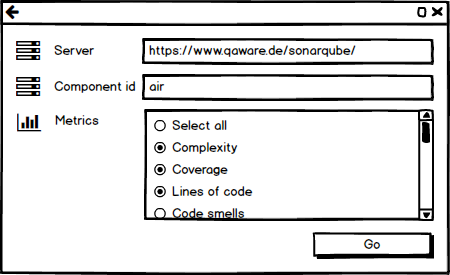
\includegraphics[width=.8\textwidth]{figures/sonarqube-import}
  \caption{Low-Fi Prototyp für den Import eines neuen Projekts anhand des Beispiels SonarQube}
  \label{fig:sonarqube-import}
\end{figure}

\begin{figure}[htb]
  \centering
  \begin{subfigure}[b]{\fwidth}
    \centering
    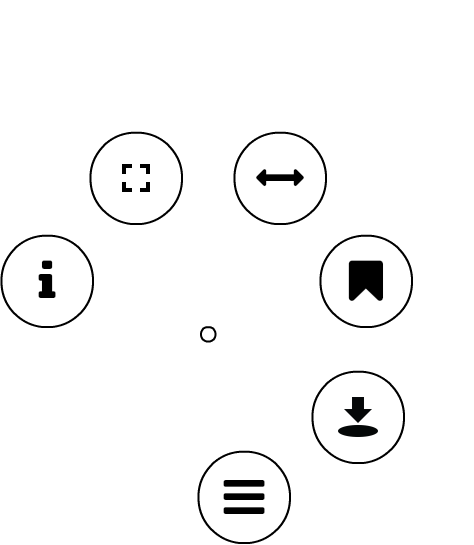
\includegraphics[scale=0.45]{figures/edge-contextmenu}
    \subcaption{Initialer Zustand} \label{fig:edge-contextmenu-initial}
  \end{subfigure}
  \hfill
  \begin{subfigure}[b]{\fwidth}
    \centering
    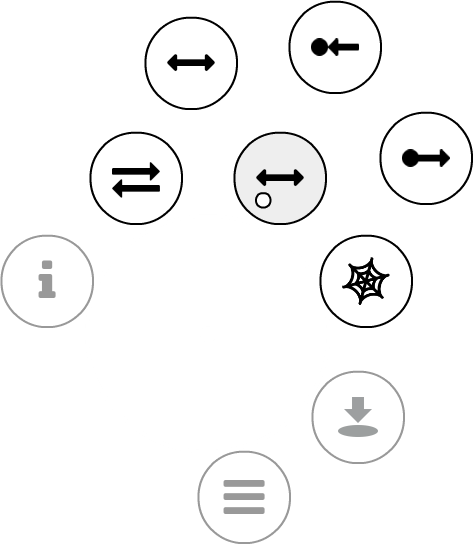
\includegraphics[scale=0.45]{figures/edge-contextmenu-connections}
    \subcaption{Unterauswahl für Verbindungen} \label{fig:edge-contextmenu-connections}
  \end{subfigure}
  \caption{Kontextmenü für einen inneren Knoten} \label{fig:edge-contextmenu}
\end{figure}

\begin{figure}[htb]
  \centering
  \begin{subfigure}[b]{\fwidth}
    \centering
    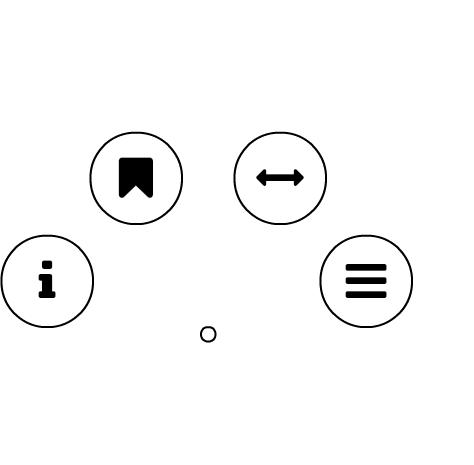
\includegraphics[scale=0.45]{figures/root-contextmenu}
    \subcaption{Initialer Zustand} \label{fig:root-contextmenu-initial}
  \end{subfigure}
  \hfill
  \begin{subfigure}[b]{\fwidth}
    \centering
    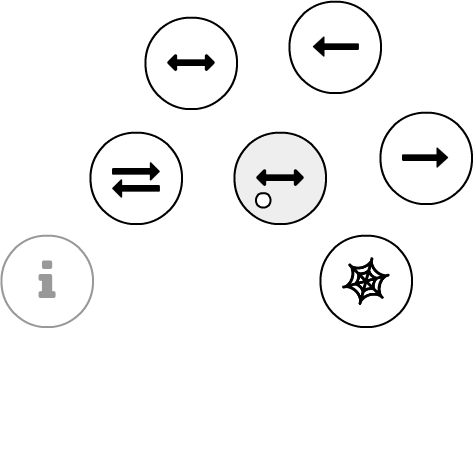
\includegraphics[scale=0.45]{figures/root-contextmenu-connections}
    \subcaption{Unterauswahl für Verbindungen} \label{fig:root-contextmenu-connections}
  \end{subfigure}
  \caption{Kontextmenü für eine Wurzel} \label{fig:root-contextmenu}
\end{figure}

\mainmatter

\pagestyle{scrheadings}
\addtokomafont{caption}{\small}
\chapter{Einleitung}

\begin{fquote}[Mark Zuckerberg][Facebook CEO][2014]
Virtual reality was once the dream of science fiction. But the internet was also once a dream, and so were computers and smartphones. The future is coming.
\end{fquote}

\begin{fquote}[Tim Cook][Apple CEO][2017]
I think AR is [...] big, it’s huge. I get excited because of the things that could be done that could improve a lot of lives.
\end{fquote}

\section{Einführung in die AR}
Viele der einflussreichsten Technologieunternehmen arbeiten an der \emph{Virtual} bzw.\ \emph{Augmented Reality (VR} bzw.\ \emph{AR)}. Tim Cook ist überzeugt davon, dass die AR die nächste \emph{``big idea''} nach dem Smartphone wird \cite{theindependent2017apple}.

Nicht nur Großkonzerne wie Apple, Facebook oder Samsung arbeiten intensiv in diesem Bereich. Ein Start-up-Unternehmen namens \emph{Magic Leap} entwickelt eine AR Brille und wird von Investoren in Billionenhöhe unterstützt \cite{kelly2016untold}. Laut einem Cover-Artikel der Zeitschrift \emph{Wire} ist die noch unter Verschluss gehaltene Technologie den Konkurrenzprodukten allen voraus. Das Release der Hardware ist Stand heute noch nicht bekannt, aber es lässt sich ein Trend erkennen, der die nächsten Jahre viele neue Möglichkeiten eröffnen wird und möglicherweise die Digitalisierung revolutionieren könnte.
Diese Arbeit wird sich mit einer Anwendung für die AR beschäftigen -- der Softwarevisualisierung. Die Spezialisierung auf AR kann nach der Abgrenzung von AR und VR besser nachvollzogen werden.

\paragraph{VR} ist eine Umgebung, in der der Betrachter vollkommen von einer computergenerierten Welt umgeben ist, die oft die reale Welt imitiert, aber auch rein fiktiv sein kann \cite{milgram1995augmented}.\\

Obwohl der Begriff AR zunehmend in der Industrie Verwendung findet, entbehrt er doch einer einheitlichen Definition. In \cite{azuma1997survey} wird AR als \emph{"`Variation"'} von VR betrachtet. Dagegen vermittelt Milgrim in \cite{milgram1995augmented} ein vollständigeres Verständnis, weshalb sich die Begrifflichkeiten in dieser Arbeit daran anlehnen sollen. Nach Milgrim existieren die beiden entgegengesetzten Extreme der Realität und der Virtualität. Alles dazwischen ist die sogenannte \emph{Mixed Reality (MR)}.

\paragraph{MR} ist eine Umgebung, in der Elemente der realen und einer virtuellen Welt zusammen dargestellt werden \cite{kato1999marker}.\\

\begin{figure}[htb]
  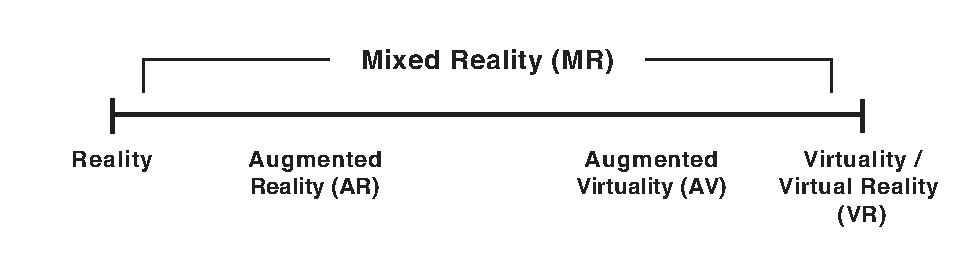
\includegraphics[width=.8\textwidth]{\figdir/rv-continuum}
  \caption{Abgewandelte Darstellung des Reality-Virtuality-Kontinuums aus \cite{milgram1995augmented}}
  \label{fig:rv-continuum}
\end{figure}

Dieses \emph{Reality-Virtuality-Kontinuum} ist in Abbildung \ref{fig:rv-continuum} dargestellt, in dem gut zu erkennen ist, dass AR zu der Mixed Reality gehört. In den meisten Quellen wie \cite{azuma1997survey, azuma2001recent, kato1999marker} wird bei der AR noch die Komponente der Interaktion aufgeführt. AR kann deshalb folgendermaßen definiert werden:

\begin{defbox}{AR}{ar}
   AR ist die Erweiterung der realen Welt durch computergenerierte Elemente, mit denen der Betrachter in Echtzeit interagieren kann.
\end{defbox}

Auch die \emph{Augmented Virtuality}, also die Erweiterung der virtuellen Welt durch reale Elemente, gehört zur MR.

Wie viele der einflussreichsten Menschen der Technologie-Industrie, sieht Tim Cook mehr Zukunft in der AR, da, wie er in einem Interview sagt, diese Technologie nicht wie die VR die wirkliche Welt ausschließt, sondern die Realität erweitert und Teil von zwischenmenschlicher Kommunikation sein kann \cite{theindependent2017apple}.

Wir stellen uns ein Hologramm vor, dass auf einem Konferenztisch Gestalt annimmt und ein Software-System repräsentiert. Entwickler, Projektleiter oder auch Kunden versammeln sich um den Tisch und können miteinander interaktiv die Software betrachten, evaluieren und wichtige Informationen daraus ziehen.

Dies wäre mit VR nicht möglich, da der Betrachter von der Außenwelt abgeschottet ist. Deshalb wird im Zuge dieser Arbeit mit der Stand heute am weitesten ausgereiften Technologie der AR gearbeitet -- der \emph{HoloLens} von Microsoft.

\section{Motivation dieser Arbeit}
Die Technologie der AR bietet uns viele neue Möglichkeiten. Eine Motivation dieser Arbeit ist es sich produktiv mit einer neuen, zukunftsträchtigen Technologie zu beschäftigen. Das ist jedoch nur die eine Seite. Die weitaus größere Motivation ist, die zuvor noch nicht dagewesene Zugänglichkeit und Interaktion mit dreidimensionaler \emph{Visualisierung} auszunutzen. Visualisierung im Allgemeinen begegnet uns in vielen Bereichen unseres Lebens und nimmt eine wichtige Rolle ein.

Niemand konnte bislang unser Sonnensystem von außen betrachten. Dennoch haben wir alle eine ziemlich gute Vorstellung wie dieses aufgebaut ist. Durch die Visualisierung der Planeten und der Sonne entsteht in uns ein geistiges Abbild der Realität. Das Konzept komplexe Realitäten zu abstrahieren und zu visualisieren, um dadurch die Realität besser verstehen zu können, ist in vielen Disziplinen der Wissenschaft vertreten.

Neben Wissenschaften wie Physik, Chemie oder Biologie, nimmt Visualisierung
auch besonders in der Informatik eine wichtige Rolle ein. In vielen Bereichen müssen Informationen in eine visuelle Form gebracht werden, die für das menschliche Auge besser zu lesen sind.

Gerade bei komplexen Software-Systemen ist das der Fall. Soll zum Beispiel die zu Grunde liegende Struktur einer Software Außenstehenden erklärt werden, gelingt das mit einem visuellen Modell wie einem UML-Diagramm sicherlich besser, als nur in den Source-Code zu schauen.

So wie UML-Diagramme, war die Darstellungsform der Softwarevisualisierung bislang meist zweidimensional. Mit AR wird dieser Disziplin der Visualisierung jedoch wortwörtlich ein neuer Raum an Möglichkeiten eröffnet und in diese Arbeit soll diesen Raum ausfüllen.

\section{Zielsetzung}
Für die Zielsetzung einer 3D Softwarevisualisierung in der AR sollten zunächst die allgemeinen Ziele einer Softwarevisualisierung betrachtet werden. Softwarevisualisierung ist für Diehl die "`visualization of artifacts related to software and its development process"' \cite{diehl2007software}. Wird der Fokus mehr auf die Ziele, d.h. den Nutzen für den Betrachter gelegt, lässt sich Softwarevisualisierung wie folgt definieren:

\begin{defbox}{Softwarevisualisierung}{software-visualization}
Softwarevisualisierung ist die bildliche oder auch metaphorische Darstellung einer Software, um dem Betrachter durch Vereinfachung und Abstraktion das bessere Verständnis oder die einfachere Analyse von Software zu ermöglichen.
\end{defbox}

In dieser Arbeit soll das neue Konzept \emph{CodeLeaves} für eine solche Softwarevisualisierung in der AR vorgestellt und im Detail ausgearbeitet werden.

Dabei soll CodeLeaves, im Vergleich zu andern 3D Softwarevisualisierungen, die Vorteile der Dreidimensionalität optimal ausnutzen.

Im Vorfeld dieser Arbeit wurden in einer Studie Metriken gesammelt, die eine gute Softwarevisualisierung bzw. CodeLeaves unterstützen sollte.

Es sollen dynamische und statische Metriken zur Erkennung von Anomalien in einer Software unterstützt werden. Ebenfalls soll die Darstellung der Struktur und der darauf abgebildeten Abhängigkeiten innerhalb einer Software möglich sein.

Durch weitere Expertengespräche sollen Userstories erstellt werden um den Mehrwert des neuen Konzepts validieren zu können.

Um diesen Anforderungen gerecht zu werden, soll für CodeLeaves ein sprachunabhängiges Datenmodell entworfen werden, dass alle geforderten Metriken unterstützt.

Der Praktische Teil dieser Arbeit soll die prototypische Entwicklung von CodeLeaves für die HoloLens sein.

\section{Aufbau der Arbeit}
Im Kapitel \ref{ch:concept} wird das Konzept von CodeLeaves vorgestellt. Dabei wird zunächst unter Betrachtung alternativer Ansätzen begründet, wieso ein neues Konzept sinnvoll ist, um dann in Abschnitt \ref{sec:idea} genauer auf das Konzept einzugehen. Die Befragung von Experten der Softwareanalyse und die daraus abgeleiteten Anforderungen an CodeLeaves in Abschnitt \ref{sec:requirements} schließen das erste Kapitel ab.

Das Kapitel \ref{ch:data-model} beschäftigt sich mit der Entwicklung eines geeigneten Datenmodells für CodeLeaves. Es werden vorhandene Datenmodelle auf Tauglichkeit für CodeLeaves überprüft und Rücksprache mit erfahrenen Software-Ingenieuren gehalten.

Aufbauend auf das entwickelte Datenmodell, wird das Konzept von CodeLeaves in Kapitel \ref{ch:layout} theoretisch weiter ausgearbeitet. Darunter fällt die Positionierung der Bäume auf einer Grundfläche und die Länge, Dicke und der Winkel der einzelnen Äste. Parallel zur Theorie wird aufgezeigt, wie sich CodeLeaves in Unity für die HoloLens modellieren lässt.

Die Interaktion mit CodeLeaves soll Thema des Kapitel \ref{ch:interaction-codeleaves} sein. Besonders die Abhängigkeiten von Artefakten einer Software sollen mithilfe von CodeLeaves interaktiv exploriert werden können.

Das Kapitel \ref{ch:conclusion} fasst die Ergebnisse der Arbeit zusammen und ein Ausblick auf zukünftige Verwendung und weiterführende Arbeiten runden die Arbeit ab.

\section{Abgrenzung}
\label{sec:distinction}

Die Beschaffung der Informationen über eine Software soll wird hier nur am Rande betrachtet. Für die Analyse einer Software müssen statische und dynamische Informationen gesammelt und aggregiert werden. Dafür gibt es verschiedenste Tools, wie inhouse Entwicklungen der QAware mit dem \textit{Software-EKG} und dem \textit{QAvalidator} oder proprietäre und Open-Source-Software. Die Anbindung an CodeLeaves würde den Rahmen dieser Arbeit jedoch sprengen.

Stattdessen soll der Fokus besonders auf das grundlegende Konzept und das Frontend mit der Generierung und Interaktion des Waldes gelegt werden. Diese Arbeit stellt jedoch den Anspruch, dass mit realistischen Daten gearbeitet wird, um eine valide Einschätzung des Mehrwerts von CodeLeaves geben zu können.

\chapter{Das Konzept CodeLeaves}
\label{ch:concept}

\section{CodeLeaves und die Metapher Software-Wald}
\label{sec:idea}

\emph{``Hierarchies are almost ubiquitous [...]''} \cite{robertson1991cone} halten Robertson \emph{et al.}
 schon 1991 bei der Visualisierung von hierarchischen Informationen fest. So auch bei der Struktur einer Software. Jede Software mit einer geschachtelten Paketstruktur ist hierarchisch und kann in einer Baumstruktur dargestellt werden. \emph{"`Bäume sind eine der wichtigsten Datenstrukturen, die besonders im Zusammenhang mit hierarchischen Abhängigkeiten und Beziehungen zwischen Daten von Vorteil sind."'} \cite{ernst2016grundkurs} stellen auch Ernst \emph{et al.} fest. Draus folgt, dass die Darstellung von Software als Baum oder auch Bäume sinnvoll ist.

Der Baum in der Informatik zeugt von einer ursprünglichen Metapher -- der Baum, wie er draußen in der Natur wächst. Da dieser unbestritten dreidimensional ist, liegt eine Softwarevisualisierung für die Dreidimensionalität mit einer realitätsnäheren Interpretation der Baum-Metapher nahe. Werden die Bäume, die im zweidimensionalen meist von oben nach unten gezeichnet wird, in 3D in natürlicher Wuchsrichtung modelliert und mehrere Bäume für eine Software verwendet, entsteht eine neue Metapher: der \emph{Software-Wald}.

CodeLeaves stellt ein Konzept dar, dass sich die Metapher des Software-Waldes zu nutze macht und wird im Folgenden auf High-Level-Ebene skizziert und danach genauer erläutert:

\begin{titlebox}{\textbf{Konzept:} CodeLeaves}
  \begin{enumerate}
    \item Die Struktur der Software wird mit nach oben wachsenden Bäumen dargestellt.
    \item Jedes Paket im \emph{Root-Verzeichnis} wird als einzelner Baum auf einer Ebene -- dem \emph{Waldboden} -- dargestellt.
    \item Die Blätter der Bäume entsprechen den Softwareartefakten (z.B. Klassen) und können durch ihre Farbe eine beliebigen Metrik visualisieren.
    \item Zwischen den Bäumen entsteht ein \emph{Wurzelgeflecht}, was die aggregierten Abhängigkeiten zwischen den Paketen darstellt.
    \item Abhängigkeiten oder Aufrufe zwischen einzelnen Softwareartefakten werden aggregiert über die Elternpakete als farbige bzw. Dicke der Äste dargestellt oder alternativ als direkte \emph{Spinnweben} zwischen den Bäumen.
  \end{enumerate}
\end{titlebox}

\paragraph{Punkt 1} ist dafür verantwortlich, dass die Softwarevisualisierung nahe an der tatsächlichen Software ist, wie sie ein Entwickler in seiner Code-Base gewöhnt ist. Das heißt, diejenigen, die auch tatsächlich mit der Software arbeiten, finden sich aufgrund der bekannten Baumstruktur auch in der Visualisierung schnell zurecht, ohne jedes Softwareartefakt auszuwählen, um zu sehen, mit welchem sie es zu tun haben. Im Fachjargon wird hier von der \emph{Habitability} gesprochen, also wie schnell oder gut sich ein Betrachter in einer Software oder auch deren Visualisierung "`zuhause"' fühlt \cite{wettel2007program}.

\paragraph{Punkt 2} ist weitgehend selbsterklärend. Durch Darstellung der Software in mehreren Bäumen entsteht erst der Software-Wald und die Pakete im Root-Verzeichnis als Wurzeln der Bäume zu verwenden bietet sich an. Das schließt jedoch nicht aus, dass Unterpakete als neuer Waldboden verwendet wird. Interaktion mit dem Waldboden soll Teil des Kapitel \ref{ch:interaction-codeleaves} sein.

\paragraph{Punkt 3} bedeutet, dass in CodeLeaves durch die Farbe der Blätter ein \emph{Laubdach} entsteht, dass eine gute Übersicht über eine ausgewählte Metrik der Software gibt. Beispielsweise kann der Farbe der Blätter die Code-Coverage der einzelnen Softwareartefakte (siehe Definition \ref{def:softartefact}) zugewiesen werden. Mit einer Skala von Grün bis Rot kann dann der Software-Wald bei guter Testabdeckung im sommerlichen Grün erstrahlen, oder bei einer weniger guten Coverage eher in den Herbst übergehen. Die Färbung des Laubdachs ist flexibel auf jegliche Metrik anwendbar, die bei der betrachteten Software zur Verfügung steht.

\begin{defbox}{Softwareartefakt}{softartefact}
  Ein Softwareartefakt wird in dieser Arbeit als Überbegriff für die kleinste betrachtete Einheit der Software verstanden. Das können bei objektorientieren Sprachen typischerweise Klassen, aber auch bei feinerer Granularität einzelne Funktionen innerhalb einer Klasse sein. Auch die Betrachtung von Dateien, die mehrere Klassen enthalten können, sind denkbar.
\end{defbox}

\paragraph{Punkt 4} bietet einen goßen Vorteil gegenüber der Zweidimensionalität. In Abbildung \ref{fig:3d-advantage} wird rechts das Prinzip des Wurzelgeflechts mit einem minimalistischen Beispiel illustriert.

\begin{figure}[htb]
  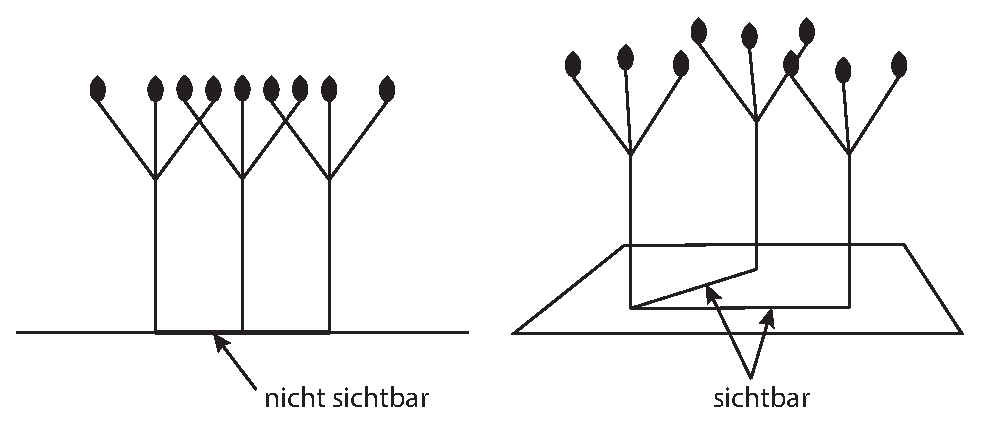
\includegraphics[width=.8\textwidth]{figures/3d-advantage}
  \caption{Vorteil der Dreidimensionalität bei der Darstellung von Abhängigkeiten}
  \label{fig:3d-advantage}
\end{figure}

Die Abhängigkeiten zwischen den Bäumen wird auf einen Blick ersichtlich. Betrachtet man die Bäume in 2D, wie es im linken Teil der Abbildung dargestellt ist, verschwinden die Abhängigkeiten hintereinander und sind nicht zuzuordnen.

\paragraph{Punkt 5} heißt, dass die Abhängigkeiten einer Software sehr übersichtlich auf die Struktur der Software abgebildet werden können, ohne diese zu beeinflussen. Für das besser Verständnis bedarf es einer Definition der Aggregation von Abhängigkeiteän.

\begin{splitbox}{Aggregation von Abhängigkeiten}{aggregation}
Bei der Aggregation von Abhängigkeiten zwischen Softwareartefakten werden die Abhängigkeiten nicht direkt dargestellt, sondern über die Eltern-Pakete geleitet. Seien $x, y$ Pakete und Softwareartefakt $A \in x$ besitze eine Abhängigkeit zu Softwareartefakt $B \in y$, dann geht die Abhängigkeit von $A$ zu einem zusätzlich Konstrukt $\Psi_x$, das das Pakets $x$ repräsentiert. Angenommen $x$ und $y$ befinden sich zudem im Paket $z$, dann geht die aggregierte Abhängigkeit entweder direkt von $\Psi_x$ zu $\Psi_y$, oder weiter über $\Psi_z$ zu $\Psi_y$ und schließlich $B$.
\tcblower
%\raggedright
%Beispiel in CodeLeaves:\par\vspace{.6cm}
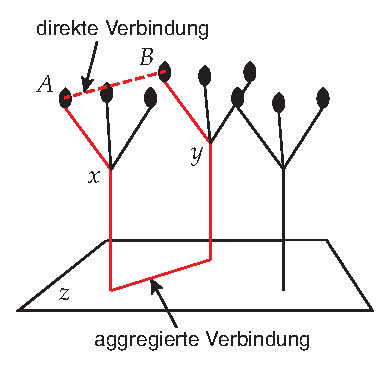
\includegraphics[width=\linewidth]{figures/aggregation}
\end{splitbox}

Auf der rechten Seite der Definition \ref{def:aggregation} ist eine aggregierte Abhängigkeit am Beispiel von CodeLeaves zu sehen. Die $\Psi$ in CodeLeaves sind die Knoten der Bäume, an denen die Äste zusammen laufen und im Spezialfall des Root-Verzeichnisses, der Waldboden.

Bei mehreren Abhängigkeiten zwischen Nachbar-Paketen, überlagern sich die aggregierten Abhängigkeiten zwangsläufig. Falls in unserem Beispiel eine weitere Abhängigkeit von Paket $x$ zu Paket $y$ bestünde, würden sich die Abhängigkeiten von $\Psi_x$ bis $\Psi_y$ überlagern. Daraus ergibt sich, dass nicht jede aggregierte Abhängigkeit ohne Interaktion zwangsläufig eindeutig zuzuordnen ist.

Wird aber bei jeder Kante, sei es ein Ast, Stamm, oder Wurzel, die Anzahl an überlagernden Abhängigkeiten als Dicke der Kante dargestellt, bekommt der Betrachter eine gute Übersicht über die Gesamtheit der Abhängigkeiten. Durch Interaktion mit einzelnen Kanten, oder sogar des ganzen Waldbodens, soll eine fein granulärere Analyse der Abhängigkeiten möglich sein.

Das zweite Element von Punkt 5 sind die Spinnweben. Damit lassen sich die Abhängigkeiten direkt darstellen. Um bei großen Software-Systemen aber die Übersicht über den Wald nicht zu verlieren, sollten diese mithilfe der Interaktion des Nutzers flexibel aktivierbar sein.

Nachdem das grundlegende Konzept von CodeLeaves verstanden ist, muss eine Begriffsdefinition ein Einheitliches Verständnis der verwendeten Komponenten schaffen. Die eingeführten Bezeichnungen dienen dem Verständnis der verwendeten Datenmodelle im nächsten Kapitel, sowie die entwickelten Layout-Algorithmen in Kapitel \ref{ch:layout}.

Die Struktur von CodeLeaves baut stark auf der Datenstruktur eines klassischen Baumes auf -- \textit{"`the most important nonlinear structures that arise in computer algorithms"'}\cite{knuth1973fundamental} -- die zum Beispiel in \cite{knuth1973fundamental, ernst2016grundkurs, gumm2009einfuehrung} definiert wird.

Da aber die Struktur von CodeLeaves zum Teil von der klassischen Definition abweicht und teilweise neue Bezeichnungen benötigt, betrachten wir daher einige Definitionen zur Baumstruktur, um diese an die Gegebenheiten von CodeLeaves anzupassen und führen neue Begriffe ein.

\section{Begriffsklärung}
\label{sec:naming}

\begin{itemize}
  \item Ein \textit{Baum} (engl.: \textit{tree}) besteht aus einer Menge von \textit{Knoten}, die so durch \textit{Kanten} verbunden sind, dass keine Kreise auftreten (Abgewandelt aus \cite{gumm2009einfuehrung, ernst2016grundkurs}).
  \item Ein \textit{Knoten} beinhaltet Informationen zu sich selbst und hat $0$ bis $n$ \textit{Kinder} (auch Nachfahren genannt, engl.: \textit{childs} oder \textit{descendant}).
  \item Ein Knoten mit keinen Kindern wird als \textit{Blatt} (engl.: \textit{leaf}) bezeichnet. Alle anderen Knoten heißen \textit{innere Knoten} (engl.: \textit{innerNode}) \cite{gumm2009einfuehrung}.
  \item Kinder des selben Knotens werden \textit{Geschwister} (engl.: \textit{siblings}) genannt.
\end{itemize}

Bei der klassischen Definition eines Baumes wird bei dem Knoten ohne Elternteil von der "`Wurzel"' gesprochen. Im Modell von CodeLeaves ist der unterste Knoten des Baumes jedoch noch durch eine Kante mit dem Waldboden verbunden. Darüber hinaus überschneidet sich die Bezeichnung von "`Wurzel"' mit den Verbindungen zwischen den einzelnen Bäumen, die bei der klassischen Definition nicht existieren. Deshalb wird für diesen speziellen Knoten eine neue Bezeichnung eingeführt.

\begin{itemize}
  \item Der unterste Knoten eines Baumes wird als \textit{Kronenansatz} (engl.: \textit{crown base}) bezeichnet.
  \item Alle Knoten bis auf den Kronenansatz haben genau einen Knoten als \textit{Elternteil} (auch Vorfahre genannt, engl.: \textit{parent} oder \textit{ancestor}).
\end{itemize}

Nachdem in den meisten Fällen Bäume in 2D nach unten wachsend dargestellt werden, was wahrscheinlich auf die Tatsache zurück zu führen ist, dass handschriftliche Diagramme tendenziell nach unten wachsend gezeichnet werden \cite{knuth1973fundamental}, wird bei Knoten auch oft von einer Tiefe gesprochen. Diese Bezeichnung wird beibehalten.

\begin{itemize}
  \item Die \textit{Tiefe} eines Knotens gibt an, wie viele Kanten er vom Kronenansatz aus entfernt liegt (Abgewandelt aus \cite{ernst2016grundkurs}).
  \item Die \textit{Höhe} (engl.: \textit{height}) eines Knoten beschreibt die maximale Tiefe aller Nachfahren.
  \item Alle Knoten mit der gleichen Höhe befinden sich auf der selben \textit{Ebene}
\end{itemize}

Alle nachfolgenden Kanten und Knoten eines Knotens $A$ werden in der Literatur unterschiedlich bezeichnet. Es ist die Rede von "`Teilbaum"' \cite{ernst2016grundkurs} oder auch "`Unterbäumen"' \cite{gumm2009einfuehrung}. Wir definieren dafür einen dem 3D Modell besser entsprechenden Begriff.

\begin{itemize}
  \item Ein \textit{Ast} (engl.: \textit{branch}) sind alle nachfolgenden Kanten und Knoten des Knotens $A$ ausschließlich des Knotens $A$ selbst.
\end{itemize}

Bisher wurden Bezeichnungen aus einschlägiger Literatur verwendet oder abgeändert. Betrachten wir nun Elemente von CodeLeaves, die so nicht in der klassischen Definition einer Baumes vorkommen.

\begin{itemize}
  \item Der Kronenansatz ist durch die Kante namens \textit{Stamm} (engl.: \textit{trunk}) mit den \textit{Waldboden} (engl.: forest floor) verbunden.
  \item Der Schnittpunkt zwischen Stamm und Waldboden nennen wir \textit{Stammbasis} (engl.: \textit{trunk base}). Dieser ist jedoch kein Knoten und beinhaltet auch keine Informationen.
  \item Ein \textit{Wald} besteht aus einer disjunkten Menge an Bäumen und dem Waldboden.
  \item Ein Waldboden eines Waldes mit $n$ Bäumen besitzt $0$ bis $n!$ \textit{Wurzeln} (engl. \textit{roots}), die jeweils zwei Stammbasen miteinander verbinden.
\end{itemize}

\begin{figure}[htb]
  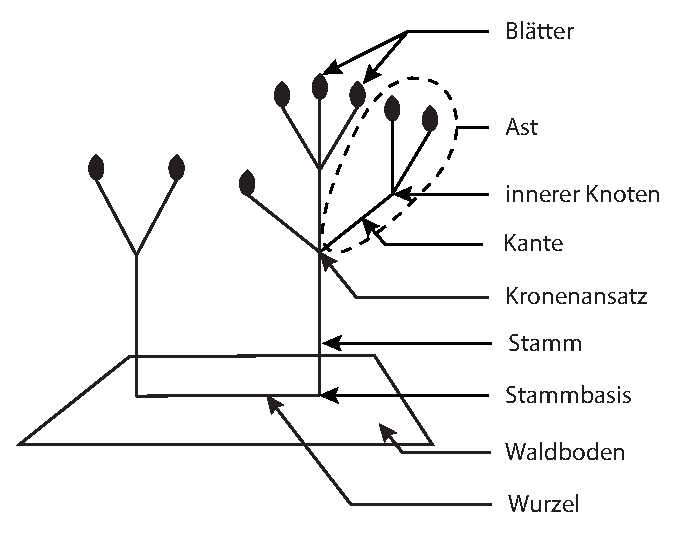
\includegraphics[width=.6\textwidth]{\figdir/naming}
  \caption{Bezeichnungen}
  \label{fig:naming}
\end{figure}

\section{Vergleich mit anderen Konzepten}
\label{sec:comparison}

Im Vorfeld dieser Arbeit wurde in \cite{puetz2017softwarevisualisierung} evaluiert, was eine gute Softwarevisualisierung ausmacht und unterstützen sollte. Ausgehend davon, wurden vorhandene 3D Visualisierungen und andere mögliche Konzepte miteinander verglichen. Die Ergebnisse dieser Untersuchung, soll in Folgenden vorgestellt werden.

Um herauszufinden welchen Mehrwert sich Nutzer einer Softwarevisualisierung von dieser versprechen, wurde eine Umfrage in der QAware GbmH durchgeführt. Die QAware ist ein Projekthaus mit den Kerngeschäften Diagnose, Sanierung, Exploration und Realisierung von Software \cite{qaware2017it-probleme}. Durch die Erfahrung in Projekten für namhafte Kunden, zeichnen sich die Mitarbeiter durch fundiertes Wissen und Expertise aus. Es wurden insgesamt 22 Mitarbeiter mit unterschiedlichen Rollen in der Softwareentwicklung befragt.

\begin{figure}[hbt]
\begin{tikzpicture}
  \begin{axis} [
    width = \textwidth,
    height = 8cm,
    symbolic x coords={Lines of Code, Komplexität, Coverage, Struktur, Abhängigkeiten, Code-Violations, Anzahl Aufrufe, Ausführungszeiten, Laufzeitfehler, Ressourcen-Auslastung, Evolution der Statik, Evolution eins Themas},
    xtick={Lines of Code, Komplexität, Coverage, Struktur, Abhängigkeiten, Code-Violations, Anzahl Aufrufe, Ausführungszeiten, Laufzeitfehler, Ressourcen-Auslastung, Evolution der Statik, Evolution eins Themas},
    x tick label style={rotate=45, anchor=east, align=center},
    major x tick style = transparent,
    axis lines = left,
    axis line style = {-},
    ymajorgrids = true,
    ylabel=Anzahl,
    legend style = {at={(.99,.98)}, anchor=north east, legend columns=-1, column sep=1ex},
    ymin=0,
    bar width=5mm,
    ybar=-0.5cm,
    enlarge x limits={abs=0.6cm}
  ]
    \addplot[style={fill=primary}]
      coordinates {(Lines of Code, 1) (Komplexität, 3) (Coverage, 1) (Struktur, 5) (Abhängigkeiten, 7) (Code-Violations, 4)};
    \addplot[style={fill=secondary}]
      coordinates {(Anzahl Aufrufe, 5) (Ausführungszeiten, 5) (Laufzeitfehler, 1) (Ressourcen-Auslastung, 1)};
    \addplot[style={fill=tertiary}]
      coordinates {(Evolution der Statik, 3) (Evolution eins Themas, 1)};

    \legend{Statik, Dynamik, Evolution}

  \end{axis}
\end{tikzpicture}
\caption{Von Mitarbeitern der QAware gewünschte Informationen} \label{fig:survey}
\end{figure}

In Abbildung \ref{fig:survey} ist zu sehen, wie oft welche Metriken genannt wurden. Alle Metriken lassen sich in die drei Kategorien der Softwarevisualisierung aus \cite{diehl2007software} einordnen und sind farbig entsprechend gruppiert.

\paragraph{Statik} sind die Informationen, die ohne die Ausführung der Software generiert werden können \cite{diehl2007software}. Darunter fallen die Metriken, die als Zahl zu jedem Softwareartefakt zugeordnet werden können und damit zueinander in Relation gesetzt werden können. Genannt wurden LOC, Komplexität, Coverage und Code-Violations. Letzteres sind beispielsweise Verletzungen von vereinbarten \emph{Code-Conventions}. Die Informationen, die komplizierter zu visualisieren sind, stellen die Struktur und die Abhängigkeiten dar. Aus Abbildung \ref{fig:survey} geht hervor, dass diese Informationen gleichzeitig am meisten von Interesse sind.

\paragraph{Dynamik} beschreibt die Informationen, die zur Laufzeit einer Software generiert werden können \cite{diehl2007software}. Besonders oft wurden Ausführungszeiten von Softwareartefakten und Anzahl von Aufrufen genannt. Damit sind beispielsweise \emph{Bottlenecks} identifizierbar. Auch die Darstellung der Laufzeitfehler einer fehlerhaften Software sind für deren Analyse wichtig. Die Resourcen-Auslastung ist dabei auch hilfreich, wirkt sich jedoch wenig auf das 3D Modell der Softwarevisualisierung aus, da diese Informationen parallel zur eigentlichen Software existieren.

\paragraph{Evolution} beschreibt den zeitlichen Verlauf einer Software und stellt den Entwicklungsprozess in den Vordergrund \cite{diehl2007software}. Beispielsweise kann die Entwicklung statischer Metriken verfolgt werden. Mit der Evolution eines Themas ist gemeint, dass anhand die Entwicklung eines bestimmten Themas nachverfolgt werden kann.\\

Aus den von den Mitarbeiten gewünschten Informationen und weitern Rahmenbedingungen wurde in \cite{puetz2017softwarevisualisierung} folgende Kriterien aufgestellt, anhand derer vier verschiedene Modelle der 3D Softwarevisualisierung bewertet wurden.

\begin{itemize}
  \item Statische Metriken (z.B. Komplexität)
  \item Struktur
  \item Abhängigkeiten
  \item Dynamik (Primär Ausführungszeiten und Anzahl der Aufrufe)
  \item Evolution
  \item Habitability (vgl. Kapitel \ref{ch:concept} Punkt 1)
  \item Drilldown
  \item Technische Machbarkeit
\end{itemize}

Bei dem Kriterium Drilldown wurde bewertet, wie gut eine Visualisierung ihre Informationen von High-Level, bis hin zu Details darstellen kann.

Bei der technischen Machbarkeit wurde berücksichtigt, ob eine existierende Softwarevisualisierung für die HoloLens verwendbar ist. In Abbildung \ref{fig:alternatives} sind die untersuchten Alternativen abgebildet, darunter auch ein erster Entwurf von CodeLeaves.

\subsubsection*{CodeCity}
2007 stellten Wettel et al. CodeCity vor, die mithilfe der \textit{Stadt-Metapher} dreidimensionale Städte visualisiert, in denen Klassen als Gebäude und Pakete als Stadtviertel dargestellt werden \cite{wettel2007program, wettel2008visual, wettel2011software}. Für die Breite und Tiefe der Gebäude wurde für die Anzahl der Attribute (engl. \emph{number of attributes (NOA)}) und für die Höhe die Anzahl der Methoden (engl. \emph{number of methods (NOM)}) der visualisierten Klasse gewählt.

Die CodeCity ist als Konzept sehr durchdacht, bietet durch die Metapher gute Habitability und unterstützt die Darstellung der Evolution. Auch soll nach Wettel et al. die CodeCity die Analyse von Software im Vergleich zu herkömmlichen Analyse-Werkzeugen signifikant verbessern \cite{wettel2011software}.

Jedoch unterstützt CodeCity keine Dynamik und die Abhängigkeiten sind nur als direkte Verbindungen darstellbar, was bei größeren Software-Systemen sehr unübersichtlich wird. Die verfügbaren statischen Metriken sind begrenzt und vor allem ist die Technologie Stand heute nicht mehr produktiv einsetzbar \cite{puetz2017softwarevisualisierung}.

\newlength\fwidth
\setlength{\fwidth}{.49\textwidth}
\begin{figure}[htb]
  \centering
  \begin{subfigure}[b]{\fwidth}
   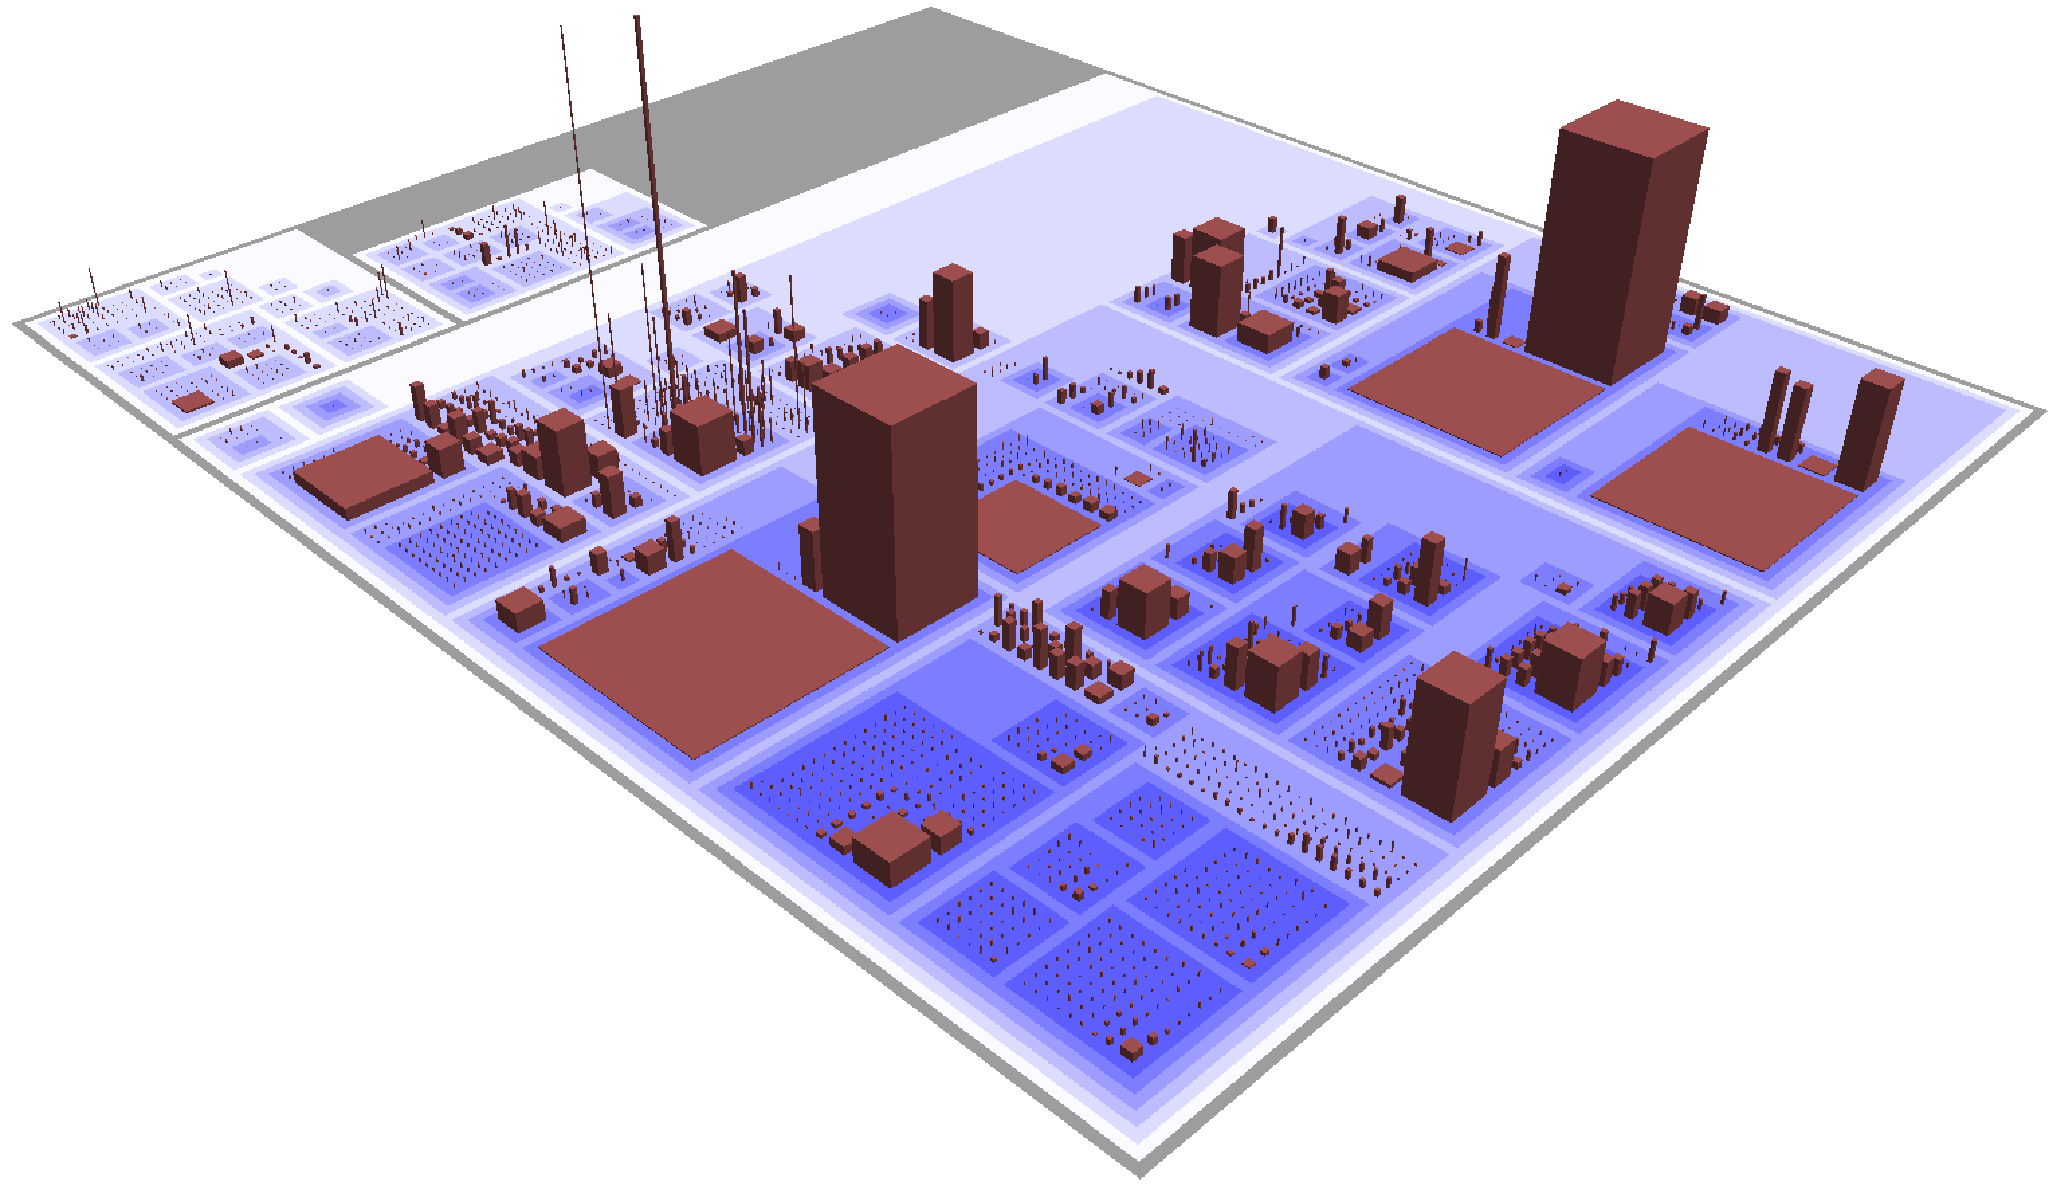
\includegraphics[width=\textwidth]{figures/code-city}
   \subcaption{CodeCity von ArgoUML \cite{wettel2008visual}} \label{fig:code-city}
  \end{subfigure}
  \hfill
  \begin{subfigure}[b]{\fwidth}
  	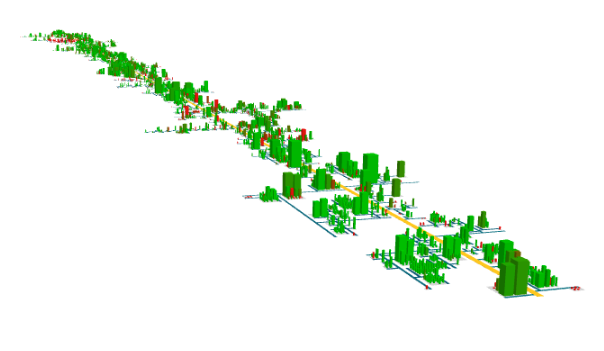
\includegraphics[width=\textwidth]{figures/softvis3d}
  	\subcaption{SoftVis3D mit Evostreet Layout} \label{fig:softvis3d}
  \end{subfigure}
  \hfill
  \vspace{1em}
  \begin{subfigure}[b]{\fwidth}
  	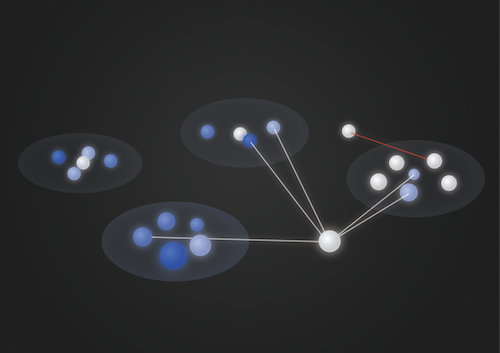
\includegraphics[width=\textwidth]{figures/code-universe}
  	\subcaption{Entwurf eines CodeUniverse} \label{fig:code-universe}
  \end{subfigure}
  \hfill
  \begin{subfigure}[b]{\fwidth}
  	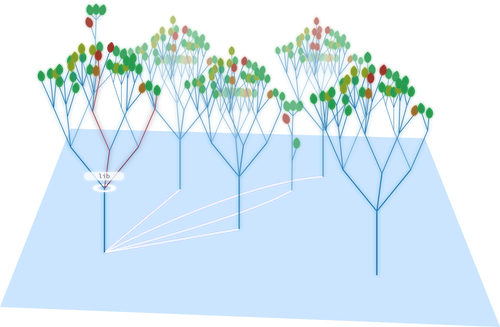
\includegraphics[width=\textwidth]{figures/code-leaves}
  	\subcaption{Erster Entwurf von CodeLeaves} \label{fig:code-leaves}
  \end{subfigure}
  \caption{CodeLeaves und alternative Modelle} \label{fig:alternatives}
\end{figure}

\subsubsection*{SoftVis3D}
SoftVis3D greift das Konzept der CodeCity auf und visualisiert als Plugin für SonarQube\footnote{SonarQube ist eine open-source Plattform für statische Code-Qualität, \url{https://www.sonarqube.org/}} Projekte direkt im Browser. Durch die direkte Anbindung an SonarQube, ist SoftVis3D hoch konfigurierbar und kann alle Metriken darstellen, die auch in SonarQube zur Verfügung. Neben dem \emph{District-Layout}, wie es in der CodeCity verwendet wird, unterstützt SoftVis3D darüber hinaus auch des \emph{Evostreet-Layout}, das ursprünglich in \cite{steinbruckner2013consistent} für die Evolution einer Software entworfen wurde. In diesem Layout, wie es in Abbildung \ref{fig:softvis3d} zu sehen ist, werden Pakete als Straßen dargestellt.

Die Evolution wird von SoftVis3D trotz Evostreet-Layout jedoch nicht unterstützt. Bei Die Abhängigkeiten wurde in früheren Versionen aggregiert dargestellt. Dafür wurden Pakete im Distrikt-Layout in übereinander liegenden Ebenen abgebildet und für $\Psi$ (vgl. Definition \ref{def:aggregation}) ein Hilfsgebäude benutzt, dass zu der darüberliegenden Ebene führt. Dadurch ging jedoch die Stadt-Metapher und die Übersichtlichkeit verloren. Die Dynamik kann in SoftVis3D ebenfalls nicht visualisiert werden. Die verwendete Technologie ist zwar mit \emph{WebGL} für den Browser State of the Art, aber für die HoloLens aktuell noch nicht sinnvoll einsetzbar \cite{puetz2017softwarevisualisierung}.

\subsubsection*{CodeUniverse}

Im Zuge der der Studie \cite{puetz2017softwarevisualisierung} wurde eine weitere Metapher evaluiert. Ähnlich wie in der Arbeit \cite{graham2004solar, balzer2004software}, wird die Software als Universum dargestellt. Die Softwareartefakte in Paketen gruppieren sich als Sterne in Galaxien. Statische Metriken können dann als Farbe und Größe der Sterne widergespiegelt werden. So können "`weiße Zwerge"' bis hin zu "`roten Riesen"' entstehen.

Das CodeUniverse ist für statische Metriken gut geeignet. Auch die Evolution ist mit der Entstehung von neuen Sternen und Galaxien gut vorstellbar. Die Struktur der Software ist zwar mit der Gruppierung der Sterne gegeben, aber weniger offensichtlich wie andere Konzepte. Bei der Visualisierung der Abhängigkeiten stößt das CodeUniverse aber an seine Grenzen. Durch direkte Verbindungen zwischen den Sternen lassen sich zwar Abhängigkeiten darstellen, aber bei großen Software-Systemen würde das schnell im Chaos enden. Auch in \cite{balzer2004software} wird beschrieben, dass eine übersichtliche Darstellung von Abhängigkeiten nur durch deren Aggregation erreicht werden kann. Deshalb wird in \cite{balzer2004software} ein Konzept entworfen, dass die Softwareartefakte mit einem \emph{"`hierarchischem Netz"'} verbindet. Dieses ist nichts anderes als die vorhandene Baumstruktur der Software und hat mit der Metapher des Universums auch nichts mehr zu tun. Folglich wären wir wieder bei dem neuen Konzept CodeLeaves angelangt.


\subsubsection*{Vorteile von CodeLeaves gegenüber anderen 3D Softwarevisualisierungen}
Die betrachteten Alternativen und weitere, haben gemein, dass sie zum einen Struktur, Dynamik und Evolution nicht vereinen. Zum anderen können Abhängigkeiten oder dynamische Aufrufe zwischen Softwareartefakten nicht ohne Verlust der Übersichtlichkeit angezeigt werden. CodeLeaves soll alle drei Kategorien der Softwarevisualisierung unterstützen und ist bei der Visualisierung der Struktur und der Abhängigkeiten den Alternativen überlegen. Durch die Baumstruktur, wie er auch in der Code-Base vorhanden ist, wird die Paket-Struktur eins zu eins wiedergegeben. Die aggregierten Abhängigkeiten lehnen sich an die Struktur an und beeinflussen diese nicht negativ. Durch das Wurzelgeflecht und die Spinnweben wird die Dreidimensionalität optimal ausgenutzt.

\section{Anforderungen an CodeLeaves}
\label{sec:requirements}

Die Umfrage, die in Abschnitt \ref{sec:comparison} vorgestellt wurde, ergab einen gutes Stimmungsbarometer über die Wünsche im Bezug auf zu visualisierend Informationen. In diesem Abschnitt soll genauer auf die Anforderungen an einen Software-Wald eingegangen werden. Dazu wurden von der QAware zwei Experten der Softwareanalyse zu diesem Thema befragt, um Userstories für CodeLeaves zu sammeln.

Aus der dynamischen Analyse wurde der promovierende Performance-Analyst F. Lautenschlager befragt. Dieser erarbeitete im Zuge seiner Dissertation eine hochperformante Zeitreihendatenbank zur Speicherung und Auswertung von dynamischen Daten einer Software und ist Experte auf diesem Gebiet.

Als Experte der statischen Analyse wurde J. Weigend befragt. Dieser ist Chefarchitekt, Geschäftsführer und Mitgründer der QAware. Er studierte Informatik mit Schwerpunkt "Verteilte Systeme" an der Hochschule Rosenheim und hält dort seit 2001 Vorlesungen \cite{qaware2017johannes}.

Im Folgenden werden die Gespräche mit den beiden Experten unter Anwendung der Methoden aus \cite{cohn2004user} in Userstories und in den Tabellen \ref{tab:acceptance1} -- \ref{tab:acceptance5} zu den dazugehörige Akzeptanzkriterien zusammengefasst. Zum Großteil überschneiden sich die Userstories mit der Umfrage aus Abschnitt \ref{sec:comparison}, was für eine gute Übereinstimmung der eingeholten Informationen spricht.

\begin{userstory}{Dynamische Metriken}
  Als \textit{Performance-Analyst}\\
  möchte ich \textit{Funktionsaufrufe, deren Antwortzeiten, Laufzeitfehler und Resourcen-Auslastung visualisiert haben},\\
  um \textit{das Laufzeitverhalten der Software in einem bestimmten Zeitraum explorativ bewerten zu können.}
\end{userstory}

\newcommand{\tableheader}{
\endfirsthead
\multicolumn{2}{l}{\small \tablename\ \thetable\ -- \textit{Fortsetzung von vorheriger Seite}} \\
\hline
  \endhead
  \hline
  \endlastfoot
  \hline
\multicolumn{2}{r}{\textit{\small Fortsetzung auf nächster Seite...}} \\
\endfoot
\hline
}
\renewcommand{\arraystretch}{1.5}
\begin{tabularx}{\textwidth}{lX}
	\caption{Akzeptanzkriterien zu Userstory 1}\label{tab:acceptance1} \\
	\tableheader
    1 & Antwortzeiten und Laufzeitfehler können als Metrik auf die Farbe der Blätter angewandt werden.\\
    2 & Wenn ich ein Blatt auswähle, dann kann ich die genaue Zahl der gerade betrachteten Metrik sehen.\\
    3 & Wenn ich ein Blatt auswähle, kann ich sehen wohin von dieser Klasse Aufrufe hin- bzw. eingehen.\\
    4 & Die Dicke einer Verbindung (d.h. ein Stück Ast oder Wurzel) zeigt mir die Anzahl der Aufrufe zwischen Anfang und Ende der Verbindung.\\
    5 & Wenn ich eine Verbindung anklicke, dann kann ich sehen, welche Klassen von dieser Verbindung betroffen sind.\\
    6 & Wenn ich eine Verbindung anklicke, dann kann ich sehen in welche Richtung die meisten betroffenen Verbindungen gehen.\\
    7 & Wenn ich den Wald als ganzes auswähle, dann kann ich den Zeitraum auswählen, auf die sich die dargestellten Daten beziehen.
\end{tabularx}

\begin{userstory}{Zustand der Software}
  Als \textit{Systemverantwortlicher}\\
  möchte ich \textit{auf einen Blick den Zustand meiner Software erkennen},\\
  um \textit{bei Bedarf agieren zu können}.
\end{userstory}

\begin{tabularx}{\textwidth}{lX}
	\caption{Akzeptanzkriterien zu Userstory 2} \\
	\tableheader
    1 & Wenn ich die Laubfarbe des Waldes betrachte, dann möchte ich eine möglichst gute Gesamtübersicht über die ausgewählte Metrik haben.\\
    2 & Wenn ich die Laubfarbe des Waldes betrachte, dann kann ich Ausreißer der ausgewählten Metrik gut erkennen.\\
    3 & Die Struktur der Bäume ist möglichst übersichtlich und hat keine Überlappungen.
\end{tabularx}

\begin{userstory}{Kopplung und Struktur}
  Als \textit{Softwarearchiteckt}\\
  möchte ich \textit{die Kopplung und Struktur einer großen Software sehen},\\
  um \textit{die Zusammenhänge zu verstehen}.
\end{userstory}

\begin{tabularx}{\textwidth}{lX}
	\caption{Akzeptanzkriterien zu Userstory 3} \\
	\tableheader
    1 & Die Paketstruktur entspricht der Struktur der Bäume.\\
    2 & Wenn ich die Verbindungen zwischen einzelnen Bäumen oder Verzweigungen betrachte, dann erkenne ich durch die Dicke, wie stark die Pakete aneinander gekoppelt sind.\\
    3 & Wenn ich ein Blatt auswähle, dann kann ich die ein- bzw. ausgehenden Abhängigkeiten hervorheben.\\
    4 & Wenn ich ein Blatt auswähle, dann kann ich Abhängigkeiten direkt als Spinnweben darstellen.\\
    5 & Wenn ich eine Verbindung auswähle, dann kann ich die von den Abhängigkeiten betroffenen Klassen hervorheben.\\
    6 & Wenn ich eine Verbindung auswähle, dann kann ich sehen wie viele Abhängigkeiten in welche Richtung fließen.\\
    7 & Wenn ich auswähle, dass zyklische Abhängigkeiten hervorgehoben werden, können diese direkt als Spinnweben im gesamten Wald dargestellt werden.
\end{tabularx}

\begin{userstory}{Code-Qualität}
  Als \textit{Softwarearchitekt}\\
  möchte ich \textit{Code-Qualität auf die Struktur abbilden können},\\
  um \textit{Anomalien und Qualitätsdefizite zu erkennen}.
\end{userstory}

\begin{tabularx}{\textwidth}{lX}
	\caption{Akzeptanzkriterien zu Userstory 4} \\
	\tableheader
    1 & Statische Metriken der Code-Qualität, wie z.B. Code-Coverage, kann auf die Farbe der Blätter angewandt werden.\\
    2 & Wenn ich die Laubfarbe des Waldes betrachte, dann kann ich Ausreißer der ausgewählten Metrik gut erkennen.
\end{tabularx}

\begin{userstory}{Code-Qualität}
  Als \textit{Softwarearchitekt}\\
  möchte ich \textit{einen intuitiven Drilldown haben},\\
  um \textit{die Zusammenhänge auf verschiedener Pakte-Ebene zu verstehen}.
\end{userstory}

\begin{tabularx}{\textwidth}{lX}
	\caption{Akzeptanzkriterien zu Userstory 5}\label{tab:acceptance5} \\
	\tableheader
    1 & Wenn ich eine Verbindung auswähle, dann kann ich das repräsentierte Paket als neuen Waldboden festlegen. \\
    2 & Wenn ich die Laubfarbe des Waldes betrachte, dann kann ich Ausreißer der ausgewählten Metrik gut erkennen.
\end{tabularx}

Bei der Entwicklung der Datenmodelle im nächsten Kapitel fließen die Userstories und Akzeptanzkriterien mit ein.

\chapter{Datenmodell}
\label{ch:data-model}
\section{Trennung in Schichten}
\label{ch:data-layers}

Das Datenmodell für CodeLeaves nimmt einen zentralen Baustein ein, auf den sich die Implementierung stützt. Bei dem Entwurfsmuster sind einige Prinzipien zu beachten. Wie Buschmann et al. in \cite{frank2007pattern} beschreibt, ist das Pattern \textit{Layers} ein Grundprinzip bei Software-Architekturen. Durch die \textit{Separation of concerns} werden einzelnen Schichten voneinander getrennt und können so später leichter ausgetauscht werden:

``Using semi-independent parts [...] enables the easier exchange of individual parts at a later date.`` \cite{frank2007pattern}

\subsubsection*{Backend}
Gerade bei der Visualisierung von abstrakten Daten, wie es eine Software ist, ist eine Schichtentrennung besonders wichtig. CodeLeaves hat das Ziel eine beliebige objektorientierte Software darstellen zu können. Da aber nicht für jede Programmiersprache CodeLeaves angepasst werden soll und die Informationen über die Software aus unterschiedlichen Quellen stammen können, ist hier die erste Schicht \textit{Backend} sinnvoll. Im Backend Layer werden die Daten über eine Software aggregiert, seien es statische oder dynamische Informationen und in ein Sprach-agnostisches Format gebracht. Die Konnektoren, d.h. die Verbindungen zu den verschiedenen Datenquellen, können dann leicht ausgetauscht werden.

Wie in Abschnitt \ref{sec:distinction} bereits festgehalten, soll der Schritt des Transfers der realen Software in deren Repräsentation jedoch nicht Schwerpunkt dieser Arbeit sein. Das Datenmodell ist hingegen sehr wohl zu definieren, um die Daten darstellen zu können.

\subsubsection*{Application logic}
Die Einteilung in Schichten geht nach der Transformation der Software in ein Meta-Modell aber noch weiter. CodeLeaves könnte neben Software prinzipiell auch jegliche anderen, hierarchisch strukturierten Informationen darstellen. Für die interne Datenhaltung wird deshalb in der Schicht \textit{Application logic} das Datenmodell weiter abstrahiert und in ein Format gebracht, dass sich stark an der Baumstruktur der Informatik orientiert. So könnten später auch leicht gänzlich andere Daten angebunden werden.

\subsubsection*{Presentation}
Die letzte Schicht ist die der \textit{Presentation}. Das Datenmodell für hierarchische Informationen muss für die Darstellung der Bäume weiter verarbeitet werden. Zum Beispiel muss für die rekursive Generierung der Bäume die Höhe der Knoten bekannt sein. Nur so kann das Paket mit der tiefsten Schachtelung auch sinnvoll als Verlängerung des Stammes dargestellt werden. Auch die Aggregation der Verbindungen zwischen einzelnen Blättern findet in diesem Schritt statt, sodass in den Zeichenalgorithmen, mit denen die Bäume in Unity generiert werden, keine fachliche Logik mehr benötigt wird. Das entstehende UI-Datenmodell wird nur zum Rendern in Unity verwendet und ist unveränderlich.

Das bedeutet auch diese Schicht könnte wieder ausgetauscht werden und unterschiedliche Zeichenalgorithmen könnten unterstützt werden.

In Abbildung \ref{fig:data-layers} ist die Beziehung der Datenmodelle in den drei Schichten abgebildet.

\begin{figure}[htb]
  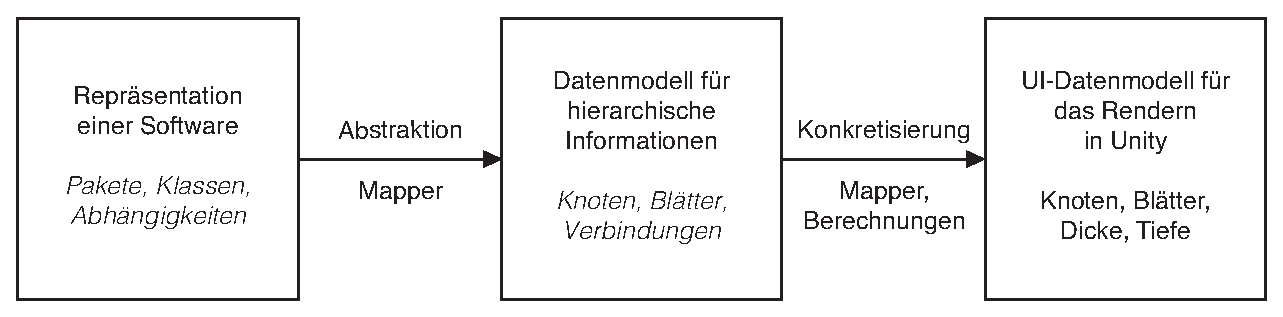
\includegraphics[width=\textwidth]{\figdir/data-layers}
  \caption{Schichten der Datenstrukturen}
  \label{fig:data-layers}
\end{figure}

\section{Software Meta-Modell}
\label{sec:software-model}

\subsubsection*{Vorhandene Meta-Modelle}

CodeCity verwendet als Meta-Modell für Software das sogenannte \textit{FAMIX}-Modell in Version 2.1. Dieses wird bis heute von \textit{Moose}, dem Software-Analyse-Tool, auf dem CodeCity basiert, protegiert und ist heut in Version 3.0 verfügbar und in \cite{merrill1916moose} beschrieben. Das Meta-Modell ist sehr umfangreich und beinhaltet 51 verschiedene Entities. Es wird in einem eigenen Dateiformat namens MSE, vergleichbar mit JSON, gespeichert. Da aber dynamische Informationen nicht im FAMIX-Modell enthalten sind, eignet sich das Format nicht um in CodeLeaves verwendet zu werden.

Ein Meta-Modell, das dynamische und statische Informationen vereint, existiert nach heutigem Wissensstand nicht.

Für eine reine dynamische Analyse ist das Tool \textit{ExplorVis} sehr ausgereift \cite{fittkau2017software}. Das im nachfolgende entwickelte Meta-Modell ist von Aspekten aus dem FAMIX- und dem ExplorVis-Modell inspiriert. Dabei soll das Modell aber möglichst simpel gehalten werden und nur das beinhalten, was CodeLeaves auch darstellen können soll.

\subsubsection*{Entwicklung eines eigenen Modells}

Um uns vor Augen zu führen, welche Informationen dargestellt werden können sollen, rufen wir uns die Userstories aus Kapitel \ref{ch:concept} in Erinnerung.

Aus den Userstories 1 und 4 ergeben sich folgende Informationen, die auch die Blattfarbe und damit auf jede Klasse angewandt werden können soll:

\begin{itemize}
  \item Statische Metriken zur Code-Qualität
  \item Antwortzeiten
  \item Laufzeitfehler
\end{itemize}

Eine \textit{Metric}-Entity ist also ein wichtiger Teil des Meta-Modells und wird mit einer \textit{Class}-Entity assoziiert. Mit einem Kompositum-Pattern mit der Class- und \textit{Paket}-Entity lässt sich die Struktur der Software beschreiben. Damit ist ein Teil von Userstory 3 abgedeckt.

Aus Userstory 1 und 3 lassen sich folgende mögliche Verbindungen ableiten:

\begin{itemize}
  \item Statische Abhängigkeiten
  \item Dynamische Aufrufe
\end{itemize}

Beide Verbindungen lassen sich im Meta-Modell als \textit{Assoziation}-Entity von einem Startpunkt zu einem Endpunkt modellieren. Statische Abhängigkeiten können sich unterscheiden. Es können Importe, Vererbungen, oder statische Aufrufe bzw. Zugriffe sein.

Durch die Expertengespräche ging hervor, dass sowohl bei Metriken wie Laufzeitfehler, als auch bei Verbindungen wie dynamische Aufrufe ein Bezug zum Code wichtig ist. Demnach müssen die Entities Association und Metric mindestens ein \textit{Codesnippet} beinhalten wo zum Beispiel der Fehler in der Klasse aufgetreten ist.

\todo{Association associated with class?}

Neben der Struktur, Metriken und den Verbindungen einer Software geht aus Userstory 1 hervor, dass es auch gilt die Ressourcen-Auslastung zu visualisieren. Diese Information wird parallel zu den bisher eingeführten Entities in der \textit{Utilization}-Entity gespeichert.

Damit sind bereits fast alle Informationen adressierbar. Es fehlt lediglich noch, dass der Wald auch zu unterschiedlichen Zeitpunkten bzw. Zeiträumen dargestellt werden kann. Dafür werden alle Informationen als Zeitreihe in einer \textit{Snapshot}-Entity gespeichert. So kann in der Zeit zurück gegangen werden und CodeLeaves kann somit auch die Evolution von Software unterstützen.

In Abbildung \ref{fig:meta-model} sind die Entities des entwickelten Meta-Modells zu sehen.

\begin{figure}[htb]
  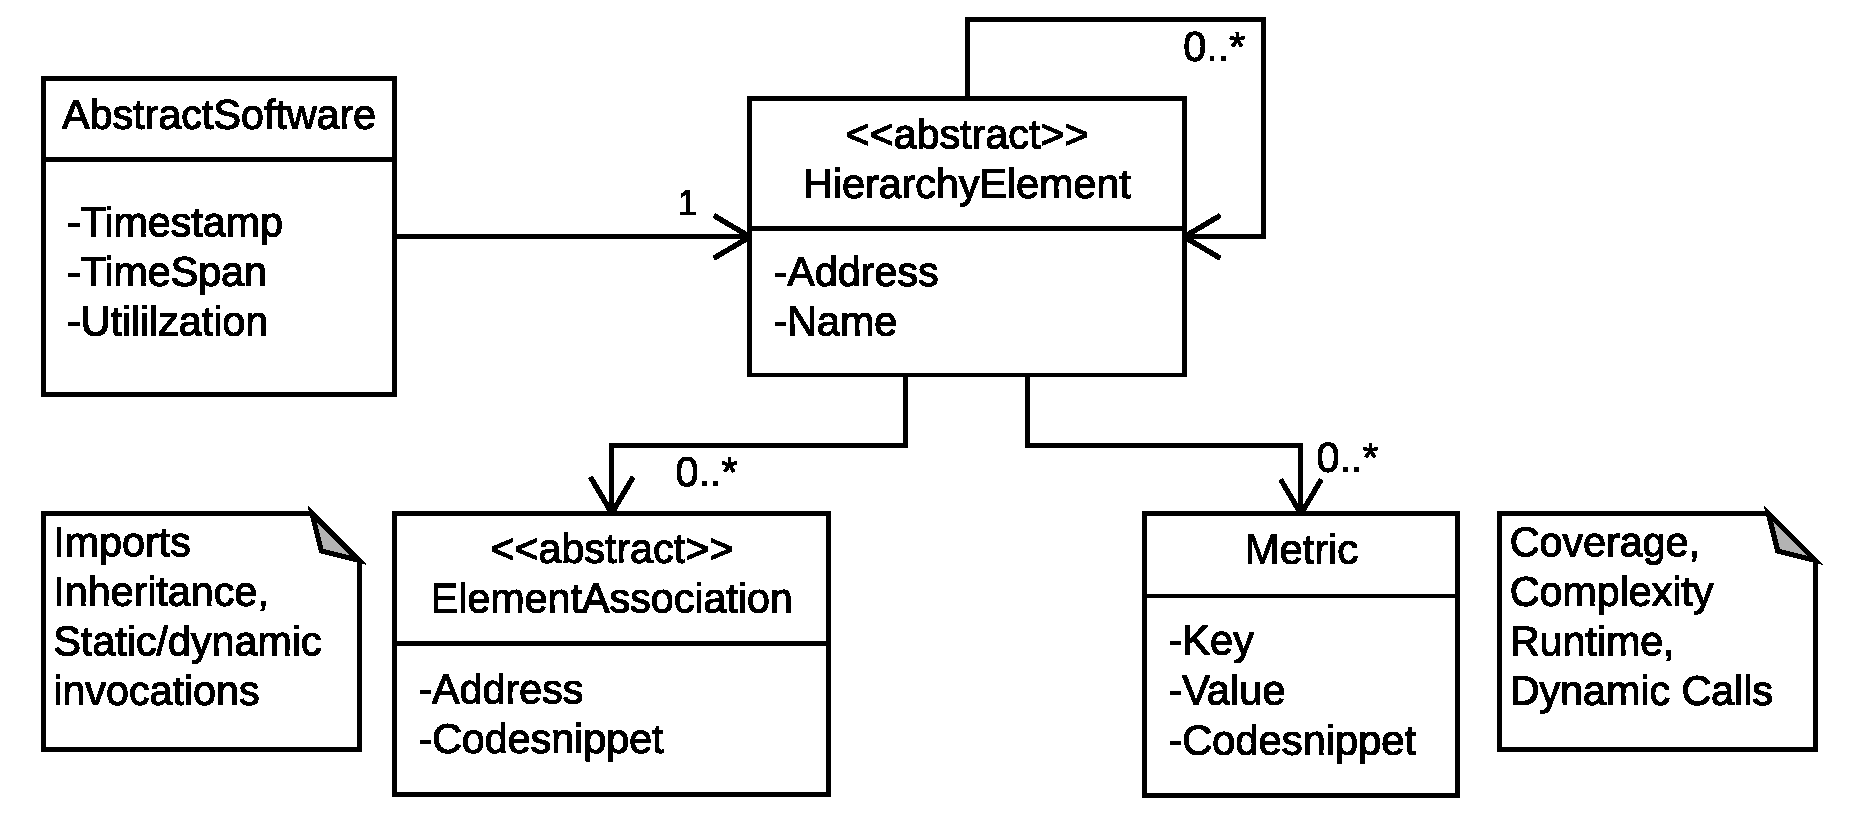
\includegraphics[width=\textwidth]{\figdir/meta-model}
  \caption{Meta-Modell einer Software}
  \label{fig:meta-model}
\end{figure}

Bei Betrachtung des Modells fällt auf, dass sich unter der Class-Entity noch die \textit{Method}-Entity befindet. Diese hat die gleichen Assoziationen wie de Class-Entity. Je nachdem was als Softwareartefakt festlegt wird, kann auf Klassen-Ebene aufgehört werden, oder aber noch weiter bis auf Methoden-Ebene vorgegangen werden. Die Assoziationen von der Class- und der Method-Entity sind gleich. Jede Metric- und Association-Entity lässt sich einer Class-Entity zuordnen, kann aber bei feinerer Granularität auch einer Method-Entity zugeordnet werden.

Im Rahmen dieser Arbeit wird als Softwareartefakt eine Klasse festgelegt. Das Modell wäre mit der Mehtod-Entity aber leicht auf Methoden-Ebene erweiterbar.

\section{Internes Datenmodell}
\label{sec:app-model}

\begin{figure}[htb]
  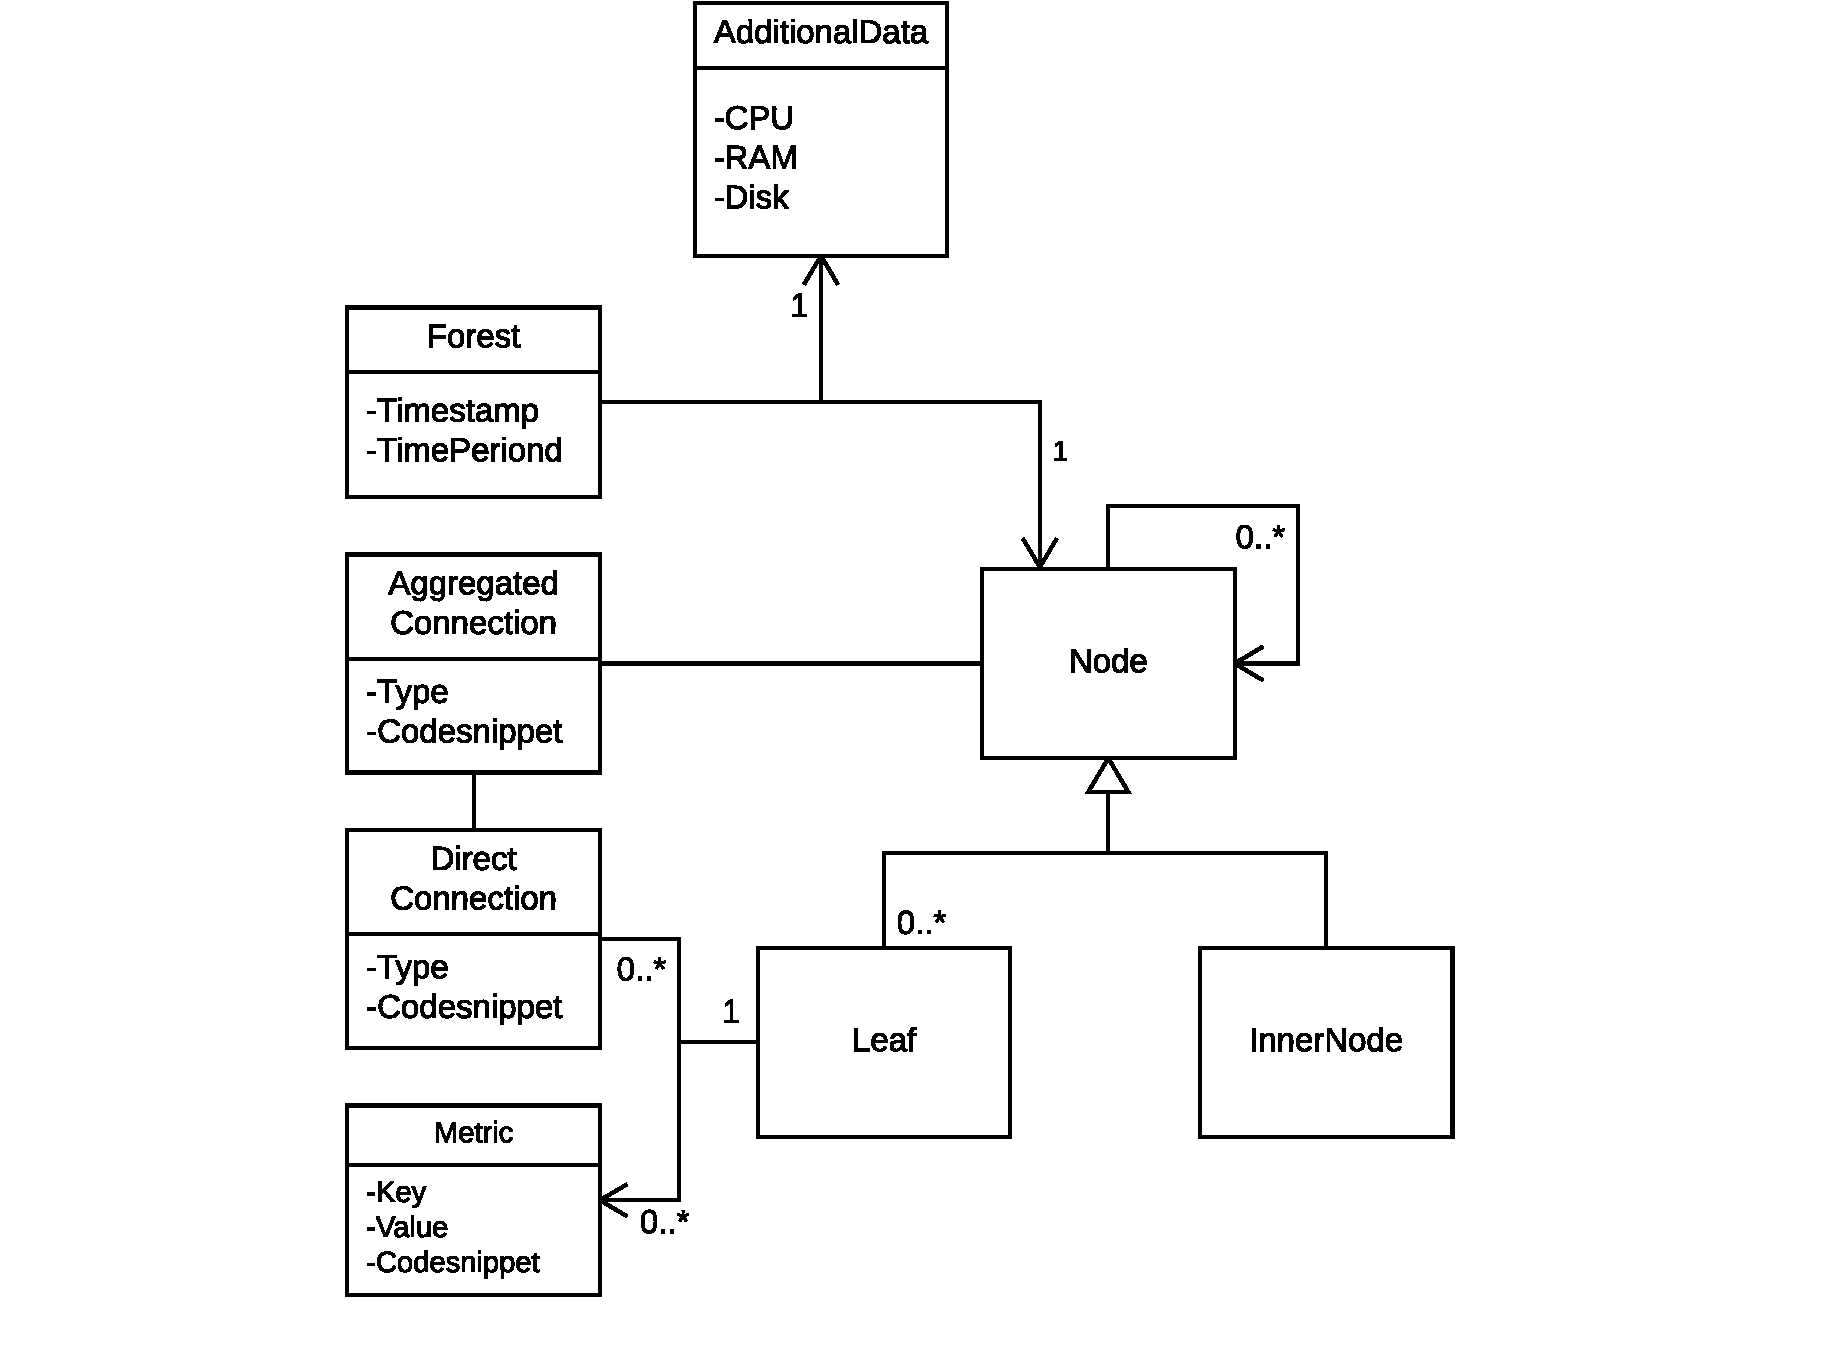
\includegraphics[width=\textwidth]{\figdir/internal-model}
  \caption{Internes Datenmodell}
  \label{fig:internal-model}
\end{figure}

\section{UI-Datenmodell}
\label{sec:hierarchical-model}

\begin{figure}[htb]
  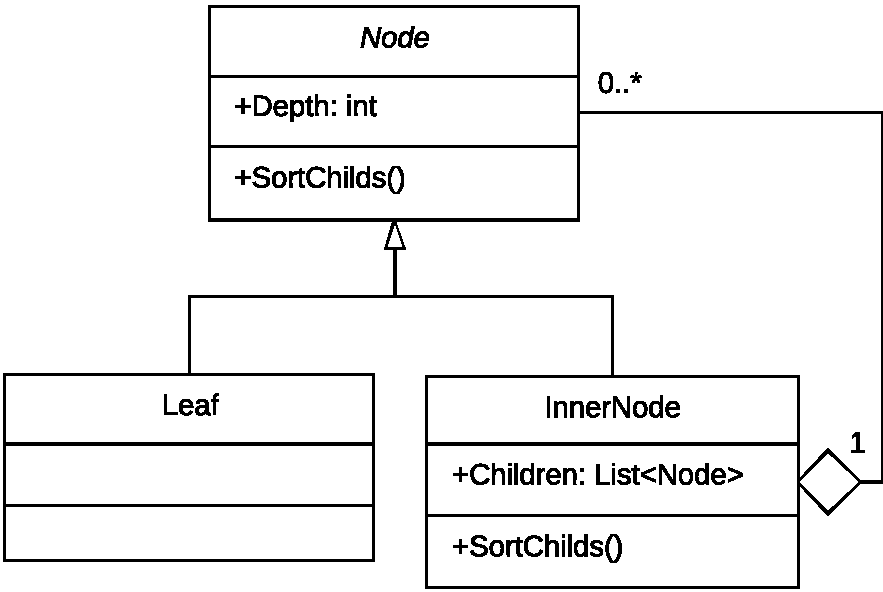
\includegraphics[width=.6\textwidth]{\figdir/ui-model}
  \caption{UI-Datenmodell}
  \label{fig:ui-model}
\end{figure}

% ----===== Chapter ====---- %
\chapter{Modellierung und Layout des Waldes}
\label{ch:layout}

\section{Grundlegender Ansatz}

CodeLeaves steht und fällt mit der korrekten und übersichtlichen Darstellung der Baumstruktur. Durch Akzeptanzkriterium \todo{link auf Akzeptanz} ist die Struktur der Bäume so zu generieren, dass so viele Blätter wie möglich gleichzeitig im Blickfeld des Betrachters ist. Auf der anderen Seite gilt es wegen Akzeptanzkriterium \todo{link auf Akzeptanz} die Struktur übersichtlich und deswegen mit so wenig Überschneidungen wie möglich zu generieren.

In Abschnitt \ref{sec:sunflower} und \ref{sec:circle-packing} werden deshalb zwei Algorithmen vorgestellt, die in Verbindung eine solche Darstellung der Baumstruktur ermöglicht. Für das Rendern in 3D müssen zunächst 3D Objekte entworfen werden, die die Knoten und Blätter repräsentieren. Dies wurde mithilfe der professionellen 3D Modellierungs-Software Maya\footnote{https://www.autodesk.de/products/maya/overview} von Audodesk erreicht.

\subsubsection*{3D Objekte}

Die Bäume für CodeLeaves kommen mit den Objekten Kante und Blatt aus. Ein innerer Knoten wird der Baum Metapher folgend immer durch die Kante zum Elternteil bzw. zum Waldboden dargestellt. Ein Blatt - im Sinne der Begriffsdefinition von Abschnitt \ref{sec:naming} - wird demnach vom dem dazugehörigen Blatt-Objekt und dem Kanten-Objekt zum Elternteil repräsentiert.

\paragraph{Kanten-Objekt} Eine Kanten-Objekt ist ein vertikal ausgerichteter, nach oben leicht zulaufender Zylinder was die Abbildung \ref{fig:edge} veranschaulicht. Die Pivots zur Position, Rotation und Skalierung wurden so gewählt, dass eine Manipulation des Objekts immer um den Mittelpunkt der Grundfläche der Kante erfolgt.\\

\paragraph{Blatt-Objekt} Das Blatt-Objekt wurde in Anlehnung an ein echtes Blatt modelliert und ist in Abbildung \ref{fig:leaf} zu sehen.\\

\setlength{\fwidth}{.3\textwidth}
\begin{figure}[htb]
  \centering
  \begin{subfigure}[b]{\fwidth}
   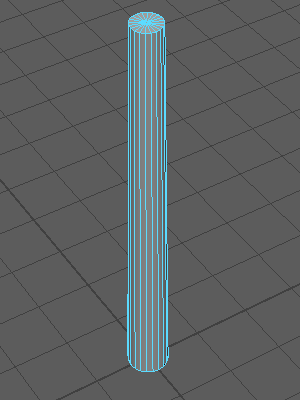
\includegraphics[width=\textwidth]{figures/edge}
   \subcaption{Kante} \label{fig:edge}
  \end{subfigure}
  \hspace{.5 cm}
  \begin{subfigure}[b]{\fwidth}
  	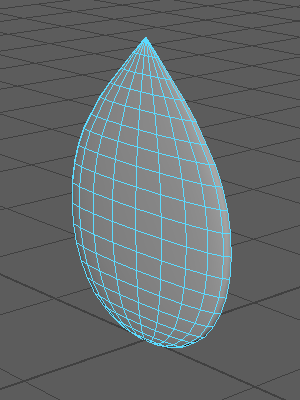
\includegraphics[width=\textwidth]{figures/leaf}
  	\subcaption{Blatt} \label{fig:leaf}
  \end{subfigure}
  \caption{3D Objekte für den Prototyp} \label{fig:3d-objects}
\end{figure}

Das Blatt-Objekt hat aufgrund der flachen Form die Eigenschaft, dass die sichtbare Fläche bei seitlicher Betrachtung deutlich geringer ist, als von vorne. Wir stellen uns einen Baum vor, bei dem der Betrachter nur die Kanten der Blätter sieht. Dadurch lassen sich die Farben der Blätter nur schwer miteinander vergleichen. Dies sollte aber aus jeder Postion möglich sein.

Eine Abhilfe könnte ein Blatt-Objekt sein, dass in allen Dimensionen gleich dick ist. Dies würde aber eher an eine Knospe erinnern und schaut wenig natürlich aus. Deshalb wird dem Blatt-Objekt in Unity eine Script hinzugefügt, dass das Blatt zur Laufzeit immer in die Richtung des Betrachters rotieren lässt. Ein 3D-Objekt mit einer solchen Verhalten wird \textit{Billboard} genannt. Mithilfe des Billboard-Verhaltens ist gewährleistet, dass der Nutzer von jedem Winkel aus immer eine optimale Übersicht über das Laubwerk besitzt.

\subsubsection*{Beschaffung von realistischen Beispieldaten}
Für die Generierung der Struktur im Prototyp wurde mit einem Beispielprojekt gearbeitet. Das Projekt lautet \textit{Air} und ist eines der größten Software-Projekte der QAware und wird seit rund 5 entwickelt.

In Tabelle \ref{tab:air} sind hinsichtlich der Struktur Eckdaten von Air angegeben.

\begin{table}[htb]
  \caption{Eckdaten des Beispielprojekts Air}\label{tab:air}
  \begin{tabular}{*{4}{D{2cm}}}
    Bäume & Knoten & Blätter & innere Knoten\\
    \hline
    40    & 6736   & 5373    & 1363 \\
  \end{tabular}
\end{table}

Alle Projekte von QAware werden in SonarQube überwacht. SonarQube bietet eine Web-API, durch die die Struktur eines Projekts und unterstützte statische Metriken abgefragt werden können. Diese API wird im Prototyp genutzt um die benötigten Informationen für Struktur der Software und Farben der Blätter abzufragen. Die Struktur wird zur Laufzeit rekursiv zusammengebaut, da SonarQube immer nur die direkten Kinder eines Softwareartefakts liefert.

Das Format von SonarQube wird dabei schon in das generische Software-Meta-Modell von CodeLeaves transferiert, was durch andere Daten später ergänzt werden kann. Da bei Air sehr viele HTTP-Requests entstehen, wird das entstandene Meta-Modell lokal in eine Datei geschrieben, sodass dieses als Beispiel-Datensatz für den Prototypen dient. Prinzipiell können aber auch dynamisch andere Projekte geladen werden.

Das Datenmodell des Backends wird in das Datenmodell der Application logic und weiter in das UI-Datenmodell transferiert.

Nun liegt eine Struktur vor, die es gilt zu Bäumen zusammen zu bauen. Der Grundlegende Ablauf des Algorithmus zur Generierung eines Baumes mit Kronenansatz $K$ und dessen Kindern $\lbrace(K_i) \mid i=1,2\hdots n\rbrace$ lässt sich wie folgt beschreiben:

\begin{enumerate}[(i), labelindent=0pt, align=left, itemsep=0pt, parsep=0pt, labelsep=.5em, leftmargin=!]
  \item Instanziiere eine Kante $E$ als Stamm des Baums.
  \item Falls Knoten $K$ ein Blatt ist, füge ein Blatt an $E$ an.
  \item Falls Knoten $K$ ein innerer Knoten ist ist, finde für jedes Kind $K_i$ eine passende Position, füge eine Kante $E_i$ zwischen $E$ und $K_i$ an, setze $K$ gleich $K_i$ und $E$ gleich $E_i$ und und geht zu (ii).
\end{enumerate}

Wie die Kinder eines Knotens sinnvoll verteilt werden, soll im Folgenden erarbeitet werden.

\subsubsection*{Verteilung von Kindern eines Elternteils}

Ein wichtiger Bestandteil der Modellierung von Bäumen ist die Verteilung der Kinder eines Knotens. Es stellt sich zunächst die Frage auf Grundlage welcher geometrischen Figur die Kinder verteilt werden. In Frage kommt eine Kugel und eine Kreisfläche.

\subsubsection*{Verteilung auf einer Kugel}
Werden die Kinder gleichmäßig auf der Oberfläche einer Kugel verteilt, wird der 3D Raum maximal ausgenutzt. Das Ergebnis käme einem \textit{Fractal tree} sehr nahe. Diese Bäume werden rekursiv durch die Neigung der Aststücke konstruiert. Ein solcher Fractal tree ist in Abbildung \ref{fig:fractal-tree} dargestellt. Das Konzept ließe sich problemlos in die Dreidimensionalität übertragen. Das Problem dabei ist, dass bei diesem Ansatz die Aststücke auch rekursiv verkürzt werden. Dadurch wird gewährleistet, dass die Äste nicht in den Boden wachsen.

Für CodeLeaves wären immer kleiner werdende Kanten wenig sinnvoll, da so eine Interaktion mit den kleiner werdenden Kanten und Blättern kaum möglich wäre. Auch die Überschneidungen, die in Abbildung \ref{fig:fractal-tree} zu sehen sind, wären bei größeren Bäumen nur durch Neigung der Kanten nicht zu vermeiden. Die Kollisionen, die dadurch im 3D Raum entstünden, würden sich negativ auf die Übersichtlichkeit der Bäume auswirken und müssen deswegen vermieden werden.

\begin{figure}[htb]
  
\includegraphics[width=.5\textwidth]{figures/fractal-tree}
  \caption{Fractal tree \cite{rocchini2017fractal}}
  \label{fig:fractal-tree}
\end{figure}

\subsubsection*{Verteilung auf einer Kreisfläche}
Werden die Kinder stattdessen auf gleicher Höhe auf einer Kreisfläche überhalb des Elternteils positioniert, muss die Länge der Kanten entsprechend angepasst werden. Dadurch entstehen drei Vorteile.

Erstens befinden sich Software-Artefakte mit der gleichen hierarchischen Tiefe auch auf gleicher Höhe, was sich positiv auf die Übersichtlichkeit auswirkt.

Zweitens wird das Laubdach primär am Ende des Baumes auf einer Ebene angezeigt, was aus der Vogelperspektive eine gute Betrachtung der Metriken verspricht und gleichzeitig von der Seite nicht den Blick auf die Struktur des Baumes versperrt.

Drittens kann durch die Längenanpassung der Kanten Kollisionen von Ästen vermieden werden. Der Abstand zischen zwei Geschwister muss so groß gewählt werden, dass die Kanten der Nachfahren beider Geschwister nicht miteinander kollidieren.\\

Der Prototyp von CodeLeaves verwendet aus genannten Gründen eine Kreisfläche für die Verteilung von Kinder eines Knotens.

\section{Verteilung von Blättern mit dem Sonnenblumen-Algorithmus}
\label{sec:sunflower}

Betrachten wir nun zunächst den einfachen Fall eines inneren Knotens, der nur Blätter als Nachfahren besitzt. D.h. die Verteilung kann gleichmäßig erfolgen und muss die Breite nachfolgender Knoten nicht mit einbeziehen.

Dieser Fall tritt in realen Softwareprojekten häufig auf. In Air existieren 1154 solcher Knoten, was $85\%$ aller inneren Knoten ausmacht. Nur $0,4\%$ aller inneren Knoten enthalten Blätter \textbf{und} weiter innere Knoten. Die Verteilung der Kinder eines Knotens mit inneren Knoten, wird im \ref{subsec:collision} behandelt.

\begin{quote}
  \textit{Es wird ein Algorithmus gesucht, bei dem Punkte auf einer Kreisfläche gleichmäßig verteilt werden.}
\end{quote}

Dazu liefert uns die Natur ein schönes Beispiel. Die kleinen inneren Blüten der Sonnenblume, die sogenannten Röhrenblüten, die nach Befruchtung die Sonnenblumenkerne ausbilden, nutzen den Platz innerhalb der gelben Zungenblüten optimal aus \cite{zimmermann2017sonnenblume}. Die spiralförmige Anordnung ist nicht nur ästhetisch, sondern folgt auch einem genauen Muster.

\begin{figure}[htb]
  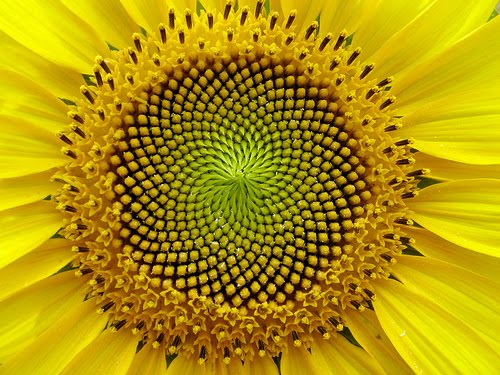
\includegraphics[width=.5\textwidth]{figures/sunflower-seeds}
  \caption{Spiralförmige Anordnung der Röhrenblüten einer Sonnenblume \cite{blender2017howto}}
  \label{fig:sunflower-seeds}
\end{figure}

\subsubsection*{Der Goldene Winkel}
Ausgehend von dem Mittelpunkt der Sonnenblume ist jede nachfolgender Blüte um rund 137.5 um den Mittelpunkt rotiert. Dieser sogenannte \textit{Goldener Winkel} entsteht durch die Teilung des Vollkreises durch den \textit{Goldenen Schnitt}. Der goldene Schnitt ist ein Teilungsverhältnis das oft bei Größenverhältnissen von einfachen geometrischen Figuren vorkommt und ist wie folgt definiert:

\begin{equation}
  \Phi = \frac{a}{b} = \frac{a + b}{a} = \frac{1 + \sqrt{5}}{2} \approx 1.618
\end{equation}

Wird der Vollwinkel durch den Goldenen Schnitt geteilt, entsteht folgender Winkel:

\begin{equation}
  \frac{2\pi}{\Phi} \approx \ang{222.5}
\end{equation}

Die Ergänzung zum Vollwinkel ist der Goldene Winkel:
\begin{equation}
  2\pi - \frac{2\pi}{\Phi} = \frac{2\pi}{\Phi^2} \approx \ang{137.5}
\end{equation}

Dieser hat die Eigenschaft, dass er aufaddiert nie den selben Winkel ergibt. Diese Eigenschaft machen sich viele Pflanzen zu Nutze und kann auch in CodeLeaves Anwendung finden.

\subsubsection*{Berechnungen für einen neuen Knoten}
Mit dem Vielfachen des goldenen Winkels ist der Winkel $\varphi$ gegeben, um den eine neue Kante um die y-Ache rotiert wird. Für die Rotation und Skalierung einer Kante sind aber noch andere Größen zu berechnen.

Wird eine Kante mit der Länge $l$ an einen Knoten angefügt, um die x-Achse mit dem Winkel $\theta$ geneigt und anschließend um die y-Achse mit den Winkel $\varphi$ rotiert, entsteht ein Kugelkoordinatensystem mit der Position des Elternteils als Ursprung $O$, der y-Achse als Polachse, der Position des $n$-ten Kindknoten als Punkt $P$, dem \emph{Polarwinkel} $\theta$ und dem \emph{Azimutwinkel} $\varphi$\cite{papula2001mathematik}.

\begin{figure}[htb]
  \tdplotsetmaincoords{60}{110}
%
\pgfmathsetmacro{\rvec}{1}
\pgfmathsetmacro{\thetavec}{30}
\pgfmathsetmacro{\phivec}{60}
%
\begin{tikzpicture}[scale=7,tdplot_main_coords]

\coordinate (O) at (0,0,0);
\draw[dashdotted,->] (0,0,0) -- (1,0,0) node[anchor=north east]{$z$};
\draw[dashdotted,->] (0,0,0) -- (0,1,0) node[anchor=north west]{$x$};
\draw[dashdotted,->] (0,0,0) -- (0,0,1) node[anchor=south]{$y$};

\tdplotsetcoord{P}{\rvec}{\thetavec}{\phivec}
\coordinate (E) at (Pz);

\draw[thick] (O) node[point,label=above left:$O$]{} -- node[left=3pt]{$h$} (E) node[point,label=above left:$E$]{};
\draw[thick] (O) -- node[below right]{$l$} (P) node[point,label=above right:$P$]{};
\draw (E) -- node[above right]{$a_n$} (P);
\draw[dashed] (O) -- (Pxy);
\draw[dashed] (P) -- (Pxy);
%\draw[dashed] (P) -- (Pyz);
%\draw[dashed] (E) -- (Pyz);

\tdplotsetthetaplanecoords{\phivec}
\tdplotdrawarc[tdplot_rotated_coords]{(E)}{0.1}{90}%
    {180}{above left}{$\cdot$}
\tdplotdrawarc{(O)}{0.2}{0}{\phivec}{anchor=north}{$\varphi$}
\tdplotdrawarc[tdplot_rotated_coords]{(0,0,0)}{0.3}{0}%
    {\thetavec}{anchor=south west}{$\theta$}
    
\end{tikzpicture}

%%Angle Definitions
%%-----------------
%
%%set the plot display orientation
%%synatax: \tdplotsetdisplay{\theta_d}{\phi_d}
%\tdplotsetmaincoords{0}{0}
%
%%define polar coordinates for some vector
%\pgfmathsetmacro{\rvec}{.8}
%\pgfmathsetmacro{\thetavec}{30}
%\pgfmathsetmacro{\phivec}{60}
%
%%start tikz picture, and use the tdplot_main_coords style to implement the display 
%%coordinate transformation provided by 3dplot
%\begin{tikzpicture}[scale=5, tdplot_main_coords]
%
%%set up some coordinates 
%%-----------------------
%\coordinate (O) at (0,0,0);
%
%%determine a coordinate (P) using (r,\theta,\phi) coordinates.  This command
%%also determines (Pxy), (Pxz), and (Pyz): the xy-, xz-, and yz-projections
%%of the point (P).
%%syntax: \tdplotsetcoord{Coordinate name without parentheses}{r}{\theta}{\phi}
%\tdplotsetcoord{P}{\rvec}{\thetavec}{\phivec}
%
%%draw figure contents
%%--------------------
%
%%draw the main coordinate system axes
%\draw[thick,->] (0,0,0) -- (1,0,0) node[anchor=north east]{$x$};
%\draw[thick,->] (0,0,0) -- (0,1,0) node[anchor=north west]{$y$};
%\draw[thick,->] (0,0,0) -- (0,0,1) node[anchor=south]{$z$};
%
%%draw a vector from origin to point (P) 
%\draw[-stealth,color=red] (O) -- (P);
%
%%draw projection on xy plane, and a connecting line
%\draw[dashed, color=red] (O) -- (Pxy);
%\draw[dashed, color=red] (P) -- (Pxy);
%
%%draw the angle \phi, and label it
%%syntax: \tdplotdrawarc[coordinate frame, draw options]{center point}{r}{angle}{label options}{label}
%\tdplotdrawarc{(O)}{0.2}{0}{\phivec}{anchor=north}{$\phi$}
%
%
%%set the rotated coordinate system so the x'-y' plane lies within the
%%"theta plane" of the main coordinate system
%%syntax: \tdplotsetthetaplanecoords{\phi}
%\tdplotsetthetaplanecoords{\phivec}
%
%%draw theta arc and label, using rotated coordinate system
%\tdplotdrawarc[tdplot_rotated_coords]{(0,0,0)}{0.5}{0}{\thetavec}{anchor=south west}{$\theta$}
%
%%draw some dashed arcs, demonstrating direct arc drawing
%\draw[dashed,tdplot_rotated_coords] (\rvec,0,0) arc (0:90:\rvec);
%\draw[dashed] (\rvec,0,0) arc (0:90:\rvec);

%set the rotated coordinate definition within display using a translation
%coordinate and Euler angles in the "z(\alpha)y(\beta)z(\gamma)" euler rotation convention
%syntax: \tdplotsetrotatedcoords{\alpha}{\beta}{\gamma}
%\tdplotsetrotatedcoords{\phivec}{\thetavec}{0}

%translate the rotated coordinate system
%syntax: \tdplotsetrotatedcoordsorigin{point}
%\tdplotsetrotatedcoordsorigin{(P)}

%use the tdplot_rotated_coords style to work in the rotated, translated coordinate frame
%\draw[thick,tdplot_rotated_coords,->] (0,0,0) -- (.5,0,0) node[anchor=north west]{$x'$};
%\draw[thick,tdplot_rotated_coords,->] (0,0,0) -- (0,.5,0) node[anchor=west]{$y'$};
%\draw[thick,tdplot_rotated_coords,->] (0,0,0) -- (0,0,.5) node[anchor=south]{$z'$};

%WARNING:  coordinates defined by the \coordinate command (eg. (O), (P), etc.)
%cannot be used in rotated coordinate frames.  Use only literal coordinates.  

%draw some vector, and its projection, in the rotated coordinate frame
%\draw[-stealth,color=blue,tdplot_rotated_coords] (0,0,0) -- (.2,.2,.2);
%\draw[dashed,color=blue,tdplot_rotated_coords] (0,0,0) -- (.2,.2,0);
%\draw[dashed,color=blue,tdplot_rotated_coords] (.2,.2,0) -- (.2,.2,.2);

%show its phi arc and label
%\tdplotdrawarc[tdplot_rotated_coords,color=blue]{(0,0,0)}{0.2}{0}{45}{anchor=north west,color=black}{$\phi'$}

%change the rotated coordinate frame so that it lies in its theta plane.
%Note that this overwrites the original rotated coordinate frame
%syntax: \tdplotsetrotatedthetaplanecoords{\phi'}
%\tdplotsetrotatedthetaplanecoords{45}

%draw theta arc and label
%\tdplotdrawarc[tdplot_rotated_coords,color=blue]{(0,0,0)}{0.2}{0}{55}{anchor=south west,color=black}{$\theta'$}

%\end{tikzpicture}

%\end{document}
  \caption{Kugelkoordinatensystem mit den zu berechnenden Größen für das Hinzufügen eines neuen Knotens}
  \label{fig:spherical-coordinates}
\end{figure}

Diese Größen sind in Abbildung \ref{fig:spherical-coordinates} dargestellt, wobei die Höhe $h$ als Standardhöhe einer Kante gegeben gilt und $E$ mit $(0, h, 0)$ die Position des $0$-ten Kindes ist.

Der Abstand $d_n$ zwischen dem Punkt $E$ und $P$ berechnet sich für den $n$-ten Knoten nach \cite{vogel1979better} mit

\begin{equation}
\label{eq:r}
  d_n = c \sqrt{n},
\end{equation}

wobei $c$ eine Konstante ist und den Abstand der Kindknoten untereinander beeinflusst.

Die Rotation um die y-Achse $\varphi$ ist wie oben hergeleitet das $n$-te Vielfache vom Goldenen Winkel:

\begin{equation}
  \varphi = \frac{2\pi \cdot n}{\Phi^{2}}
\end{equation}

Der Polwinkel $\theta$ lässt sich mithilfe von $h$ und $r$ berechnen.

\begin{equation}
  \theta = tan^{-1} \left(\frac{r}{h}\right)
\end{equation}

Für die Positionierung des Kindknotens muss der Punkt $P$ von den Kugelkoordinaten $(l, \theta, \varphi)$ in das kartesische Koordinatensystem umgerechnet werden. Dies wird durch folgende Formel erreicht:

\begin{equation}
  \vv{P} =
  \begin{pmatrix}
    \sin\left(\varphi\right) \cdot \sin\left(\theta\right) \cdot l\\
    \cos\left(\theta\right) \cdot l\\
    \cos\left(\varphi\right) \cdot \sin\left(\theta\right) \cdot l
  \end{pmatrix}
\end{equation}

Damit ist alles für den Algorithmus gegeben, der Kinder eines Knotens mit gleichmäßigem Abstand auf eine gegebene Höhe verteilt und die Kanten entsprechend rotieren und skalieren kann

In Unity und C\# ist dieser Algorithmus in vereinfachter Form in Listing \ref{lst:addnode} zu sehen ist.

\begin{codesnippet}{Hinzufügen von Kinder eines Knotens}{lst:addnode}
for (var i = 0; i < node.Children.Count; i++)
{
    var d = TreeGeometry.CalcDistance(i);
    var phi = TreeGeometry.CalcPhi(i);
    var theta = TreeGeometry.CalcTheta(DefaultEdgeHeight, r);
    var l = TreeGeometry.CalcEdgeLength(DefaultEdgeHeight, theta);
    var pVec = TreeGeometry.CalcNodePosition(l, theta, phi);

    AddEdgeObject(l, theta, phi);
    AddEmptyNodeObject(pVec);
}
\end{codesnippet}

Das Ergebnis ist in Abbildung \ref{fig:sunflower-algorithm} zu sehen. Auf der linken Seite (\ref{fig:sunflower-30}) sind 30 Blätter verteilt worden. Die Ähnlichkeit zur Verteilung der Röhrenblüten der Sonnenblume wird auf der rechen Seite (\ref{fig:sunflower-200}) mit der Extremsituation mit 200 Blättern und kleinem $c$ sichtbar.

\setlength{\fwidth}{.49\textwidth}
\begin{figure}[htb]
  \centering
  \begin{subfigure}[b]{\fwidth}
   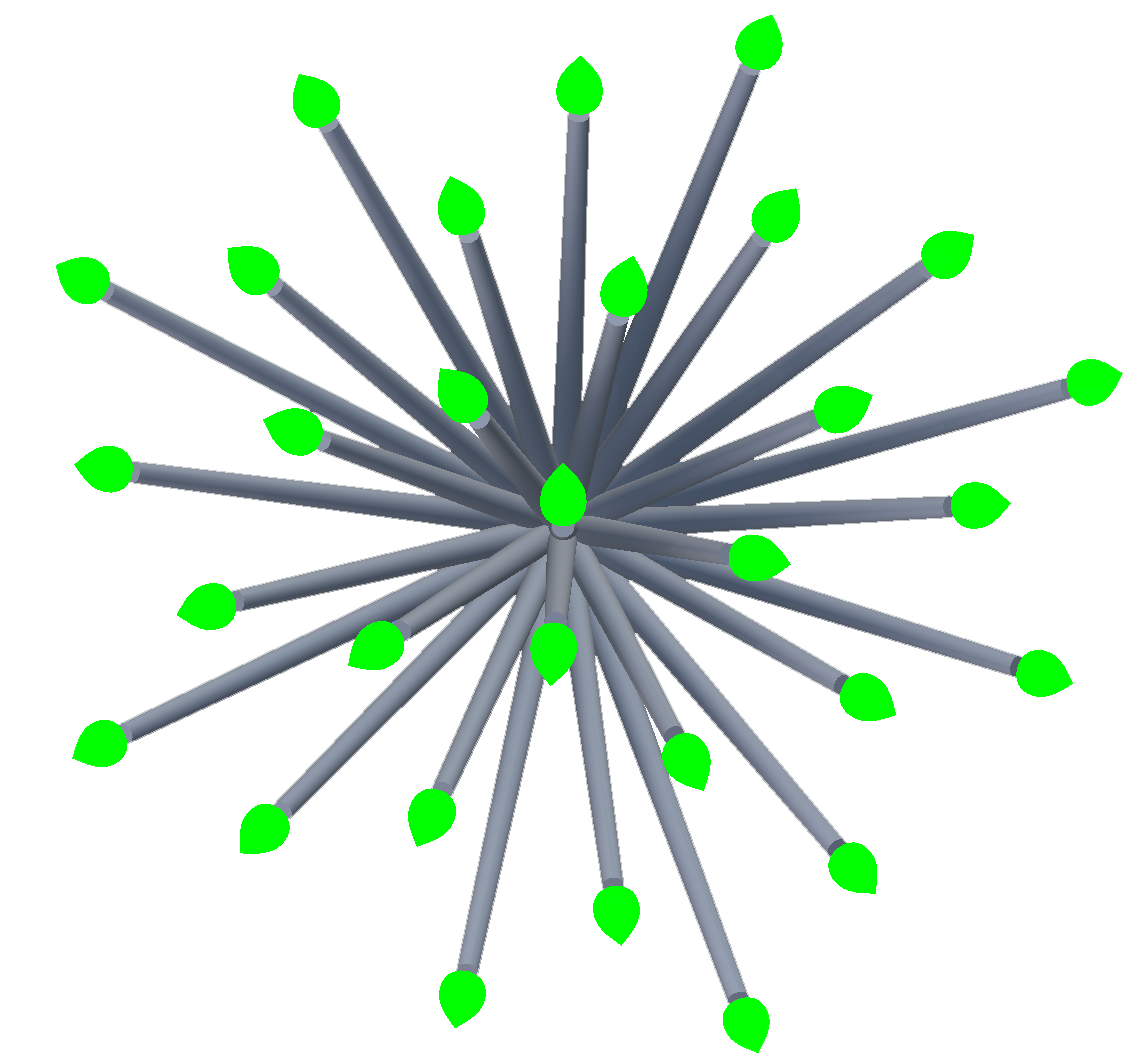
\includegraphics[width=\textwidth]{figures/sunflower-30_2}
   \subcaption{30 Blätter mit $c = 0.05$} \label{fig:sunflower-30}
  \end{subfigure}
  \hfill
  \begin{subfigure}[b]{\fwidth}
  	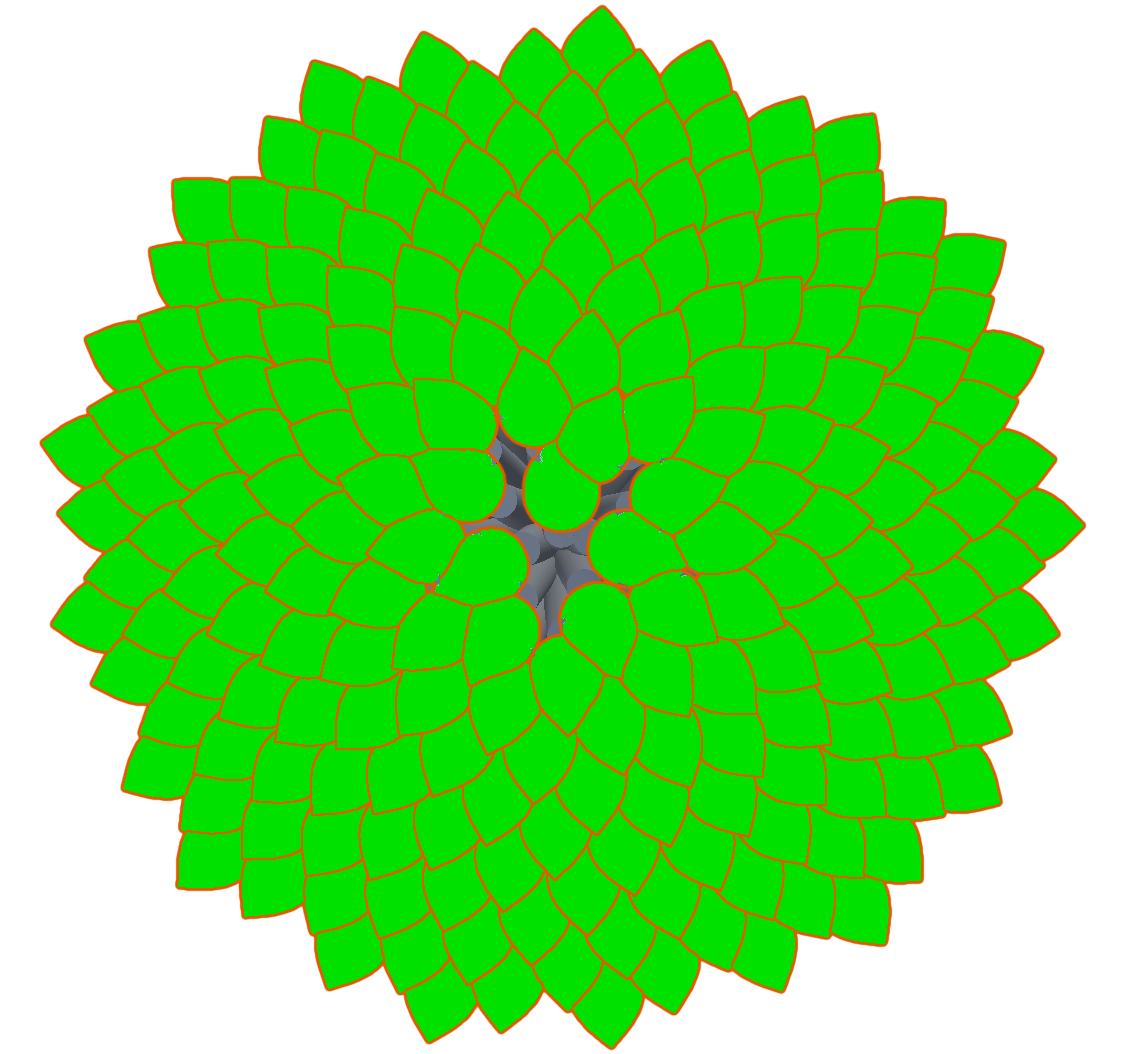
\includegraphics[width=\textwidth]{figures/sunflower-200}
  	\subcaption{200 Blätter mit $c = 0.01$} \label{fig:sunflower-200}
  \end{subfigure}
  \caption{Sonnenblumen-Algorithmus zur Verteilung von Blättern} \label{fig:sunflower-algorithm}
\end{figure}

\section{Verteilung innerer Knoten mit Circle-Packing}
\label{sec:circle-packing}

Die Verteilung mit dem Sonnenblumen-Algorithmus beruht auf der Tatsache, dass die Kinder des Knotens mit gleichmäßigem Abstand zueinander verteilt werden können. Dies ist bei inneren Knoten, die wiederum innere Knoten als Kinder besitzen, nicht gegeben. In diesem Fall muss die Breite der Kinder mit berücksichtigt werden, sodass die Äste der einzelnen Kinder nicht kollidieren.

Für die Verteilung der inneren Knoten mit einer minimalen Höhe von 1, führen wir ein weiteres Merkmal ein.

\begin{defbox}{Kreis und Radius eines inneren Knotens}{radius}
   Der Radius eines inneren Knotens ist der Radius des Kreises, aus dem alle Nachfahren des Knotens von oben betrachtet nicht hinaus ragen.
\end{defbox}

Bei einem inneren Knoten, dessen Kinder nach dem Sonnenblumen-Algorithmus verteilt wurden, kann dessen Radius leicht berechnet werden. Der Radius $r$ des inneren Knoten ist gleich dem Abstand $a_n$ des $n$-ten Kindes, der nach Formel \ref{eq:r} mit $a_n = c \sqrt{n}$ berechnet werden kann.

Werden nun alle inneren Knoten so verteilt, dass sich von oben betrachtet die Kreise der Kinder nicht überschneiden, sind alle Äste eines Baumes kollisionsfrei verteilt und alle Blätter sind von oben sichtbar.

Das Problem der Verteilung von inneren Knoten kann demnach auf 2D reduziert werden.\\

\textit{Es wird ein Algorithmus gesucht, der Kreise unterschiedlicher Größe auf möglichst kleinem Raum überschneidungsfrei positioniert.}\\

Diese Aufgabenstellung wird vom sogenannten \textit{Circle-Packing} gelöst.

Dazu hat Wang in \cite{wang2006visualization} 2006 einen Algorithmus entworfen, der seitdem von vielen adaptiert worden ist. Zum Beispiel in der populären JavaScript Library \textit{d3.js} zur Datenvisualisierung verwendet Bostock, der Schöpfer von d3.js diesen Algorithmus \cite{bostock2017abetter}.

Der Algorithmus muss noch an die Gegebenheiten von CodeLeaves angepasst werden. Bei Wang's Version startet der Algorithmus bereits mit drei tangentialen Kreisen. Der Mittelpunkt, um den zusätzliche Kreise positioniert werden, befindet sich zwischen den drei initialen Kreisen. Bei CodeLeaves sind aber nicht zwangsläufig bei jedem Knoten mindestens drei Kindknoten zu verteilen und als Mittelpunkt für die Verteilung der Kreise ist der Mittelpunkt des $0$-ten Kreises sinnvoll, da sich so immer ein Hauptstamm für einen Baum ergibt.

Ist nur ein Knoten zu verteilen, wird der Mittelpunkt seines Kreises von oben gesehen (in der XZ-Ebene) in den Ursprung gelegt. Der Kreis eines zweiten Knotens wird in einem zufälligen Winkel tangential zum Kreis des ersten Knotens positioniert. Bereits bei einem dritten Kreis kann Wangs's Algorithmus Anwendung finden.

Es wird eine sogenannte \textit{Front-Chain} verwendet, eine zyklische Liste, die alle Kreise enthält, an die potentiell ein neuer Kreis angefügt werden könnte. Die Front-Chain ist in Abbildung \ref{fig:circle-packing} als dickere Linie dargestellt. Bei der Positionierung des ersten bzw. des zweiten Kreises werden diese zur Front-Chain hinzugefügt.

Im Ganzen ist der leicht modifizierte Algorithmus für eine Menge von Kreisen $\lbrace C_i \mid i = 1, 2 \cdots n \rbrace$ im Folgenden beschrieben:

\subsubsection*{Abgewandelte Form von Wang's Circle-Packing-Algorithmus (nach \cite{wang2006visualization})}

\begin{enumerate}[(i), labelindent=0pt, align=left, itemsep=0pt, parsep=0pt, labelsep=.5em, leftmargin=!]
  \item Falls $n >= 1$ setzte den Mittelpunkt von $C_0$ in den Ursprung und füge $C_0$ zur Front-Chain hinzu.
  \item Falls $n >= 2$ setzte den Mittelpunkt von $C_1$ so, dass $C_1$ in einem zufälligen Winkel tangential zu $C_0$ ist und füge $C_1$ zur Front-Chain hinzu.
  \item Für $1 < i < N$ suche $C_m$, der Kreis dessen Mittelpunkt am nächsten zum Ursprung ist. $C_n$ ist der Kreis in der Front-Chain nach $C_m$.
  \item Berechne den Mittelpunkt von $C_i$ so, dass er tangential zu $C_m$ und $C_n$ ist.
  \item Suche einen Kreis $C_j$ der sich mit $C_i$ überschneidet.
  \item Falls der $C_j$ nicht existiert, setze $C_i$ gleich $C_{i+1}$ und gehe zu (iii).
  \item Falls $C_j$ in der Front-Chain näher an $C_m$ als an $C_n$ ist, lösche alle Kreise aus der Front-Chain, die zwischen $C_j$ und $C_n$ liegen. Setze $C_m$ gleich $C_j$ und gehe zu (iv).
  \item Falls $C_j$ in der Front-Chain näher an $C_n$ als an $C_m$ ist, lösche alle Kreise aus der Front-Chain, die zwischen $C_m$ und $C_j$ liegen. Setze $C_n$ gleich $C_j$ und gehe zu (iv).
\end{enumerate}

\label{subsec:collision}\setlength{\fwidth}{.4\textwidth}
\begin{figure}[htb]
  \captionsetup{justification=centering}
  \begin{subfigure}[t]{\fwidth}
   
\includegraphics[width=150px]{figures/add-circle}
   \subcaption{Platzieren eines neuen Kreises} \label{fig:add-circle}
  \end{subfigure}
  \hspace{1cm}
  \begin{subfigure}[t]{\fwidth}
  	
\includegraphics[width=150px]{figures/update-frontchain}
  	\subcaption{Anpassung der Front-Chain und erneutes Platzieren} \label{fig:update-frontchain}
  \end{subfigure}
  \caption{Wang's Circle Packing Algorithmus (nach \cite{bostock2017abetter})}
  \label{fig:circle-packing}
\end{figure}

In Abbildung \ref{fig:circle-packing} ist ein Ausschnitt aus dem Algorithmus visualisiert. Auf der linken Seite (\ref{fig:add-circle}) ist Schritt (iv) dargestellt, wobei $C_j$ existiert und und näher an $C_m$, als an $C_n$ liegt. Demnach werden alle Knoten zwischen $C_j$ und $C_n$ aus der Front-Chain entfernt und $C_i$ wird erneut platziert. Das Resultat ist auf der rechten Seite (\ref{fig:update-frontchain}) zu sehen.

Werden die Knoten vor der Durchführung des Algorithmus nach deren Radien sortiert, befindet sich der Knoten mit dem größten Kreis genau über dem Stamm und nach außen hin werden die Äste kleiner, was einem natürlichem Wuchs am nächsten kommt. Durch die zufällige Positionierung des $1$-ten Knotens, wächst der Baum nicht bei jedem Knoten "`in die gleiche Richtung"' was das natürliche Bild des Waldes ebenfalls fördert.

Der oben beschriebene Algorithmus setzt in (ii) und in (iv) die Berechnung eines Mittelpunktes voraus, sodass dessen Kreis tangential zu einem bzw. zwei weiteren Kreisen ist.

Bei dem $1$-ten Kreis mit Radius $r_1$ und Mittelpunkt $M_1$, der nur tangential zu dem $0$-ten Kreis mit $r_0$ und $M_0 = (0,0)$ ist und mit dem zufälligen Winkel Polarwinkel $\alpha$ platziert wird, ergibt sich für die XZ-Ebene folgende Koordinate:

\begin{equation}
  \vv{M}_1 =
  \begin{pmatrix}
    x = \cos\left(\alpha\right) \cdot \left(r_1 + r_2\right)\\
    y = \sin\left(\alpha\right) \cdot \left(r_1 + r_2\right)\\
  \end{pmatrix}
\end{equation}

Bei allen weitern Kreisen $C_i$ ist die Berechnung komplexer. Der Sachverhalt ist in Abbildung \ref{fig:tangent-circle} abgebildet. Gesucht ist $M_3$. Gegeben sind die Mittelpunkte $M_1$ und $M_2$ sowie die Radien der drei Kreise.

\begin{figure}[htb]
  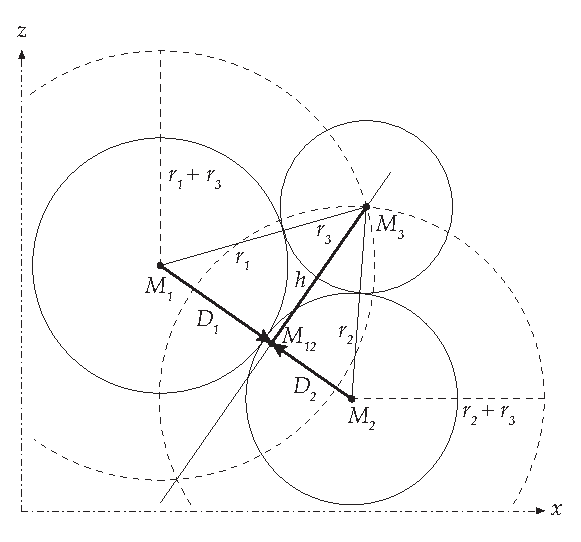
\includegraphics[width=261.593px]{figures/tangent-circle}
  \caption{Berechnung der Position eines Kreises, tangent zu zwei anderen Kreisen}
  \label{fig:tangent-circle}
\end{figure}

$M_3$ befindet sich genau an einem Schnittpunkt der beiden Kreise $\lbrace X \in XZ \mid \overline{M_1 X} = r_1 + r_3 \rbrace$ und $\lbrace X \in XZ \mid \overline{M_2 X} = r_2 + r_3 \rbrace$, die in Abbildung \ref{fig:tangent-circle} gestrichelt veranschaulicht sind. Diese Schnittpunkte lassen sich mithilfe von Vektorrechnung wie folgt errechnen:

\begin{equation}
  \vv{M}_{3_{1/2}} = \vv{M}_1 + \vv{D}_{1} \pm h \cdot \vv{e}
\end{equation}

Dabei ist $e$ ein zu $M_2 - M_1$ orthogonaler Einheitsvektor, für $h$ gilt

\begin{equation}
\label{equ:h}
  h = \sqrt{r_1^2 - \vert d_1 \vert^2} = \sqrt{r_2^2 - \vert d_2 \vert^2}
\end{equation}

und $D_1$ lässt sich durch Umformen der Gleichung \ref{equ:h} mit

\begin{equation}
  \vv{D}_1 = \frac{1}{2} \cdot \left( \frac{r_1^2 - r_2^2}{\vert \vv{M}_2 - \vv{M}_1 \vert} + 1 \right)
\end{equation}

darstellen.

Mit diesen Gleichungen kann der Circle-Packing Algorithmus für Kinder eines Knotens angewandt werden. Für die Positionierung der Knoten im dreidimensionalen Raum kommt für die Y-Koordinate jeweils noch die Länge der Kante des $0$-ten Geschwisters hinzu. Die Kanten der Geschwister müssen entsprechend deren Position angepasst werden

\subsubsection*{Knoten mit gemischten Kindern}

Für den Fall, dass ein Paket innere Knoten \textbf{und} Blätter enthält, kann der Circle-Packing-Algorithmus ebenfalls angewandt werden. Dafür muss lediglich einem Blatt ein Radius zugewiesen werden. Mit der Verwendung der Konstante $c$ aus dem Sonnenblumen-Algorithmus als Radius, haben die Blätter bei beiden Verteilungs-Algorithmen den gleichen Abstand zueinander. Lediglich die Ausbreitung der Blätter um den Ursprung erfolgt weniger natürlich, als beim Sonnenblumen-Algorithmus.

\subsubsection*{Hierarchische Anwendung}

Für die Anwendung auf mehreren Ebenen ist nach der Verteilung von Kindern eines Knotens $K$ auf Ebene $n$ die Berechnung des Radius von $K$ nötig, dass in Ebene $n - 1$ die Generation von $K$ verteilt werden kann.

Der Radius des Kreises von Knoten $K$ (mit Mittelpunkt an der Position von $K$), der alle Kreise der Kinder von $K$ umschließt und mindestens zu einem Kreis der Kinder tangential ist, ist der Abstand vom $0$-ten Kind zum $n$-ten Kind zuzüglich des Radius des $n$-ten Kindes. Diese Methode ist nicht der kleinste umschließende Kreis, reicht für die Generierung von überschneidungsfreien Bäume jedoch aus. Wir nennen den Kreis dieser Methode den \textit{größten umschließenden Kreis}.

Für die vollständige hierarchische Anwendung des Circle-Packing wird für jeden Knoten rekursiv das Circle-Packing durchgeführt und anschließend der eigene Radius gesetzt. Abbruchbedingung für die Rekursion ist, dass der Knoten ein Blatt, oder ein innerer Knoten mit ausschließlich Blättern ist. In letzterem Fall greift der Sonnenblumen-Algorithmus.

Das heißt der Algorithmus fängt mit dem Knoten mit der größten Tiefe an und arbeitet sich über Geschwister und Elternteile bis hin zum Kronenansatz fort, bis alle Knoten eines Baumes verteilt sind.

\subsubsection*{Verteilung von Bäumen}

Die Verteilung der einzelnen Bäume kann durch das Circle-Packing sehr leicht umgesetzt werden. Nachdem der Kronenansatz einen Radius besitzt, ist damit auch die Radius des ganzen Baumes bekannt. Damit können die Bäume beliebig platziert werden, ohne dass sich deren Äste überschneiden würden. Es wäre zum Beispiel eine Verteilung in einem Gitter möglich, was dann an eine Baumschule mit Baumreihen erinnern würde. Es ist jedoch auch ganz einfach möglich die Bäume ebenfalls mit Circle-Packing anzuordnen. Damit entsteht ein runder Wald und die Bäume nehmen möglichst wenig Platz ein.

Mit den beiden beschriebenen Algorithmen können Bäume garantiert überschneidungsfrei generiert und verteilt werden. Ein Auszug aus einem so entstanden Wald ist von der Seite in Abbildung \ref{fig:layout} und von oben in \ref{fig:circle-packing-code-leaves} zu sehen. Die Kreise in Abbildung \ref{fig:circle-packing-code-leaves} sind die Visualisierungern der durch das Circle-Packing entstehenden Kreise. Aus der Vogelperspektive ist gut zu erkennen, wie die Blätter innerhalb ihrer Eltern mithilfe des Sonnenblumen-Algorithmus sehr gleichmäßig verteilt werden.

%\begin{figure}[htb]
%  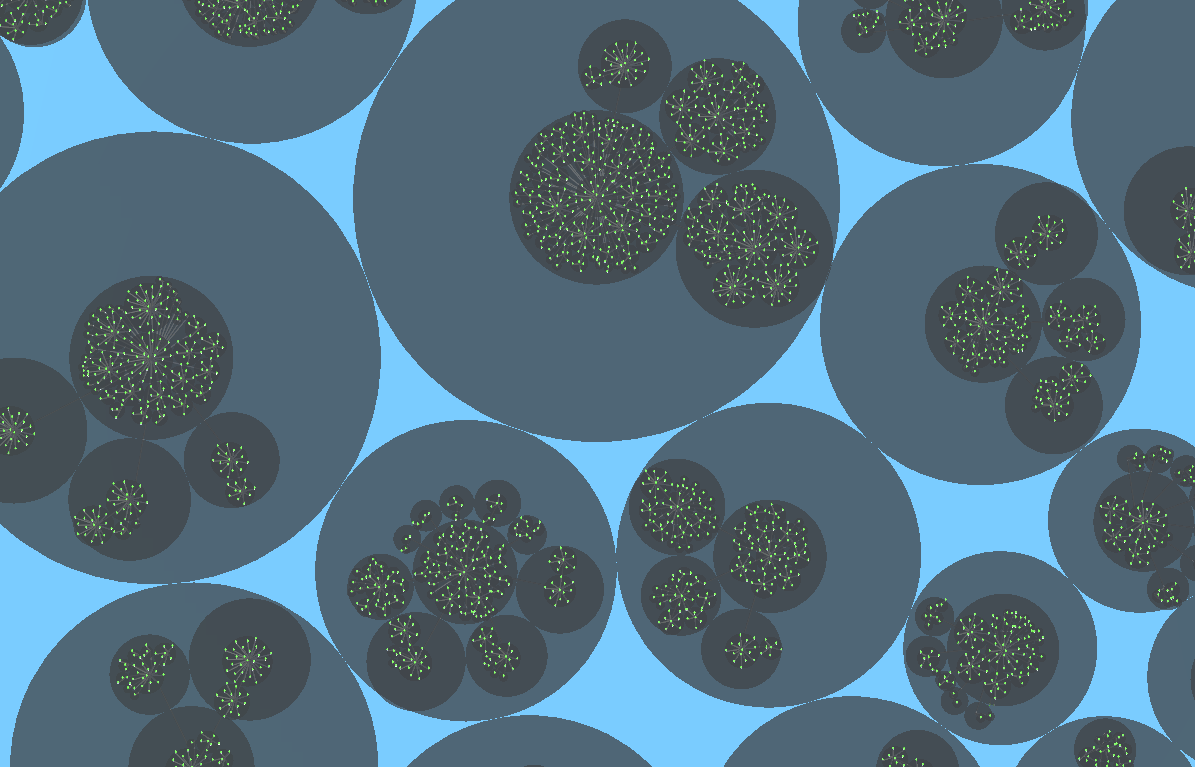
\includegraphics[width=\textwidth]{figures/circle-packing}
%  \caption{Circle-Packing in CodeLeaves}
%  \label{fig:circle-packing-code-leaves}
%\end{figure}
%
%\begin{figure}[htb]
%  \includegraphics[width=\textwidth]{figures/forest-structure}
%  \caption{Circle-Packing in CodeLeaves}
%  \label{fig:layout}
%\end{figure}

\begin{figure}[htb]
  \centering
  \begin{subfigure}[t]{\textwidth}
    \centering
    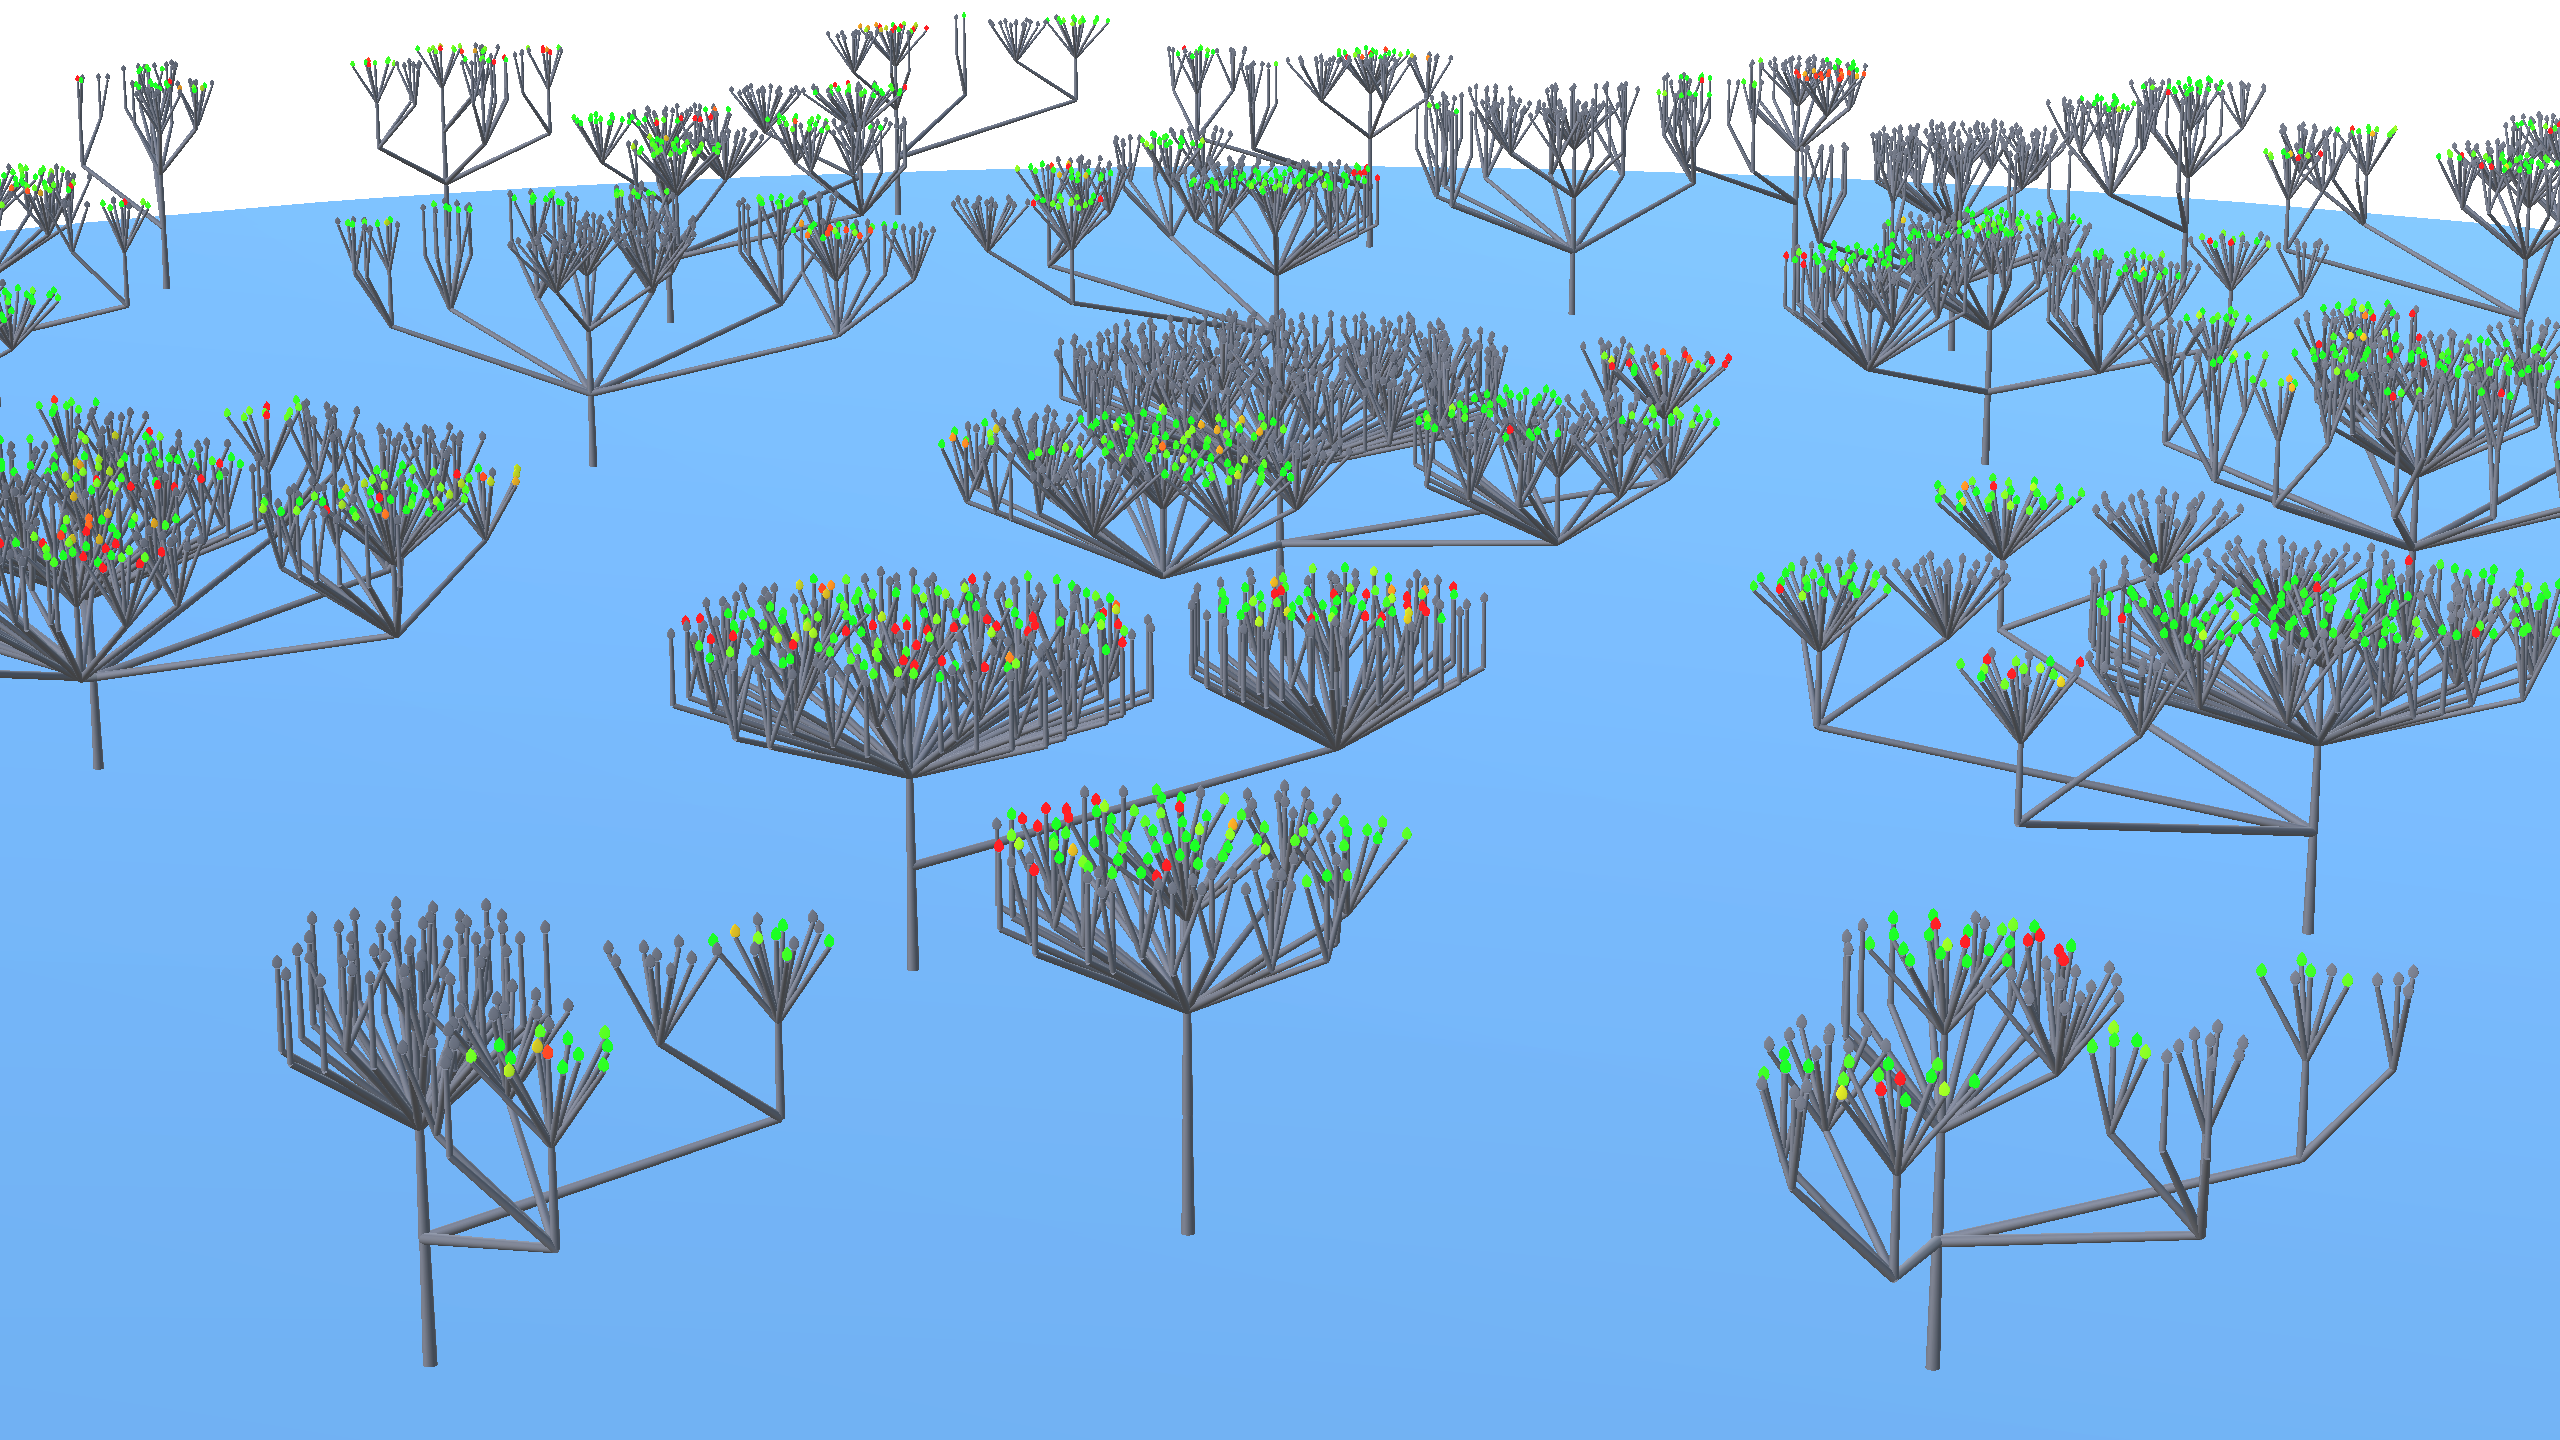
\includegraphics[width=\textwidth]{figures/layout-3}
    \subcaption{Seitenansicht} \label{fig:project-selection}
  \end{subfigure}
  \par\bigskip
  \begin{subfigure}[t]{\textwidth}
    \centering
  	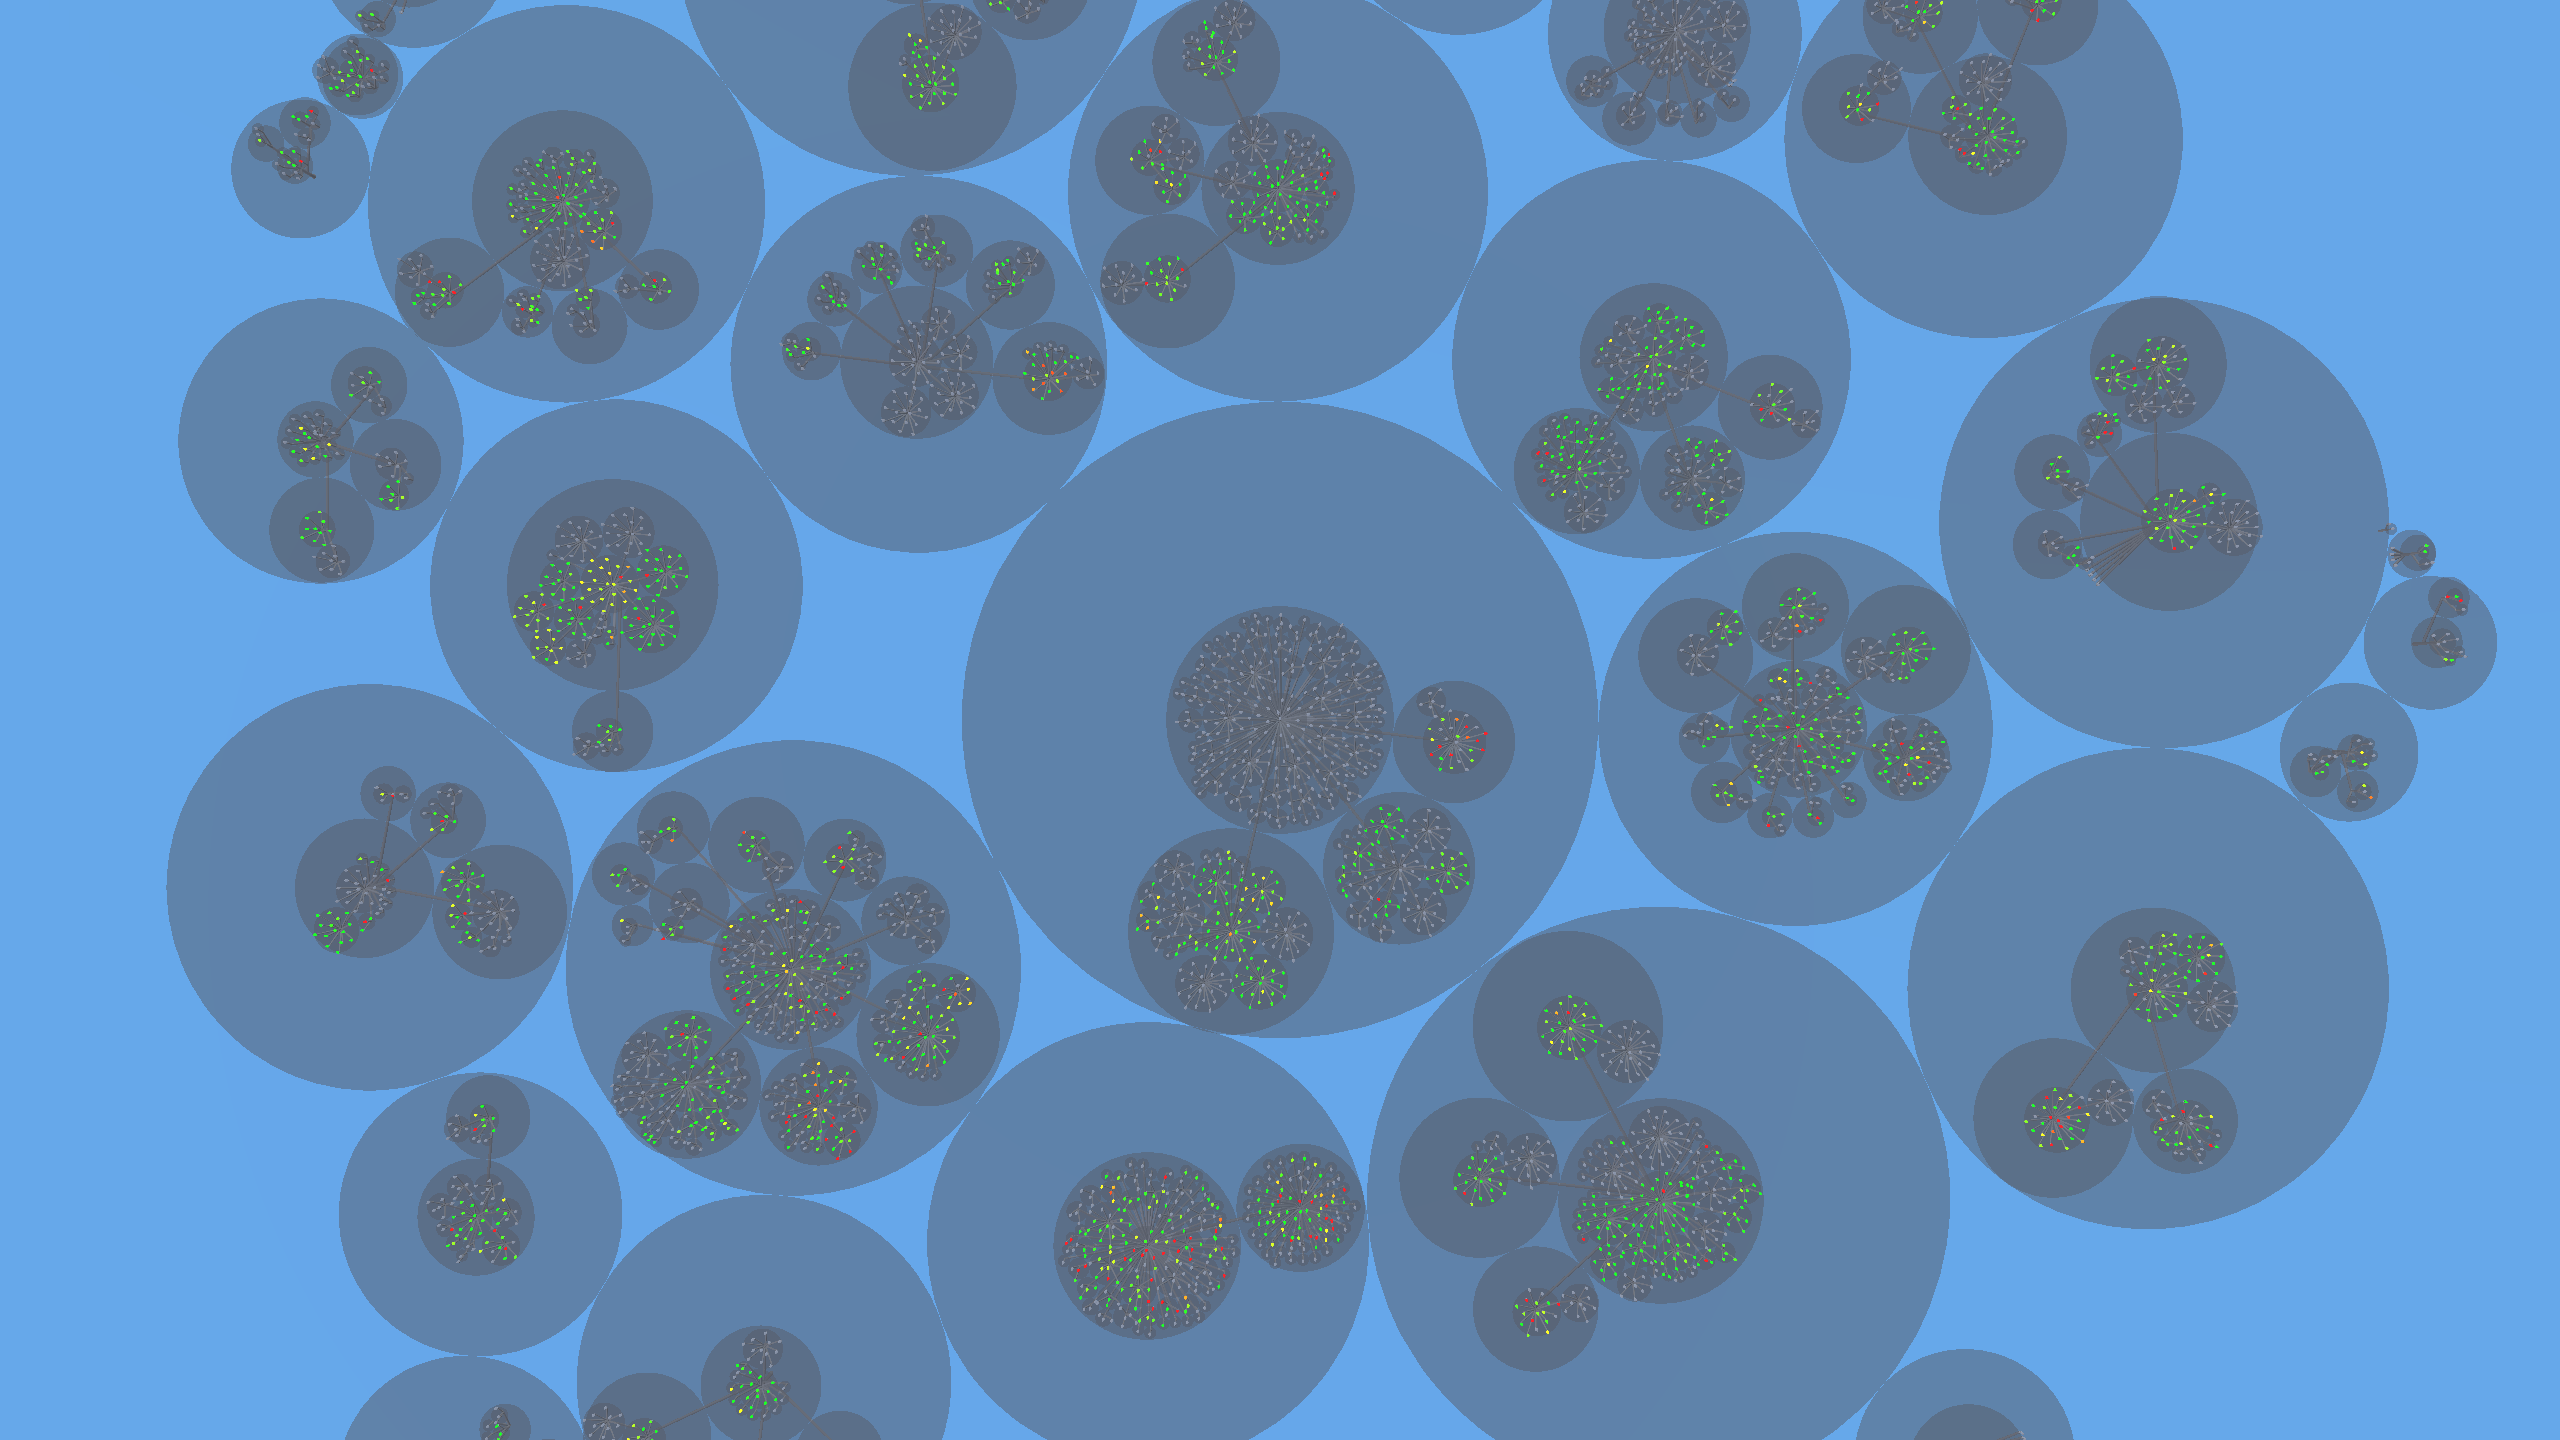
\includegraphics[width=\textwidth]{figures/circle-packing-2}
  	\subcaption{Vogelperspektive mit visualisierten Circle-Packing} \label{fig:title-bar}
  \end{subfigure}
  \caption{Layout des Waldes} \label{fig:app-menu}
\end{figure}


Auch das Circle-Packing ist durch die Kreise gut zu sehen. Jedoch lässt sich feststellen, dass durch die Wahl des größten umschließenden Kreises Platz "verschenkt" wird. Besonders in der Mitte der Abbildung wird dies durch die große Fläche deutlich, in der keine weiteren Knoten platziert sind, deutlich.

Um das zu umgehen müsste anstelle des größten umschließenden Kreises, der minimal umschließende Kreis verwendet werden. Dies ist ein weiteres mathematisches Problem und als Teil des \textit{Appollonius} Problem bekannt \cite{dergiades2007soddy}.

\todo{Vielleicht noch auf appollonius kreise eingehen}

Für den Prototyp ist die Umsetzung des kleinsten umschließenden Kreises für CodeLeaves aber nicht essentiell. Entscheidend ist, dass die Struktur der visualisierten Software ohne Überschneidungen dargestellt wird, was auch mit dem größten umschließenden Kreis möglich ist. Die Umstellung auf den kleinsten umschließenden Kreis ist deshalb eine weiterführende Aufgabe.

\section{Verwendete Algorithmen in der Praxis}

Für die Praxis in Unity ist bei der Verteilung der Bäume noch zu beachten, dass deren Radien erst verfügbar sind, nachdem der Circle-Packing-Algorithmus für alle Bäume vollständig durchlaufen wurde. Das heißt, dass bei der Generierung der einzelnen Bäume noch nicht bekannt ist, an welcher Position die Bäume letztendlich gesetzt werden müssen und zunächst zum Beispiel an der gleichen Stelle generiert werden müssen. Das bedeutet wiederum, dass bei asynchroner Programmierung und großen Projekten wie Air zunächst die Bäume überlagernd gerendert werden und dies auch durchaus für einige Sekunden für den Nutzer sichtbar ist, bevor sich die Bäume verteilen.

Bei Air dauert die Generierung der 40 Bäume im Unity Editor auf einer Hardware mit 2.3 GHz Intel Core i7 CPU und 16 GB 1600 MHz DDR3 RAM bei 10 Messungen zwischen 6,5 und 6,8 Sekunden. Auf der HoloLens stehen keine genauen Messdaten zur Verfügung, die Generierung dauert aber noch etwas länger.

Soll vermieden werden, dass der Nutzer zunächst die überlagernde Generierung mit ansieht, dürften die Bäume erst sichtbar werden, nachdem alle Bäume fertig generiert und verteilt worden sind. Jedoch ist zu beachten, dass währenddessen dem Benutzer angezeigt wird, dass der Aufbau des Waldes im Hintergrund läuft. Mehr zu diesem Thema ist im nächsten Kapitel zu finden

Ein weiterer zu beachtender Punkt ist, dass bei beschriebener Vorgehensweise einzelne Blätter theoretisch auf die gleiche Position gelangen könnten. Grund dafür ist, dass der Radius eines Knotens mit ausschließlich Blätter gleich $a_n$ gesetzt wurde. Daraus resultiert, dass bei zwei Geschwister solcher Knoten deren $n$-ten Kinder genau auf dem Schnittpunkt der Kreise liegen könnten. In diesem Fall würden sich die Blätter überschneiden. In der Praxis ist dies jedoch sehr unwahrscheinlich, besonders wenn für den Azimutwinkel des Sonnenblumen-Algorithmus ein zufälliger initialer Wert gesetzt wird, auf den dann ein Vielfaches des goldenen Winkel aufaddiert wird. In unserem Beispielprojekt mit 5373 Blättern, trat dieser Fall nicht auf.

% Current ==========================------------------------------------------------------------------------------

% ----==== Chapter ====---- %
\chapter{Grundlagen der Interaktion in der AR}
\label{ch:interaction-ar}

\section{Interaktionsmöglichkeiten der HoloLens}
\label{sec:interaction-hololens}

In den frühen 70er-Jahren wurden erste Modelle der Computermaus entwickelt und mit Apple's Lisa aus dem Jahr 1983 wurde sie zum Markterfolg. Heute ist die zeigerbasierte Interaktion mit Computer nicht mehr weg zu denken.

Neben der zeigerbasierten Eingabe hat sich mit dem Einzug von Smartphones und Tablets die touchbasierte Eingabe etabliert. Diese kann für Monitor basierte AR verwendet werden. Bei dieser Art von Mit dem AR-Kit von Apple ab der iOS Version 11 sind solche Applikationen einfach zu realisieren.

Für die AR mit Head Mounted Displays (HMD) Devices, wie es die HoloLens ist und die wie der Name schon sagt, vom Nutzer getragen werden, ergeben sich neue Möglichkeiten mit Anwendungen zu interagieren. Auch wenn z.B. die HoloLens die Eingabe durch eine Bluetooth-Maus unterstützt, bieten sich in AR zusätzliche Eingabemöglichkeiten an.

Es ergeben sich folgende Eingabemöglichkeiten für HMD-Devices:

\begin{enumerate}
  \item Blickrichtung
  \item Gesten
  \item Sprache
  \item Controller
\end{enumerate}

\subsubsection*{Blickrichtung}
Bei der HoloLens wird die Blickrichtung mit \textit{Gaze} bezeichnet und ist ein elementarer Bestandteil der Bedienung der HoloLens \cite{windows2017interaction}. Der Gaze wird im Normalfall mithilfe eines Cursers visualisiert, der der Kopfbewegung des Nutzers folgt und sich realen und virtuellen Objekten anschmiegt.

\subsubsection*{Gesten}
Nachdem bei HDM-Devices Hologramme im realen Raum platziert werden, ist Gestensteuerung eine intuitive Eingabemöglichkeit. Beispielsweise muss die Möglichkeit der Auswahl, Platzierung, Skalierung oder Rotation von Hologrammen ermöglicht werden.

Allgemein kann zischen zwei Arten von Gesten unterschieden werden.

\paragraph{Diskrete Gesten} sind solche, in denen die Ausführung der Geste einen binären Status besitzt. D.h. die Ausführung der Geste ist die Information selbst und trägt keine weiteren Informationen. Diese Gesten lassen sich mit einem Klick einer Computermaus vergleichen.

\paragraph{Kontinuierliche Gesten} sind solche, bei denen das Ausmaß der Geste eine Rolle spielt. Das Ausmaß bestimmt die Größe der Ausgabe. Vergleichen wir diese Gesten mit einer Computermaus, wäre das die Mausbewegung.\\

Theoretisch sind beliebig viele Gesten denkbar. Zum Beispiel könnte für das Rotieren von Objekten die Rotation der Hände verwendet werden. Mit Produkten wie zum Beispiel Kinetic\footnote{\url{https://developer.microsoft.com/de-de/windows/kinect}} können solche Gesten auch erkannt werden. Bei der HoloLens sind die unterstützen Gesten jedoch stark begrenzt. Es existieren insgesamt drei verschiedene Gesten, die von der HoloLens als solche identifiziert werden können. Die sogenannte \textit{Bloom}-Geste ruft das Windows Menü auf. Sie wird ausgeführt, indem der Nutzer alle Fingerspitzen zusammen führt und dann die Hand öffnet und eine aufgehende Blume imitiert.

Als weitere diskrete Geste kann der \textit{Air-tap} verwendet werden. Dieser ist in Abbildung \ref{fig:air-tap} veranschaulicht. In Verbindung mit dem Gaze können so Hologramme angeklickt werden.

\begin{figure}[htb]
  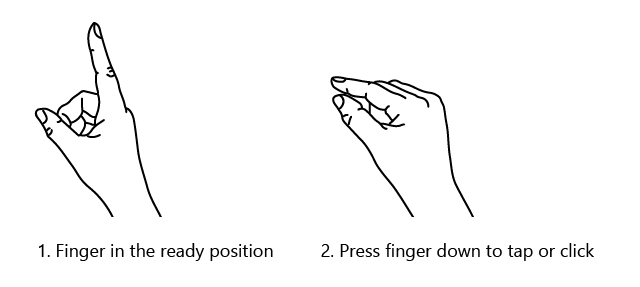
\includegraphics[width=.8\textwidth]{\figdir/air-tap}
  \caption{Air-tap \cite{windows2017gesture}}
  \label{fig:air-tap}
\end{figure}

Mit der \textit{Manipulation} Geste stellt Microsoft eine kontinuierliche Geste zur Verfügung. Wird ein Air-tap gehalten und die Hand anschließend bewegt, so kann als Ausgabe die Positionsänderung der Hand verwendet werden. Damit ist beispielsweise ein Drag and Drop von Hologrammen möglich.

Die HoloLens kann zwischen linker und rechtem Hand unterscheiden. Das bedeutet, dass auch eine Interaktion mit der Verwendung von beiden Händen möglich ist.

\subsubsection*{Sprache}
Neben den Gesten kann auch durch Sprachsteuerung mit Hologrammen interagiert werden. In einer Applikation können beliebige Sprachbefehle definiert werden, die dann von der HoloLens automatisch erkannt werden.

Da die Interaktion mit Gesten auf Dauer für die Arme ermüdend sein kann, bietet sich an, die Spracherkennung zur Unterstützung der Gestensteuerung zu verwenden. Beide Eingabemethoden können auch gut miteinander kombiniert werden. So kann z.B. mithilfe von Sprachbefehlen zwischen unterschiedlichen Interaktionsmodi umgeschalten werden. Dadurch können unterschiedliche Interaktionen wie Skalieren und Rotieren mit der gleichen Geste durchgeführt werden.

\subsubsection*{Controller}
Die vierte Möglichkeit der Interaktion mit HMD-Devices sind Controller. Die meisten VR-Headsets sind nur mit solchen Controllern zu bedienen. In der aktuellen Version unterstütz die HoloLens jedoch kein Controller. Bei anderen Windows Mixed Reality Geräten wie die \textit{Immersive} Headsets von Acer und HP\footnote{\url{https://developer.microsoft.com/en-us/windows/mixed-reality/immersive_headset_hardware_details}} kann mit den \textit{Motion} Controllern, ähnlich wie bei Gaming Konsolen, mit verschiedenen Tasten unterschiedliche Eingaben tätigen. Bei der HoloLens steht lediglich der \textit{Clicker} zur Verfügung, ein kleines Bluetooth-Gerät, dass durch physisches Klicken den Air-tap ersetzen kann. Bei Dauerhafter Eingabe von Air-tap-Gesten ist der Einsatz vom Clicker angenehm, da man die Hand nicht im Sichtfeld der HoloLens halten muss.

\section{Herausforderungen}

Bei der Entwicklung von AR-Applikationen sind einige Herausforderungen zu beachten, die auch für CodeLeaves von Relevanz sind. Im Zuge der Entwicklung von der HoloLens-Anwendung HoloStudio hat der Senior Holographic Designer Ghaly in \cite{windows2017casestudy3} eine Case Study veröffentlicht. Mitunter traten die im Folgenden betrachteten Herausforderungen auf.

\subsubsection*{Hologramme außerhalb des Sichtfelds}

Da Hologramme im ganzen Raum, in dem sich der Betrachter befindet, platziert werden können, ist nicht immer gewährleistet, dass sie sich auch im Blickfeld des Betrachters befinden. Besonders bei der aktuellen Entwickler-Version der HoloLens ist das Sichtfeld, in dem Hologramme angezeigt werden können, mit rund 30 Grad \cite{czerulla2017microsoft} gering.

Eine Variante dies zu umgehen, ist es \textit{Tag-along}-Objekte zu verwenden. Diese Objekte bleiben immer im Blickfeld des Betrachters. Schaut der Nutzer in eine andere Richtung, wird das Objekt neu positioniert, sodass es wieder im Blickfeld gelangt. Innerhalb des Blickfelds bleiben Tag-along-Objekte aber stationär, sodass der Nutzer mit dem Gaze weiterhin mit ihnen interagieren kann. Das Windows-Startmenü der HoloLens ist ein solches Tag-along-Objekt.

In der Case Study aus \cite{windows2017casestudy3} wurde festgestellt, dass die Probanden sich von solchen Tag-along-Objekten in vielen Fällen bedrängt fühlen und instinktiv versuchen davon weg zu kommen.

Eine andere Möglichkeit ist es die Hologramme stationär im Raum zu platzieren und die Aufmerksamkeit des Nutzers gezielt zu lenken. Das kann mit verschiedenen Techniken erreicht werden. Eine davon ist die Verwendung von \textit{Spacial Sound}, was bedeutet, dass Geräusche ebenfalls im Raum platziert werden können und vom Nutzer dreidimensional mit Richtung und Entfernung warngenommen werden können. Dies bietet sich vor allem bei Spielen mit bewegten Charakteren an. Bei statischem Content wie CodeLeaves, sind Geräusche nicht besonders intuitiv.

Es kann auch mit zusätzlichen Objekten gearbeitet werden, die dem Nutzer darauf hinweisen, wo sich etwas befindet, was seine Aufmerksamkeit erfordert. Solche Hilfs-Objekte nennen wir \textit{Direction Indicators}. Diese können unterschiedliche Gestalt annehmen. Bei anderen HoloLens-Applikationen sind Pfeile, Licht oder Denkblasen im Einsatz.

\subsubsection*{UI von anderen Objekten verdeckt}

Ein Problem, das in vielen HoloLens-Applikationen auftritt, ist dass UI Elemente von anderen Hologrammen, die näher am Nutzer positioniert sind, verdeckt werden können.

Das Problem ist in Abbildung \ref{fig:occlusion} illustriert. Darin wird in CodeLeaves das Menu zu Interaktion mit dem Wald der "`Move"'-Button von einem Stamm verdeckt.

\begin{figure}[htb]
  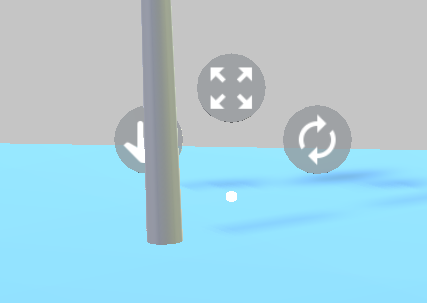
\includegraphics[width=.6\textwidth]{\figdir/occlusion}
  \caption{Verdeckung eines Buttons}
  \label{fig:occlusion}
\end{figure}

Analog zum 2D Popups ist es natürlich möglich UI Elemente vor allen anderen Elementen zu platzieren. In 3D bedeutet das, dass das UI Element vor dem Hologramm erscheinen muss, dass sich am nächsten am Nutzer befindet. Die UI Elemente würde dadurch vom eigentlichen interagierten Objekt losgelöst werden, was eine wenig intuitive Interaktion darstellt. Dies kann aber zu Folge haben, dass der Nutzer irritiert wird, weil er mit etwas weiter weg interagiert und die UI deutlich weiter vorne erscheinen kann.

Eine Abhilfe kann ein \textit{Shine-through}-Effekt schaffen, wie er bei HoloStudio Verwendung findet. Dabei bleiben UI Elemente an dem Hologramm angeheftet, mit dem interagiert wird, jedoch scheinen sie durch davor liegende Hologramme durch.

\begin{figure}[htb]
  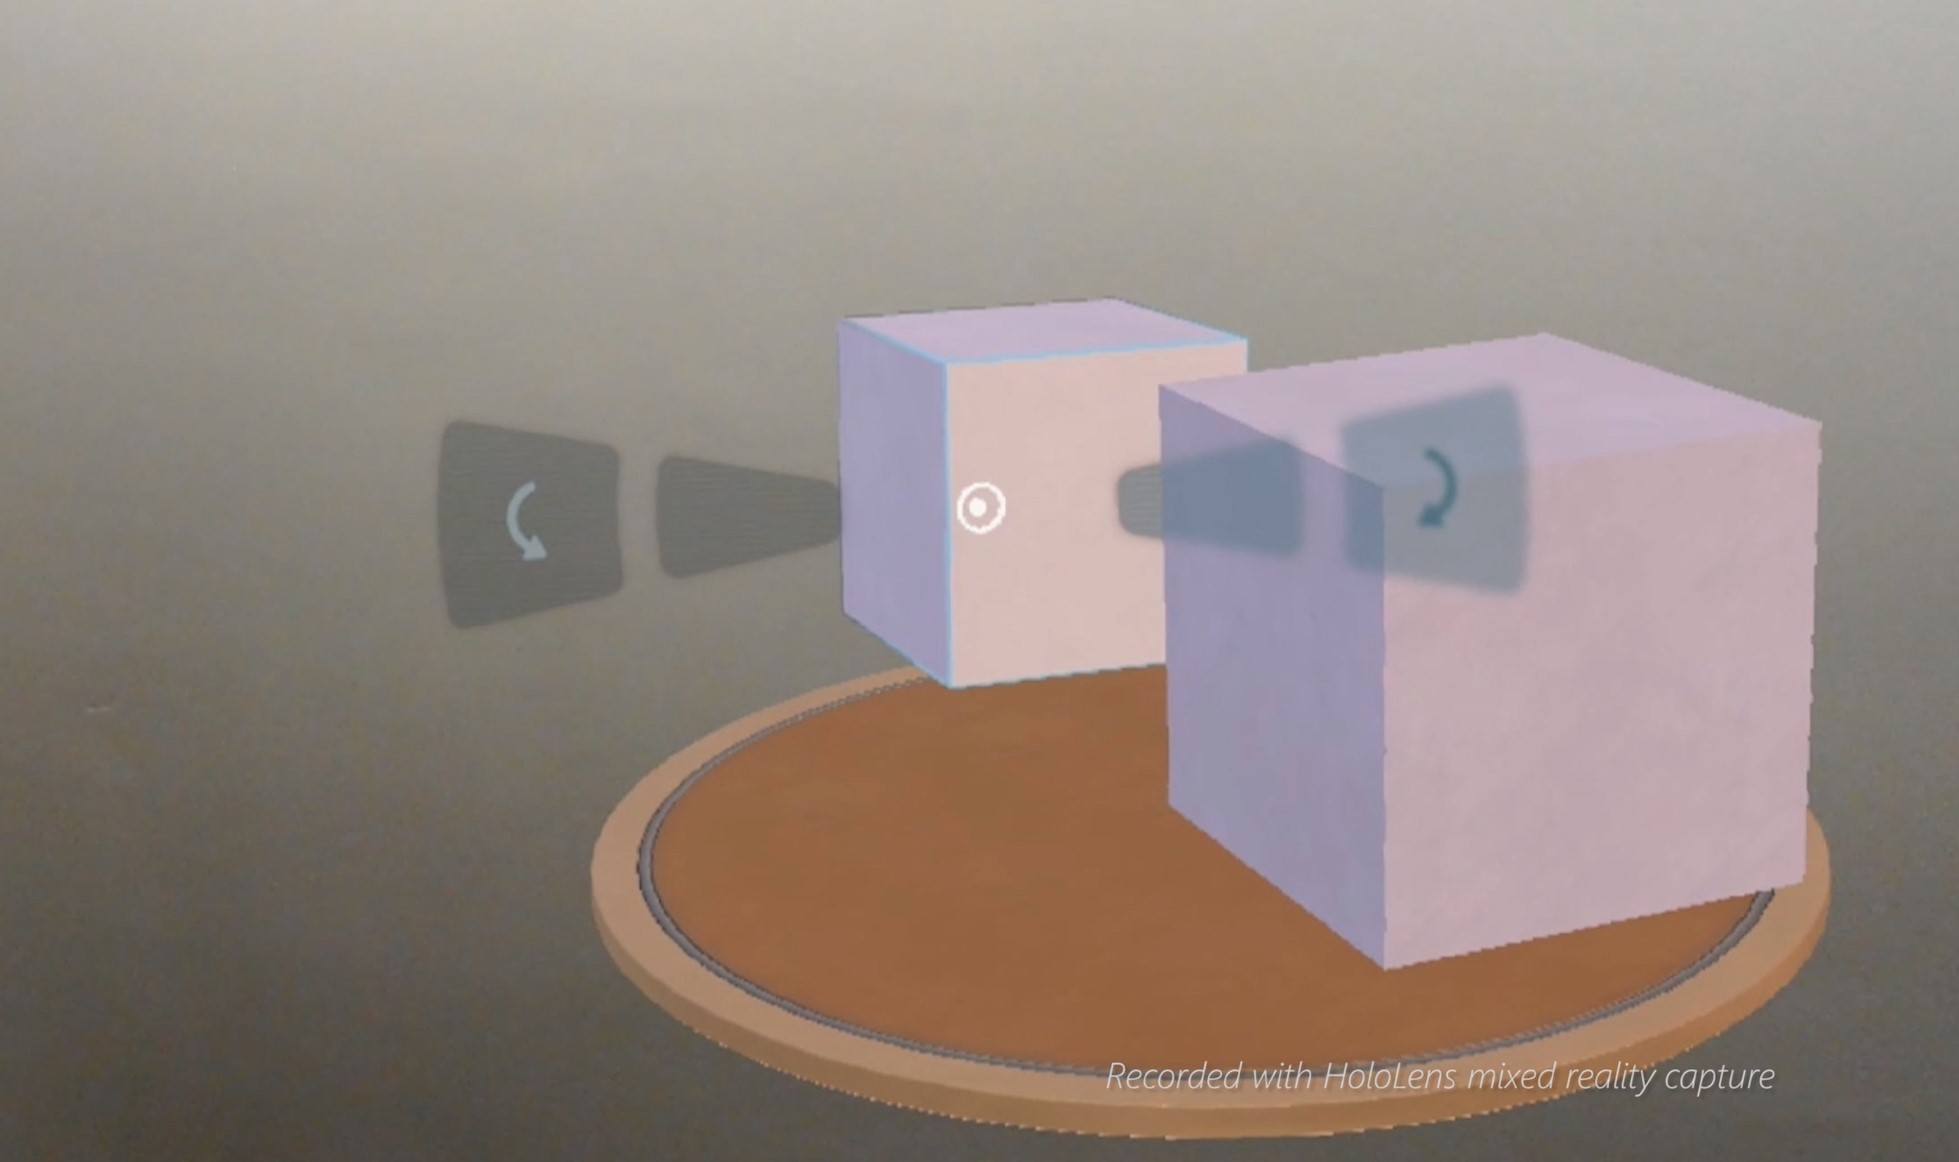
\includegraphics[width=.6\textwidth]{\figdir/shine-through}
  \caption{Shine-through-Effect von UI Elementen in HoloStudio \cite{windows2017casestudy3}}
  \label{fig:shine-through}
\end{figure}

Diese Methode funktioniert jedoch schlecht, wenn die UI Elemente Texte sind und von davor liegenden Texten verdeckt werden. Dadurch werden beide Texte unleserlich. Dieses Problem tritt z.B. zwangsläufig bei der Beschriftung von Blättern in CodeLeaves auf und lässt sich nur vermeiden, indem einer der beiden Texte verschwindet oder zumindest verblasst.

Die betrachteten Herausforderungen von 3D Interaktion und deren mögliche Lösungsansätze finden sich im Interaktionskonzept von CodeLeaves wieder und werden in Abschnitt \ref{sec:interaction} aufgegriffen.

\section{Technische Umsetzung von Interaktionen mit Reaktiver UI}

\subsubsection*{Motivation}
Eine der offensichtlichen Interaktionen mit CodeLeaves ist das Anklicken von Knoten, seien es Blätter oder die dazugehörigen Kanten. Der Nutzer erwartet damit nähere Informationen zu einem Paket oder einer Klasse zu erfahren. Betrachten wir zunächst eine sehr einfaches Szenario:

\begin{quotation}
  \textit{Wenn der Nutzer auf ein Blatt klickt, soll daraufhin der Name der repräsentierten Klasse über dem Blatt erscheinen.}
\end{quotation}

Diese Interaktion ist in Abbildung \ref{fig:leaf-interaction} veranschaulicht.

\setlength{\fwidth}{.49\textwidth}
\begin{figure}[htb]
  \centering
  \begin{subfigure}[b]{\fwidth}
   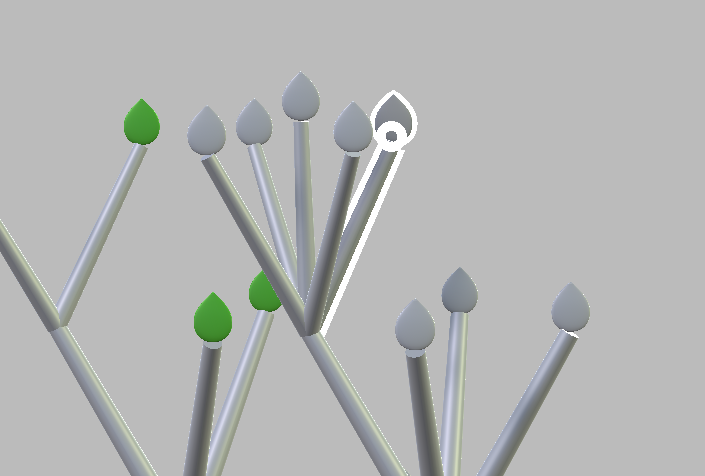
\includegraphics[width=\textwidth]{figures/leaf-focused}
   \subcaption{Fokussiertes Blatt} \label{fig:leaf-focused}
  \end{subfigure}
  \hfill
  \begin{subfigure}[b]{\fwidth}
  	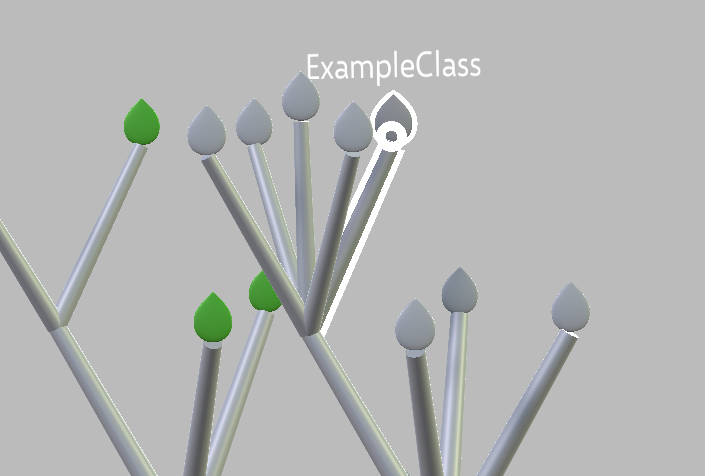
\includegraphics[width=\textwidth]{figures/leaf-clicked}
  	\subcaption{Angeklicktes Blatt} \label{fig:leaf-clicked}
  \end{subfigure}
  \caption{Anzeige des Klassennamens durch Klick auf ein Blatt} \label{fig:leaf-interaction}
\end{figure}

Bei der Generierung des Baumes wird zu jedem Blatt ein Label hinzugefügt, in dem der Klassenname gespeichert werden kann. Das Anzeigen Namens ist demnach kein Problem und würde wie folgt funktionieren:

\begin{codesnippet}{Direkte Manipulation (Negativbeispiel)}{lst:direct-manipulation}
public class NodeInputHandler : MonoBehaviour, IInputClickHandler
{
    public void OnInputClicked(InputClickedEventData eventData)
    {
        // Get label of currently clicked node
        var labelObject = GetLabelObject(gameObject);

        // Toggle active
        labelObject.SetActive(!labelObject.activeSelf);
    }
}
\end{codesnippet}

Im traditionellen Ansatz könnte also auf das Ereignis des Air-taps auf einfachste Weise reagiert werden. Wird das Blatt angeklickt, wird das Label-Objekt des Blattes aktiviert und der Name wird damit sichtbar. Entsprechend kann bei erneutem Klick das Label-Objekt wieder deaktiviert werden. Wird die Businesslogik aber komplexer, kommt dieser Ansatz schnell an seine Grenzen.

Eventuell könnte sich zum Beispiel folgende Einstellung in der Applikation als sinnvoll erweisen:

\begin{quotation}
  \textit{Der Nutzer kann einstellen, ob bei einem Klick auf ein Blatt der Klassenname oder die Zahl der gerade visualisierten Metrik angezeigt wird.}
\end{quotation}

Woher weiß die Funktion jetzt was angezeigt werden soll?

Das eigentliche Problem bei der beschriebenen Situation ist, dass Businesslogik und UI eng gekoppelt wurde. Dies sollte tunlichst vermieden werden. Bei einem Klick auf einem Blatt sollte nicht die UI entscheiden was zu tun ist, sondern die Businesslogik. Die Entkopplung von UI und Logik, ist mit reaktiver Programmierung möglich.

Was ist reaktive Programmierung? Staltz beschreibt es in \cite{staltz2016introduction} als "`Programmierung mit asynchronen Datenströmen."' Dies trifft den Kern. Es geht darum auf Änderungen von Werten zu reagieren, die durch \textit{Streams} propagiert werden.

Streams sind nichts anderes als \textit{Observables} die bei jeder Änderung ihrer Werte allen registrierten \textit{Subscribers} den neuen Wert mitteilen.

Betrachten wir in Abbildung \ref{fig:label-stream} konkret das Beispiel den Text, der im Label eines Blattes steht.

\begin{figure}[htb]
  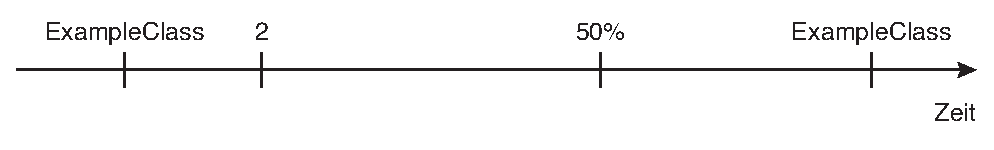
\includegraphics[width=.8\textwidth]{\figdir/label-stream}
  \caption{Datenstrom des Labels}
  \label{fig:label-stream}
\end{figure}

Über die Zeit hinweg, kann sich durch die Businesslogik der darzustellende Text verändern. Im Beispiel soll der Klassenname, dann vielleicht Laufzeitfehler, Coverage und dann wieder der Klassenname dargestellt werden.

Bei der Generierung des Baumes muss dann lediglich der Label-Wert observiert und der Text entsprechend gesetzt werden.

\subsubsection*{Verwendung in Unity}

In Unity steht für reaktive Programmierung das Open-Source-Projekt \textit{UniRx}\footnote{\url{https://github.com/neuecc/UniRx}} zur Verfügung, das die Funktionalität der reaktiven .NET Library \textit{Rx} für Unity zugänglich macht. UniRx implementiert z.B. \textit{ReactiveProperties}, mit denen eine einfache Verwendung des Observer-Pattern möglich ist. Darüber hinaus bietet die API hilfreiche Stream-Funktionen wie filter, map, merge oder join.

In unserem Beispiel von oben wird der Text eines Blattes des UI-Models zu einer ReactiveProperty und bei jeder Änderung wird der Text des Labels angepasst. Auch das aktivieren des Labels wird über eine ReactiveProperty realisiert. So ist zum Beispiel das deaktivieren von allen Labels gleichzeitig leicht möglich.

In Listing \ref{lst:reactive-property} wird gezeigt, wie eine ReactiveProperty für den Status \texttt{isSelected} eines UI-Knotens definiert wird. Im \texttt{TreeBuilder} (Zeile 9) wird das Label bei Aktualisierung von \texttt{isSelected} entsprechend aktiviert.

\begin{codesnippet}{Observieren von Werten}{lst:reactive-property}
public abstract class UiNode
{
    public ReactiveProperty<bool> isSelected { get; set; }
    ...
}

public class TreeBuilder {
    ...
    node.IsSelected.Subscribe(label.SetActive);
    ...
}

public class NodeInputHandler : MonoBehaviour, IInputClickHandler
{
    public void OnInputClicked(InputClickedEventData eventData)
    {
        Store.Dispatch(NodeClickAction(GetNodeId(gameObject)));
    }
    ...
}
\end{codesnippet}

Im \textit{NodeInputHandler} wird nun nicht mehr direkt auf die UI zugegriffen, sondern es wird ein Funktion aufgerufen, die sich darum kümmert, dass das UI-Model editiert. Hier kommt zusätzlich Redux\footnote{\url{http://redux.js.org/}} ins Spiel.

\subsubsection*{Redux}
Mit UniRx kann auf Änderung eines Models in der UI reagiert werden. Redux ist ein Konzept, das noch ein Schritt weiter geht. Die Grundidee ist, dass der komplette Status einer App in einem \textit{State} gespeichert wird. Der State kann durch \textit{Reducer}, reinen Funktionen transformiert werden. Diese wiederum haben als Input wohl definierte \textit{Actions}, welche durch Interaktion mit der UI \textit{dispatched} werden. Der State, die Reducer und die Möglichkeit Actions zu versenden sind Inhalt des \textit{Stores} \cite{abramov2017redux}.

Diesem Prinzip folgenden ist auch die Interaktion von CodeLeaves aufgebaut. Dadurch wird einen nachvollziehbaren Datenfluss garantiert und eine technische Basis für ein Interaktionskonzept geschaffen.

\chapter{Interaktion mit CodeLeaves}
\label{sec:interaction}

CodeLeaves kann ohne Interaktion die Struktur einer Software, eine Metrik und Verbindungen zwischen Softwareartefakten darstellen. Damit kann bereits einen Überblick über die Software geschaffen werden. Der wirklichen Mehrwert von CodeLeaves wird aber erst erreicht, wenn mit dem Software-Wald interagiert wird. Die intuitive Bedienung von CodeLeaves ist demnach essentiell für eine gute User Experience und damit ein tieferes Verständnis der visualisierten Informationen.

\section{Basisinteraktionen}
Grundlegend muss der gesamte Wald einige \textit{Basisinteraktionen} unterstützen. Diese sind:

\begin{itemize}
  \item Platzieren
  \item Skalieren
  \item Rotieren
\end{itemize}

Das Platzieren ist von Anfang an notwendig um den Wald im Raum dahin zu setzten, wo es für den Nutzer am meisten Sinn macht. Bequemerweise kann das z.B. auf einem Tisch sein, oder wenn ein solcher nicht zur Verfügung steht auch auf dem Fußboden. Wenig hilfreich wäre es aber wenn er über dem Benutzer schwebt.

Das Skalieren ist auch unterlässlich. Gerade bei großen Systemen kann auch der Wald sehr groß werden. Daher muss die Größe des Waldes auf die Gegebenheiten der Räumlichkeiten angepasst werden können.

Ist der Wald einmal platziert und skaliert, möchte der Nutzer sich den Wald von allen Seiten anschauen können. Er kann natürlich darum herumlaufen, aber vielleicht reicht der Platz dazu nicht aus, oder ein Drehen des Waldes selbst ist bequemer.

\subsubsection*{Bounding Box}

Das Repository "`Mixed Reality Design Labs"' bietet für genau diese Interaktionen eine Lösung. Die \textit{Bounding Box}, wie sie in Abbildung \ref{fig:bounding-box} zu sehen ist, rendert ein 3D Rahmen um das zu manipulierende Objekt. Das Platzieren des Objekts kann mit einer Manipulation auf den gesamten Bereich der Bounding Box erreicht werden. Mit den kleinen Würfeln an den Ecken der Bounding Box kann skaliert werden und die kleine Kugeln auf den vertikalen Kanten der Bounding Box ist für das Rotieren vorgesehen.

\begin{figure}[htb]
  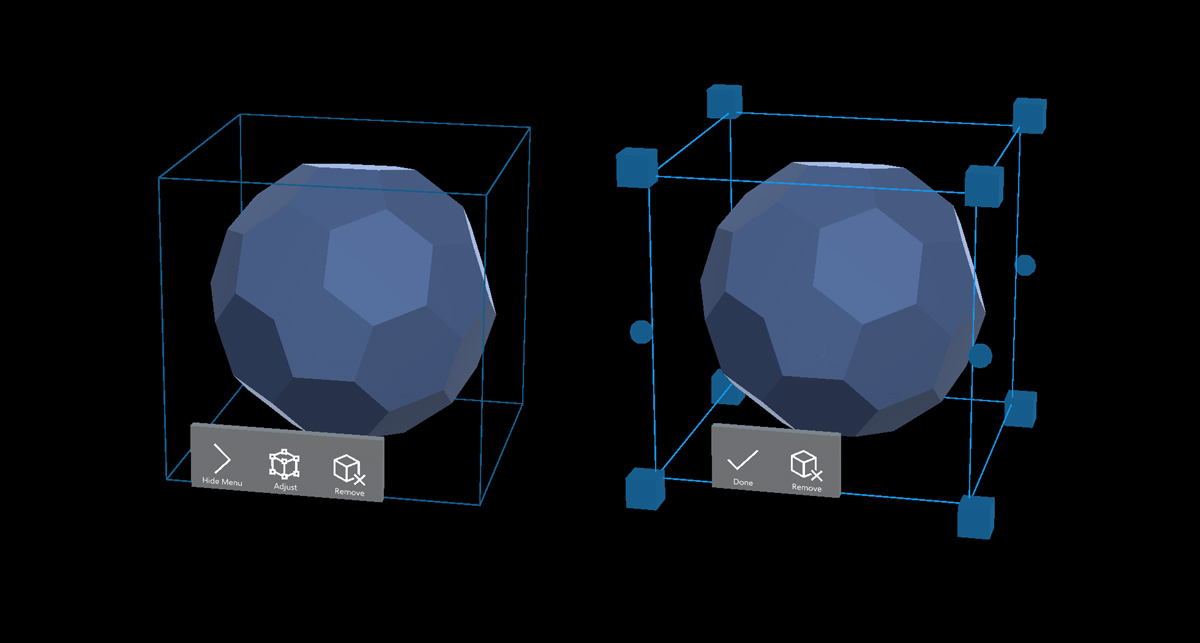
\includegraphics[width=.8\textwidth]{\figdir/bounding-box}
  \caption{Bounding Box zum Platzieren, Skalieren und Rotieren von Objekten \cite{microsoft2017mixed}}
  \label{fig:bounding-box}
\end{figure}

Dieser Ansatz hat den Vorteil, dass dem Nutzer ein Interface angeboten wird, das ihm aus dem Zweidimensionalen wohl bekannt ist. In den meisten Applikationen mitunter in den Bereichen Text- und Bild- oder Grafikverarbeitung ist die Bounding Box Standard. In die Dreidimensionalität übertragen kennt der Nutzer das Prinzip und weiß was er für eine gewünschtes Ziel zu tun hat.

\subsubsection*{Interaktionsmodi}

Für CodeLeaves ist dieser Ansatz jedoch aus einem einfachen Grund schwierig. Der Wald muss nicht zwangsläufig in seiner Gänze im Blickfeld des Nutzers sein. Angenommen der Nutzer interessiert sich vor allem für ein bestimmten Baum, möchte er diesen genauer betrachten und vergrößert den Wald soweit, dass andere Bäume aus dem Sichtfeld verschwinden. Möchte er dann den Wald wieder verkleinern, müsste er erst soweit zurück gehen, bis er die Bounding Box nutzen kann. Das ist aber aufgrund der Räumlichkeiten vielleicht gar nicht möglich und wenn doch nicht besonders benutzerfreundlich.

Eine Alternative muss daher gefunden werden. Es stellt sich die Frage, was immer im Sichtfeld des Nutzers ist und den Wald für den Nutzer als Ganzes repräsentiert. Der Waldboden als Antwort auf diese Frage leuchtet ein. Er ist auch bei näherer Betrachtung einzelner Teile von CodeLeaves immer präsent und da alles aus ihm wächst ist eine Interaktion mit ihm für die Basisinteraktionen intuitiv.

Damit steht das Ziel der Interaktion fest, jedoch können mit der begrenzten Anzahl an Gesten nicht alle Basisinteraktionen mit dem gleichen Ziel bedient werden. Daher wird bei einem Air-tap ein Kontextmenü dargestellt, mit dem der Nutzer zwischen den drei verschiedenen Basisinteraktionen wählen kann. Bei der Auswahl der Modi Skalieren und Rotieren kann der Nutzer mithilfe der Manipulation-Geste und fokussiertem Waldboden den Wald entsprechend manipulieren. Die Ausführung dieser Geste werden näher im Abschnitt \ref{subsec:manipulation-indicators} ausgeführt.

\subsubsection*{Interaktion mit Spacial Mapping}
Für den Plazierungs-Modus bietet sich für die HoloLens die Nutzung des \textit{Spacial Mapping} an. Die HoloLens ist fähig den Raum, in dem sie sich befindet, zur Laufzeit zu erfassen und einer Applikation zur Verfügung zu stellen \cite{windows2017spacial}. Mit diesen Informationen ist es Möglich ein Spatial Mapping Mesh darzustellen, das über die reale Oberfläche des Raumes gelegt wird. Damit können Hologramme mit der Oberfläche des Raumes kollidieren und entsprechend der Umgebung platziert werden. So ist es zum Beispiel möglich den Wald auf einen Tisch oder auf den Boden zu positionieren.

Bei aktivem Platzieren des Waldes wird des Spatial Mapping Mesh angezeigt, sodass der Nutzer sieht, wo genau der Waldboden mit der Umgebung kollidiert. Die Positionierung selbst wird nicht mit der Manipulation-Geste ausgeführt, sondern mithilfe des Gaze. Der Wald folgt der Blickrichtung des Nutzers und wird immer dort platziert, wo die Blickrichtung das Spatial Mapping Mesh trifft. Die Manipulation-Geste ist besonders für die Eingabe eines Deltas geeignet. Für den Input einer bestimmten Richtung, die für Kollision mit dem Spatial Mapping Mesh benötigt wird, ist der Gaze die bessere Wahl. Zudem ist der "`Transport"' des Waldes auf diese Weise auch über größere Strecken komfortabel, da die Hand des Nutzers nicht dauerhaft oben gehalten werden muss, wie es bei der Manipulation nötig wäre. 

Der Modus des Platzieren wird durch einen Air-tap auf den Wald beendet. Der aktive Modus mit dem Spatial Mapping Mesh kann in Abbildung \ref{fig:spatial-mapping} betrachtet werden.

\begin{figure}[htb]
  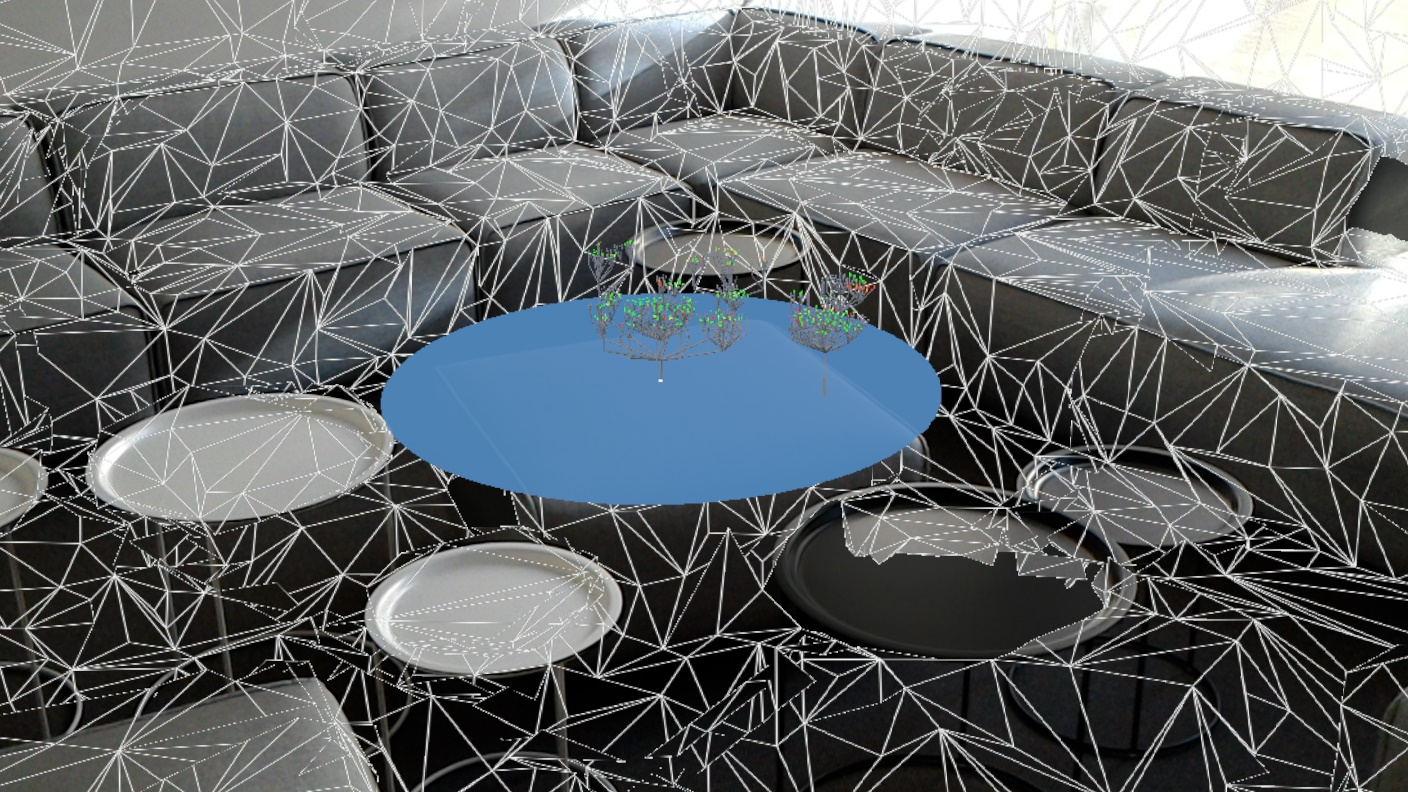
\includegraphics[width=.8\textwidth]{\figdir/spatial-mapping}
  \caption{Spacial Mapping beim Platzieren des Waldes}
  \label{fig:spatial-mapping}
\end{figure}

\section{Das Kontextmenü}
Das Kontextmenü, mit dem die verschiedenen Interaktionsmodi für den gesamten Wald ausgewählt werden können, lässt sich aber nicht nur für die Interaktion mit dem Waldboden anwenden. Auch für andere fokussierte Objekte ist eine vom Kontext abhängige Auswahl von möglichen Funktionen allgemeingültig sinnvoll. In herkömmlichen 2D User Interfaces ist dies mit einem Rechtsklick zu vergleichen. In 3D kann um den Punkt, den der Nutzer beim Aufruf des Kontextmenüs fokussiert hatte, das Kontextmenü als Buttons in einer kreissegmentförmigen Anordnung dargestellt werden.

Die kreissegmentförmige Anordnung der Buttons hat den Vorteil, dass der Interaktionspunkt für das öffnen des Kontextmenüs im Zentrum des Kreises ist und daher eine Verbindung mit dem fokussieren Objekt schafft. Darüber hinaus sind alle Buttons vom Cursor gleich weit entfernt und daher schnellstmöglich mithilfe des Gaze erreichbar.

Die Distanz des Kontextmenüs ist den Umständen entsprechend anzupassen. Ist der fokussierte Punkt bereits näher als die Distanz, in der eine Darstellung von Interaktionselementen empfohlen wird\footnote{Die Distanz, in der es empfohlen ist Hologramme zu platzieren, liegt bei 2,0 Metern \cite{windows2017interaction}}, sollte das Kontextmenü nicht noch näher an dem Nutzer platziert werden. Bei größerem Abstand sollte der Abstand zum Kontextmenü auf die empfohlene Distanz reduziert werden, sodass der Nutzer noch komfortabel mit dem Menü interagieren kann.

In dem Fall, dass das Kontextmenü direkt an der fokussierten Position erscheint, muss das Kreissegment des Kontextmenüs so angepasst werden, dass die Buttons nicht in das fokussierte Objekt hinein ragen. Für den Waldboden ist daher ein nach oben orientiertes Kreissegment eine gute Wahl. Würde aber zum Beispiel mit einer Wand interagiert werden, sollte das Kontextmenü von der Wand weg orientiert sein.

Das Kontextmenü für den Waldboden im Prototypen ist in Abbildung \ref{fig:context-menu} zu sehen. Mit dem vierten Button von links ist das App-Menü aufrufbar, dass in \ref{subsec:app-menu} vorgestellt wird. 

\begin{figure}[htb]
  \centering
  \begin{subfigure}[b]{\fwidth}
    \centering
    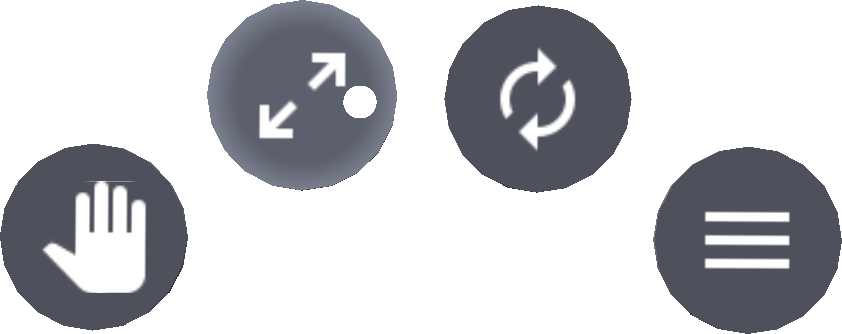
\includegraphics[height=2.5cm]{figures/context-menu-front}
    \subcaption{Kontextmenü aus Sicht des Nutzers} \label{fig:context-menu-front}
  \end{subfigure}
  \begin{subfigure}[b]{\fwidth}
    \centering
  	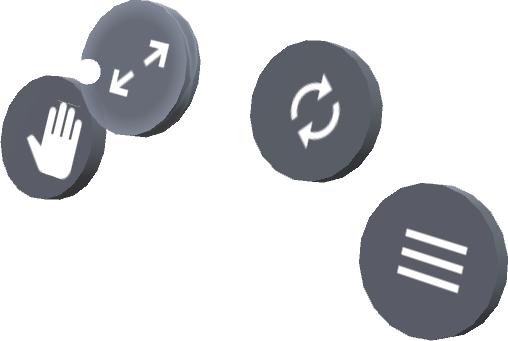
\includegraphics[height=2.5cm]{figures/context-menu-side}
  	\subcaption{Kontextmenü von der Seite} \label{fig:context-menu-side}
  \end{subfigure}
  \caption{Kontextmenü des Waldbodens im HoloLens Prototyp} \label{fig:context-menu}
\end{figure}

In Abbildung \ref{fig:context-menu-side} ist zu erkennen, dass der fokussierte Button räumlich hervorgehoben ist. Dies ist eine vor der Augmented Reality noch nicht dagewesene Möglichkeit dem Nutzer Feedback zu geben. Angenommen $\vv{g}$ ist der Normalvektor des Gaze des Nutzers, dann wird ein Button beim Fokussieren um $-\vv{g} \cdot x$ transformiert, wobei $x$ ein beliebiger Faktor ist. Bei der Ausführung der Air-tap-Geste wird beim Schließen der Finger der Button um $\vv{g} \cdot x$ transformiert, sodass er wieder in seine Ausgangsposition gelangt. Sobald der Nutzer mit dem Öffnen der Finger den Air-tap beendet, wird der Button wieder um $-\vv{g} \cdot x$ transformiert. Verlässt der Fokus den Button, wird er ebenfalls wieder in seine Ausgangsposition versetzt.

Mit diesem Prinzip wird einem Button ein haptisches Feedback verliehen und der Nutzer kann ihn räumlich "`eindrücken"'. Das Prinzip findet auch beim Windows-Menü der HoloLens Anwendung und zieht sich durch die gesamte UI des Prototypen.

\section{Manipulation-indicators}
\label{subsec:manipulation-indicators}
Mit dem Kontext-Menü des Waldbodens kann zwischen den beiden Interaktionsmodi umgeschalten werden, die mit der Manipulation-Geste ausgeführt werden. Bei der Manipulation-Geste weiß der Nutzer aber ohne weiter Hilfe nicht, wie er seine Hand bewegen muss, um die gewünschte Manipulation zu erreichen. Möchte der Nutzer beispielsweise den Wald verkleinern, weiß er nicht in welche Richtung der Wald vergrößert wird und in welche verkleinert. Zudem sind mehrere Bewegungsachsen wie horizontal, vertikal oder diagonal denkbar. Deswegen ist es unerlässlich dem Nutzer Feedback zu geben. Dies wird mit den -- wie wir sie nennen -- \textit{Manipulation-indicators} erreicht. Diese tauchen auf, sobald der Air-tap gehalten wird und indizieren die möglichen Richtungen und deren Auswirkung.

In Abbildung \ref{fig:manipulation} sind Manipulation-indicators für das Beispiel des Skalieren dargestellt.

\begin{figure}[htb]
  \centering
  \begin{subfigure}[t]{\fwidth}
    \centering
    
\includegraphics[height=1.5cm]{figures/manipulation}
    \subcaption{Initialer Zustand} \label{fig:manipulation}
  \end{subfigure}
  \begin{subfigure}[t]{\fwidth}
    \centering
  	
\includegraphics[height=1.5cm]{figures/manipulation-drag}
  	\subcaption{Darstellung des Deltas durch Bewegung der Pfeile} \label{fig:manipulation-drag}
  \end{subfigure}
  \caption{Manipulation-indicators am Beispiel des Interaktions-Modus Skalieren} \label{fig:manipulation}
\end{figure}

Durch die Pfeile wird die Achse der Manipulation angegeben. In unserem Beispiel wird die Horizontale für die Skalierung verwendet. Durch die Symbole wird dem Nutzer eindeutig angezeigt, welche Richtung welche Auswirkung hat. Durch die Verschiebung der Pfeile um das Delta der Handposition, wird dem Nutzer zudem das Ausmaß seiner Eingabe widergespiegelt.

\section{Das App-Menü}

Bisher wurden Interaktionen behandelt, die nur bei einem vorhanden Wald relevant sind. Der Nutzer von CodeLeaves muss jedoch zuvor auswählen können, welche Software er überhaupt visualisieren möchte. Auch müssen die dargestellten Informationen nach der Auswahl eines Projekts konfiguriert werden können. Dafür wird ein zentrales \textit{App-Menü} eingeführt.

Für dieses Menü wurde sich an herkömmlichen Fenstern orientiert, wie sie bei Desktop-Systemen zu finden sind. Bevor näher auf den Inhalt des App-Menüs eingegangen wird, muss zunächst auf die Positionierung des Fensters im Raum eingegangen werden.

\subsubsection*{Positionierung}

Initial dient das App-Menü dazu ein Projekt auszuwählen bzw. eines von einer unterstützen Datenquelle auszuwählen. Deshalb sollte das Menü nach dem Start der App in jedem Fall im Fokus des Nutzers platzieret werden, sodass der Nutzer sofort mit CodeLeaves arbeiten kann. Dies kann mit dem in Abschnitt \ref{sec:interaction-hololens} vorgestellten Tag-along-Effekt bewerkstelligt werden. Für den initialen Zustand ist der Tag-along-Effekt des App-Menüs als nicht störend zu bewerten, da der Nutzer in jedem Fall mit dem Menü interagieren möchte und noch keine andren Inhalte vorhanden sind, die das Menü verdecken würde.

Nach der Auswahl eines Projekts muss der Tag-along-Effekt aber als störend empfunden werden, da er das Menü im Vordergrund hält und die Sicht auf den Wald versperrt. Das Fenster des App-Menüs muss demnach die Möglichkeit unterstützen stationär im Raum platziert zu werden oder ganz geschlossen zu werden.

Zweiteres kann mit einem Schließen-Button in einer Titelleiste realisiert werden, was dem Nutzer aus bekannten Systemen vertraut ist. Das erneute Öffnen kann und muss durch das Kontextmenü möglich sein. In Abbildung \ref{fig:context-menu} ist diese Möglichkeit im Kontextmenü des Waldbodens bereits zu sehen gewesen. Auch im Kontextmenü eines Blattes oder eines inneren Knotens sollte das App-Menü aufrufbar sein, da der Nutzer damit Eigenschaften der Blätter und inneren Knoten verändern kann.

Die Funktion des stationären Platzierens kann ebenfalls in der Titelleiste untergebracht werden. Analog zum "`Vollbild"' eines Desktop-Fensters, bei dem der Nutzer sich ausschließlich auf dieses konzentrieren möchte, wird neben dem Schließen-Button ein neuer \textit{Tag-along-Button} eingeführt, der für das Ein- und Ausschalten des Tag-along-Effekts zuständig ist. Damit kann der Nutzer das Fenster jederzeit dort platzieren, wo es sich gerade befindet. Wurde das App-Menü zuvor geschlossen, wird beim erneuten Öffnen des Fensters durch das Kontextmenü der Tag-along-Effekt aktiviert, sodass der Nutzer das Fenster nicht suchen muss, sondern zu ihm kommt, sobald er es braucht.

Die Titelleiste kann für eine weitere Funktion genutzt werden. Wird bei Desktop-Sytemen ein Drag-and-drop der Titelleiste durchgeführt, lässt das zugehörige Fenster verschieben. Dies ist in 3D ebenfalls möglich. Wird die Manipulation-Geste bei fokussierter Titelleiste durchgeführt, wird das Fenster des App-Menüs entsprechen im Raum verschoben. Durch die dreidimensionale Eingabe der Manipulation und Faktor, kann der Drag-and-drop im Zweidimensionalen einfach in drei Dimensionen übertragen werden.

In dem HoloLens Prototyp wurden die beschriebenen Funktionen des App-Menüs bereits umgesetzt. In Abbildung \ref{fig:app-menu} kann das erstellte Menü betrachtet werden. Die Auswahl eines Projekts beschränkt sich dabei auf Beispielprojekte.

\begin{figure}[htb]
  \centering
  \begin{subfigure}[t]{\textwidth}
    \centering
    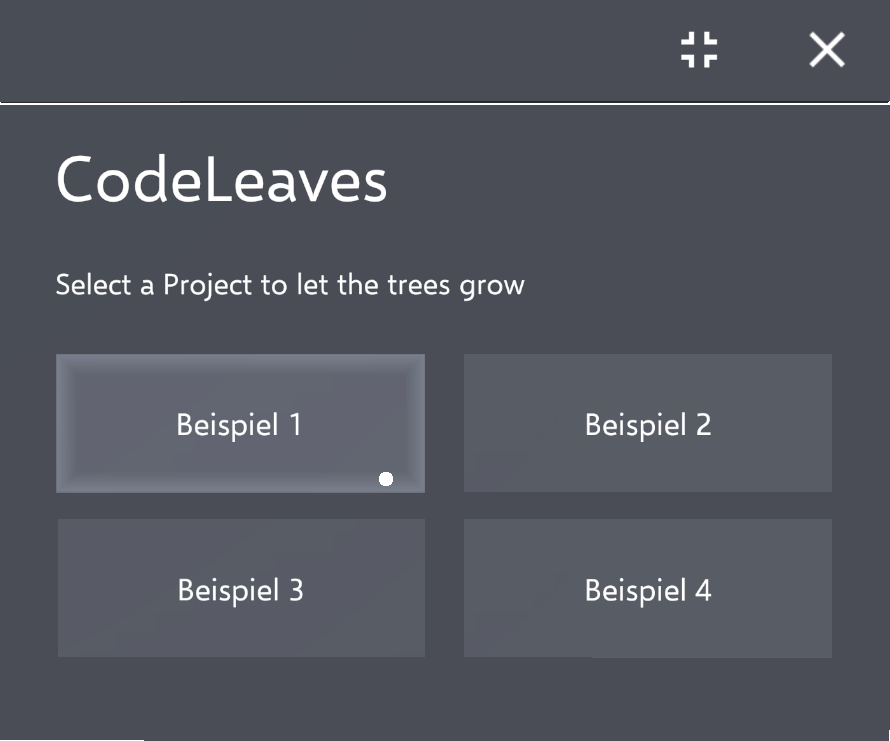
\includegraphics[width=.8\textwidth]{figures/project-selection}
    \subcaption{Initialzustand zur Auswahl eines Beispielprojekts und aktivem Tag-along} \label{fig:project-selection}
  \end{subfigure}
  \par\bigskip
  \begin{subfigure}[t]{\textwidth}
    \centering
  	
\includegraphics[width=.8\textwidth]{figures/title-bar}
  	\subcaption{Titelleiste mit deaktivierem Tag-along} \label{fig:title-bar}
  \end{subfigure}
  \caption{Umsetzung des App-Menüs im HoloLens-Prototyp} \label{fig:app-menu}
\end{figure}

Für die produktive Einsetzung von CodeLeaves ist ein Import von neuen Projekten nötig. In dem Low-Fi\footnote{Seht für englisch Low Fidality, aus: low = niedrig und fidelity = Genauigkeit} Papier Prototyp in Abbildung \ref{fig:project-selection-mockup} ist die Interaktion mit zusätzlicher Import-Möglichkeit dargestellt. Bei den hier vorgestellten Low-Fi Prototyp Darstellungen besteht kein Anspruch auf Vollständigkeit. Vielmehr müsste der Low-Fi Prototyp eine Evaluations-Phase mit Probanden durchlaufen, um diesen zu Bewerten und bei Bedarf zu überarbeiten. Auf diese Phase wird im Rahmen dieser Arbeit jedoch verzichtet, da es vor allem um das Design neuer Konzepte in der AR und das Grobkonzept gehen soll.

Bei der Projektauswahl hat der Nutzer die Wahl zwischen zwei Haupt-Tasks: Der Auswahl eines bereits betrachteten Projekten und den Import von neuen Projekten. Die Interaktion bei einem Import ist für SonarQube beispielhaft im Anhang zu finden.

\begin{figure}[htb]
  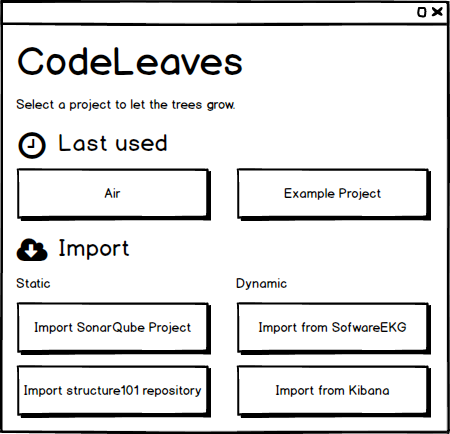
\includegraphics[width=.8\textwidth]{\figdir/project-selection-mockup}
  \caption{App-Menü}
  \label{fig:project-selection-mockup}
\end{figure}

Ist ein Projekt ausgewählt bzw. importiert, wird der Wald nach dem Layout, das in Kapitel \ref{ch:layout} erarbeitet wurde, generiert. Danach wird dem Nutzer die Möglichkeit geboten, den Wald so anzupassen, dass er genau die Informationen zeigt, die der Nutzer zu finden sucht.

Dies kann er ebenfalls mit dem App-Menu erreichen, das nun die wichtigsten Einstellungen des aktuellen Projekts zur Verfügung stellt. Im HoloLens Prototyp wurden nur essentielle Eistellungen eingebaut, die für die Nutzung des Prototyps unerlässlich sind. In Abbildung \ref{fig:project-selection-mockup} ist dagegen wiederum ein vollständiger Low-Fi Papier Prototyp zu sehen.

\begin{figure}[htb]
  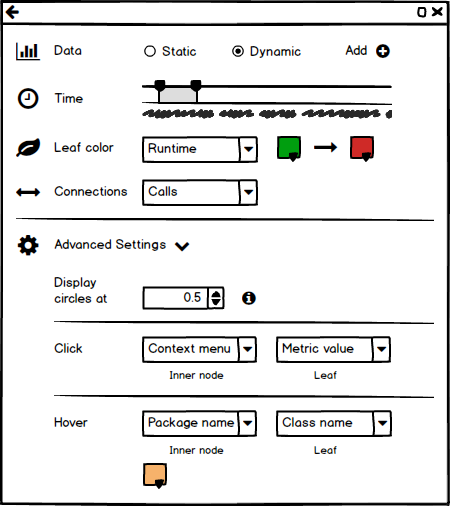
\includegraphics[width=.8\textwidth]{\figdir/app-menu-mockup}
  \caption{Mockup für die Einstellungen im App-Menü}
  \label{fig:project-selection-mockup}
\end{figure}

Mitunter wegen dem Akzeptanzkriterium \todo{Link auf Akzeptanz} ist es notwendig die aktuell dargestellten Metriken zu ändern. Die Zuordnung von Metriken für die Farbe der Blätter und die Stärke der Verbindungen nehmen deshalb als Drop-down zentrale Elemente im App-Menü ein.

Die zur Auswahl stehenden Metriken sind davon abhängig, ob der Nutzer gerade dynamische oder statische Daten betrachten möchte. Dynamische Daten beziehen sich immer auf einen bestimmten Zeitraum, wohingegen statische Informationen den Zustand eines Systems zu einem bestimmen Zeitpunkt widerspiegeln.

Deshalb wird als erstes die Wahl angeboten, ob statische oder dynamische Informationen betrachtet werden sollen. Mit dem "`Add"' neben dieser Auswahl kann der Nutzer Daten zu dem geladenen Projekt hinzufügen. Je nach dem welche Auswahl getroffen ist, kann der Nutzer darunter entweder einen Zeitpunkt -- in diesem Fall wird nur \textbf{ein} Schieberegler angezeigt -- oder einen Zeitraum angeben.

Die Drop-down-Listen für die dargestellten Informationen passen sich ebenfalls der Auswahl von "`Data"' an. Damit sind die wichtigsten Einstellungsmöglichkeiten abgedeckt und der Nutzer kann den Wald mit seiner Struktur und seinem Blätterdach erforschen.

Nach dem dem siebten von den sieben Interaction Design Prinzipien von Norman sollten die Interaktionsmöglichkeiten des Nutzers eigeschränkt werden, um ihn nicht zu überfordern \cite{norman2013design}.

\begin{figure}[htb]
  \centering
  \begin{subfigure}[b]{\fwidth}
    \centering
    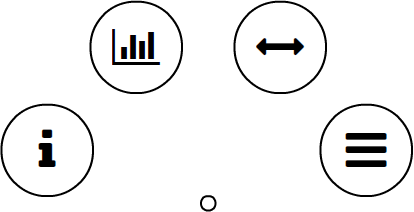
\includegraphics[scale=0.45]{figures/leaf-contextmenu}
    \subcaption{Initialer Zustand} \label{fig:leaf-contextmenu-initial}
  \end{subfigure}
  \hfill
  \begin{subfigure}[b]{\fwidth}
    \centering
  	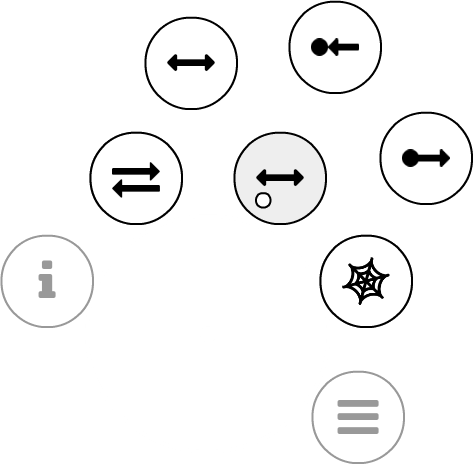
\includegraphics[scale=0.45]{figures/leaf-contextmenu-connections}
  	\subcaption{Unterauswahl im Kontextmenü} \label{fig:leaf-contextmenu-connections}
  \end{subfigure}
  \caption{Kontextmenü für ein Blatt} \label{fig:leaf-contextmenu}
\end{figure}

\section{Hover-Effekt}

\chapter{Zusammenfassung und Ausblick}
\label{ch:conclusion}

\section{Drilldown}
\section{Shared View für mehrere Nutzer}



% \appendix
% \chapter{Anhang}

\begin{figure}[htb]
  \includegraphics[width=.8\textwidth]{figures/sonarqube-import}
  \caption{Low-Fi Prototyp für den Import eines neuen Projekts anhand des Beispiels SonarQube}
  \label{fig:sonarqube-import}
\end{figure}

\begin{figure}[htb]
  \centering
  \begin{subfigure}[b]{\fwidth}
    \centering
    \includegraphics[scale=0.45]{figures/edge-contextmenu}
    \subcaption{Initialer Zustand} \label{fig:edge-contextmenu-initial}
  \end{subfigure}
  \hfill
  \begin{subfigure}[b]{\fwidth}
    \centering
    \includegraphics[scale=0.45]{figures/edge-contextmenu-connections}
    \subcaption{Unterauswahl für Verbindungen} \label{fig:edge-contextmenu-connections}
  \end{subfigure}
  \caption{Kontextmenü für einen inneren Knoten} \label{fig:edge-contextmenu}
\end{figure}

\begin{figure}[htb]
  \centering
  \begin{subfigure}[b]{\fwidth}
    \centering
    \includegraphics[scale=0.45]{figures/root-contextmenu}
    \subcaption{Initialer Zustand} \label{fig:root-contextmenu-initial}
  \end{subfigure}
  \hfill
  \begin{subfigure}[b]{\fwidth}
    \centering
    \includegraphics[scale=0.45]{figures/root-contextmenu-connections}
    \subcaption{Unterauswahl für Verbindungen} \label{fig:root-contextmenu-connections}
  \end{subfigure}
  \caption{Kontextmenü für eine Wurzel} \label{fig:root-contextmenu}
\end{figure}

\cleardoublepage
\printbibliography

\cleardoublepage
\footnotesize
\printindex

\end{document}
